\documentclass[ENG]{TFUOC}%IB: CASTELLÀ, CAT: CATALÀ, ENG: ANGLISH
\usepackage{pgfgantt}         % ← add these here
\usepackage{rotating}
\usepackage{float}
\usepackage{tikz}
\usepackage{natbib}   % ← add this line
\usepackage{array}
\usepackage{indentfirst}
\usepackage{eurosym}
\usepackage{enumitem} % glossary description list formatting


%Introduce Work Data
\title{Demand Forecasting for Inventory \newline Management Using Machine 
Learning}
\titcrt{} %Short title to appear in header
\author{Ona Mas I Serra}
\date{May, 2026}


\nomPDC{Lorena Polo Navarro}
\nomPRA{Susana Acedo Nadal}
\titulac{Master in Data Science}
\area{Forecasting in Industrial\newline and Business Environments}
\idioma{English}
\credits{12}
\parcla{Machine Learning, Demand Forecasting, Time Series Analysis, Predictive Modelling, Inventory Optimisation}

\licenc{ccByNcNd}
%Possible licenses
%ccByNcNd
%ccByNcSa
%ccByNc
%ccByNd
%ccBySa
%ccBy
%GNU
%copyright


%%%%%%%%%%
% Summary in language

\abstractidioma{

}

% Summary in English.
\abstractenglish{
Accurate demand forecasting is a critical challenge in industrial and business environments, where the ability to anticipate future demand directly impacts inventory efficiency, cost reduction, and supply chain performance. This Master's Final Project addresses two interconnected forecasting problems: demand forecasting for stock management and promotional demand forecasting, with data from a real company in the automotive sector.

The main objective of this work is to develop predictive models capable of estimating future demand for different products under both standard and promotional conditions. To this end, a data science methodology is applied, covering exploratory data analysis, data preprocessing and cleaning, feature engineering, and the application of machine learning, deep learning, and time series forecasting techniques. The promotional forecasting component specifically targets periods where demand behaviour is inherently more volatile and difficult to predict, requiring tailored modelling strategies.

The project also incorporates a bibliographic review of existing approaches in the field, allowing the refinement of objectives and the contextualisation of the proposed methodology within the current state of the art. Once the forecasting models are built and validated, an economic impact analysis is carried out, comparing the stock costs associated with the company's baseline forecasting approach against those obtained with the newly developed models.

The results aim to demonstrate the practical value of applying data science techniques to real industrial demand data, providing actionable insights for inventory optimisation and supply chain decision-making in the automotive industry.
}


\begin{document}

\estructura

\chapter*{Acknowledgements}

Aquesta tesi representa no només el resultat del meu esforç acadèmic, sinó també el suport que he rebut de moltes persones al llarg d'aquest viatge. És un plaer expressar la meva gratitud a tots aquells que han fet possible la realització d'aquesta obra.

En primer lloc, vull expressar el meu agraïment a la meva directora de tesi, la Lorena, per la seva orientació, paciència i motivació constants durant tot aquest procés. I a tot l'equip docent de la UOC pel seu suport i acompanyament durant aquests últims dos anys.

Un agraïment especial a l'equip d'Amazon, on he tingut l'oportunitat no només de créixer professionalment dins l'equip de Business Intelligence, sinó també per donar-me la motivació de continuar formant-me i aprofundint en el món de les dades.

Una menció especial al meu pare, que m'ha ensenyat que tot esforç té la seva recompensa i m'ha recolzat incondicionalment per arribar on estic ara. A la meva germana, una font d'inspiració per a mi, que em va donar la valentia d'acceptar aquest repte. A la resta de la família, que sempre han estat una font d'amor incondicional. I a la meva amiga Maria, que ha estat al meu costat en els moments difícils i ha celebrat amb mi cada petit èxit al llarg d'aquest camí.

Infine, un ringraziamento speciale a Tancredi. Grazie per avermi motivato e ispirato costantemente a essere la migliore versione di me stessa ogni giorno, e per il tuo supporto incondizionato, la tua pazienza e il tuo amore lungo tutto questo cammino. La tua presenza è stata, ed è, fondamentale. Ti amo.

\tableofcontents
\listoffigures
\listoftables


\chapter{Introduction}


\section{Context and justification of work}

Demand forecasting is the process of estimating the future quantity of goods or services that customers will require over a given time horizon. It is a critical component of supply chain management, as accurate forecasts directly influence inventory decisions, resource allocation, and operational costs.

Effective stock management depends fundamentally on the precision of demand forecasts. On one hand, holding excessive inventory ties up capital in unsold stock, increasing storage costs, insurance, and the risk of obsolescence. On the other hand, insufficient stock levels lead to stockouts, resulting in lost sales, production disruptions, and damage to customer relationships \citep{silver2016inventory, chopra2021supply}. Achieving the right balance between these two extremes requires forecasts that are as accurate as possible, so that inventory levels can be aligned as closely as possible with actual demand.

Demand is rarely stable: it is influenced by seasonality, promotions, and market trends, making accurate forecasting a significant challenge. Promotional periods are particularly difficult, as they introduce sudden demand spikes that conventional approaches struggle to capture reliably. In industrial environments such as the automotive sector, where supply chains are complex and the cost of stockouts can disrupt entire production lines, this challenge is especially critical.

Machine learning and data science techniques have opened new possibilities in this field, showing significant improvements over traditional statistical methods in complex, multi-product and promotional scenarios. This project addresses both standard and promotional demand forecasting using a real dataset from the automotive sector, aiming to develop predictive models that outperform the company's existing baseline approach and demonstrate a quantifiable impact on inventory costs.


\section{Personal Motivation}

My interest in this project arises from a combination of professional 
experience and a genuine curiosity to go deeper into the field of 
data science applied to forecasting. Working in an environment where 
demand forecasting directly impacts operational decisions has allowed 
me to appreciate both the importance and the complexity of accurately 
predicting future demand. However, this project goes beyond my current 
professional context: it represents an opportunity to build a solid 
methodological foundation, explore machine learning and time series 
techniques in a structured academic framework, and develop the skills 
needed to grow as a data scientist specialising in forecasting and 
supply chain optimisation.



\section{Work Objectives}

The main objective of this project is to develop a demand forecasting 
model capable of accurately estimating future demand for different 
products in an industrial context, covering both standard and 
promotional demand periods, and to evaluate its impact on inventory 
management and associated stock costs.

To achieve this, the following specific objectives are defined:

\begin{itemize}
    \item To conduct a bibliographic review of existing demand 
    forecasting approaches, identifying the most relevant machine 
    learning and time series techniques applied in industrial and 
    business environments.

    \item To explore, analyse, and prepare a real dataset from the 
    automotive sector, ensuring its quality and suitability for 
    predictive modelling.

    \item To design and implement a set of forecasting models for 
    standard demand, evaluating and comparing their performance using 
    appropriate accuracy metrics.

    \item To design and implement a forecasting model specifically 
    tailored to promotional demand periods, where demand behaviour 
    is inherently more volatile and harder to predict.

    \item To compare the performance of the developed models against 
    a baseline forecasting approach, assessing the improvement 
    achieved.

    \item To evaluate the economic impact of the developed models 
    on stock management, comparing inventory costs before and after 
    their application.
\end{itemize}

\section{Impact on sustainability, ethics-social and diversity}
\label{s:etic}

From a sustainability perspective, accurate demand forecasting 
contributes to more efficient inventory management, reducing 
overproduction, excess stock, and the waste associated with unsold 
goods. In the automotive sector, where supply chains are particularly 
resource-intensive, optimising stock levels can indirectly reduce 
unnecessary transportation and storage energy consumption, 
contributing to the goals of SDG 12 (Responsible Consumption and 
Production) and SDG 8 (Decent Work and Economic Growth) \citep{undp_sdg}. However, 
it is worth acknowledging that increased automation of forecasting 
processes could, in broader contexts, reduce the need for manual 
planning roles: a potential negative social impact that should be 
considered when deploying such solutions in real organisations.

Regarding ethics and data privacy, the dataset used in this project 
has been provided by the thesis tutor and corresponds to a real 
company in the automotive sector. It is fully anonymised, meaning 
no personal or commercially sensitive information is exposed, and 
therefore no privacy concerns are associated with this work.

Finally, this project does not involve human subjects, user 
profiling, or demographic data, so there are no direct concerns 
related to diversity or human rights. The work will be deposited 
in the UOC's open institutional repository (O2), making the 
findings freely accessible to any researcher or practitioner 
regardless of their background or institution.

\section{Methodology}

This project follows the CRISP-DM (Cross-Industry Standard 
Process for Data Mining) methodology \citep{wirth2000crisp}, which 
is the most widely adopted framework for data science and machine 
learning projects.

CRISP-DM defines six major phases, as illustrated in Figure 
\ref{fig:crisp-dm}:

\begin{figure}[H]
\centering
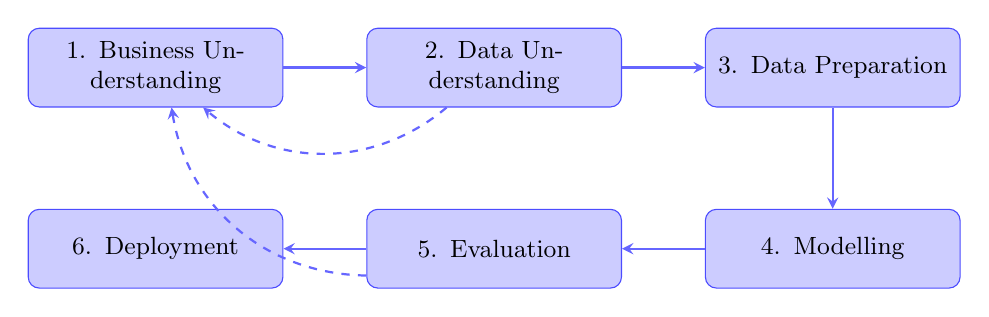
\begin{tikzpicture}[
    node distance=1.8cm,
    box/.style={rectangle, draw=blue!70, fill=blue!20, 
                text width=3cm, text centered, rounded corners, 
                minimum height=1cm, font=\small},
    arrow/.style={->, >=stealth, thick, blue!60}
]

\node (bu) [box] {1. Business Understanding};
\node (du) [box, right of=bu, xshift=2.5cm] {2. Data Understanding};
\node (dp) [box, right of=du, xshift=2.5cm] {3. Data Preparation};
\node (mo) [box, below of=dp, yshift=-0.5cm] {4. Modelling};
\node (ev) [box, left of=mo, xshift=-2.5cm] {5. Evaluation};
\node (de) [box, left of=ev, xshift=-2.5cm] {6. Deployment};

\draw [arrow] (bu) -- (du);
\draw [arrow] (du) -- (dp);
\draw [arrow] (dp) -- (mo);
\draw [arrow] (mo) -- (ev);
\draw [arrow] (ev) -- (de);

\draw [arrow, dashed, bend left=40] (du) to (bu);
\draw [arrow, dashed, bend left=40] (ev) to (bu);

\end{tikzpicture}
\caption{CRISP-DM methodology phases.}
\label{fig:crisp-dm}
\end{figure}

\begin{itemize}
    \item \textbf{Business Understanding:} This phase focuses on 
    understanding the project objectives and requirements from a 
    business perspective, then converting this knowledge into a 
    data science problem definition. In this project, this phase 
    involves defining the demand forecasting problem for inventory 
    management in the automotive sector, identifying the key 
    business questions to be addressed, and establishing the 
    expected impact of improved forecasting on stock costs and 
    supply chain efficiency.

    \item \textbf{Data Understanding:} This phase involves initial 
    data collection and exploration to become familiar with the 
    data, identify quality issues, and discover initial insights. 
    In this project, this corresponds to receiving the historical 
    demand dataset from the tutor, understanding its structure, 
    volume, and characteristics, and performing an initial 
    statistical analysis to identify patterns, seasonality, and 
    the behaviour of promotional versus standard demand periods.

    \item \textbf{Data Preparation:} This phase covers all 
    activities required to construct the final dataset from the 
    raw data, including cleaning, transformation, and feature 
    engineering. In this project, this involves handling missing 
    values and outliers, transforming variables into appropriate 
    formats, scaling numerical features, and creating new 
    predictive features such as calendar variables (day of week, 
    month, holidays), promotional indicators, and lag-based 
    features derived from historical demand patterns.

    \item \textbf{Modelling:} This phase involves selecting and 
    applying various modelling techniques, calibrating their 
    parameters, and training models on the prepared data. In this 
    project, multiple forecasting approaches will be implemented and compared, including classical time series methods (such as ARIMA), machine learning algorithms (such as XGBoost, LightGBM, and Random Forest), and deep learning methods (specifically LSTM networks), with particular 
    attention to models capable of capturing promotional demand 
    volatility.

    \item \textbf{Evaluation:} This phase assesses the models to 
    ensure they achieve the business objectives. In this project, 
    evaluation involves measuring forecast accuracy using 
    appropriate metrics (such as MAE, RMSE, or MAPE), comparing 
    model performance against baseline approaches, and analysing 
    model behaviour under standard and promotional demand 
    conditions separately.

    \item \textbf{Deployment:} In an industrial context, this 
    phase would involve integrating the model into production 
    systems. In this academic project, deployment corresponds to 
    the documentation of results and conclusions, and the 
    economic impact analysis comparing stock costs associated 
    with the baseline forecasting approach against those obtained 
    with the newly developed models.
\end{itemize}

The dashed arrows in Figure \ref{fig:crisp-dm} represent the iterative nature of the methodology, as insights gained in later phases may require revisiting earlier phases to refine the approach.


\section{Tools and Resources}

This project has been developed using the following tools and resources:

\begin{itemize}
    \item \textbf{Hardware:} MacBook Pro 14-inch (November 2024) 
    with Apple M4 chip and 16 GB of unified memory.

    \item \textbf{Programming language:} Python.


    \item \textbf{Documentation:} \LaTeX\, compiled and edited via Overleaf.
\end{itemize}




\section{Work schedule}

The project deliverables are structured across five modules:

\begin{itemize}
    \item \textbf{M1 -- Definition and Planning:} 
    Definition of the TFM scope, objectives, methodology, and 
    work schedule. Includes the ethics and confidentiality 
    declaration.

    \item \textbf{M2 -- State of the Art:} 
    Bibliographic review of existing demand forecasting approaches, 
    identifying the most relevant techniques and contextualising 
    the project within the current state of the art.

    \item \textbf{M3 -- Design and Implementation:} 
    Full development of the project, comprising data acquisition, 
    exploration, preparation, feature engineering, model 
    development, and evaluation.

    \item \textbf{M4 -- Documentation:} Writing of 
    the final thesis memory, including a preliminary submission, a final submission, and the audiovisual 
    presentation.

    \item \textbf{M5 -- Defence:} Submission of the 
    documentation to the tribunal and public defence of 
    the project.
\end{itemize}

The following Gantt chart provides a visual overview of the 
project timeline, as shown in Figure \ref{fig:gantt}.

\begin{figure}[H]
\centering
\begin{ganttchart}[
    hgrid,
    vgrid,
    x unit=0.5cm,
    y unit title=0.7cm,
    y unit chart=0.7cm,
    title/.style={fill=blue!30},
    title label font=\footnotesize,
    bar/.style={fill=blue!50},
    bar label font=\footnotesize,
    group/.style={fill=blue!70},
    group label font=\footnotesize\bfseries,
    milestone/.style={fill=darkblueUOC},
    milestone label font=\footnotesize,
    bar label node/.append style={align=left},
    group label node/.append style={align=left}
]{1}{18}

\gantttitle{TFM Schedule (Feb 19 -- Jun 26, 2026)}{18} \\
\gantttitle{Feb}{2}
\gantttitle{Mar}{4}
\gantttitle{Apr}{4}
\gantttitle{May}{4}
\gantttitle{Jun}{4} \\

\ganttgroup{M1: Definition \& Planning}{1}{2} \\
\ganttmilestone{M1 Submission (Mar 1)}{2} \\

\ganttgroup{M2: State of the Art}{3}{5} \\
\ganttmilestone{M2 Submission (Mar 22)}{5} \\

\ganttgroup{M3: Design \& Implementation}{6}{12} \\
\ganttbar{Data acquisition \& exploration}{6}{7} \\
\ganttbar{Data preparation \& cleaning}{7}{9} \\
\ganttbar{Feature engineering}{9}{10} \\
\ganttbar{Modelling \& evaluation}{10}{12} \\
\ganttmilestone{M3 Submission (May 10)}{12} \\

\ganttgroup{M4: Documentation}{13}{15} \\
\ganttbar{Preliminary memory (May 17)}{13}{13} \\
\ganttbar{Final memory (May 24)}{13}{14} \\
\ganttbar{Audiovisual presentation (Jun 2)}{14}{15} \\
\ganttmilestone{M4 Submission (Jun 2)}{15} \\

\ganttgroup{M5: Defence}{16}{18} \\
\ganttbar{Documentation to tribunal (Jun 5)}{16}{16} \\
\ganttbar{Preparation}{16}{18} \\
\ganttmilestone{Public defence (Jun 26)}{18} \\

\end{ganttchart}
\caption{TFM project schedule based on UOC academic calendar.}
\label{fig:gantt}
\end{figure}
\end{landscape}

\section{Project Deliverables}

This project produces the following deliverables:

\begin{itemize}

    \item \textbf{Thesis memory:} The present document, comprising 
    the academic report of the project, including the 
    bibliographic review, methodology, implementation, results, 
    and conclusions.

    \item \textbf{Source code:} A Python codebase covering the full data science 
    pipeline: data loading and exploration, preprocessing and 
    cleaning, feature engineering, model training and evaluation, 
    and economic impact analysis. The code is structured following 
    the CRISP-DM phases and is documented to ensure reproducibility.

    \item \textbf{Audiovisual presentation:} A recorded video 
    presentation summarising the project objectives, methodology, 
    results, and conclusions, submitted as part of the M4 
    deliverable.

    \item \textbf{Oral defence:} A public defence of the project 
    before the evaluation tribunal, scheduled for June 2026.

\end{itemize}

\section{Document Structure}

The remainder of this document is organised as follows:

\textbf{Chapter 2 -- State of the Art} presents a bibliographic 
review of the current landscape of demand forecasting research, 
covering classical statistical methods, machine learning and deep 
learning approaches, and the specific challenges of promotional 
demand forecasting. It also reviews the theoretical framework 
linking forecast accuracy to inventory costs, including the safety 
stock model and its relationship to forecast error, which 
underpins the economic impact analysis carried out in Chapter 3.

\textbf{Chapter 3 -- Design and Implementation} describes the 
full technical development of the project following the CRISP-DM 
methodology. It covers data acquisition and description, 
exploratory data analysis, data preprocessing and cleaning 
(including stock-out detection and demand reconstruction), feature 
engineering, model design and training, hyperparameter tuning, 
and evaluation of results across multiple forecasting algorithms. 
The chapter concludes with an economic impact analysis comparing 
inventory costs under the baseline forecasting approach and those 
achieved by the best-performing model.

\textbf{Chapter 4 -- Conclusions and Future Work} summarises the 
main findings of the project, reflects critically on the 
achievement of the initial objectives and the adequacy of the 
planned methodology, evaluates the ethical and sustainability 
impacts identified in Chapter 1, and outlines future lines of 
work that could not be explored within the scope of this project.



\chapter{State of the Art}

Demand forecasting has evolved significantly over the past decades, transitioning from purely statistical approaches to increasingly sophisticated machine learning methods capable of capturing complex, non-linear patterns in data. The automotive supplier industry provides a particularly compelling context for this evolution, as suppliers must simultaneously manage highly volatile demand across thousands of SKUs, structural shifts in component value pools, and persistent supply chain disruptions driven by geopolitical tensions and electrification uncertainty \citep{bcg2026automotive}. In this environment, accurate demand forecasting is not merely an operational convenience but a strategic necessity. This chapter reviews the current state of research in demand forecasting for inventory management, examining the techniques that have demonstrated effectiveness in industrial and business environments, with particular attention to the automotive sector. The review is structured around three interconnected themes: forecasting methodologies and their comparative performance, the specific challenge of promotional demand prediction, and the critical link between forecast accuracy and inventory cost optimisation.
\section{Forecasting Methodologies: From Statistical Models to Machine Learning}

The landscape of demand forecasting has undergone a fundamental transformation in recent years. Traditional statistical methods such as ARIMA (AutoRegressive Integrated Moving Average) and exponential smoothing have long served as the foundation of time series forecasting, offering interpretability and solid performance on data with clear trends and seasonal patterns \citep{makridakis2021m5}. These methods remain relevant, particularly for series with stable demand characteristics, where their simplicity and lower computational requirements represent practical advantages.

However, the M5 forecasting competition, one of the most comprehensive benchmarks in the field, demonstrated a clear shift toward machine learning approaches. The competition, which involved forecasting 42,840 hierarchical time series of Walmart retail sales, revealed that ``pure'' machine learning models consistently outperformed traditional statistical benchmarks \citep{makridakis2021m5findings}. Gradient boosting algorithms, particularly LightGBM and XGBoost, emerged as dominant techniques among the top-performing solutions, often used in combination with careful feature engineering that incorporated calendar variables, lag features, rolling statistics, and promotional indicators.

\citet{hyndman2021forecasting} provide a comprehensive treatment of traditional forecasting methods, demonstrating that exponential smoothing and ARIMA models each have distinct strengths depending on the characteristics of the time series. Exponential smoothing methods, particularly the ETS (Error, Trend, Seasonal) framework, tend to perform well on series with stable patterns and clear seasonality, while ARIMA models offer greater flexibility for capturing complex autocorrelation structures. Their analysis across diverse datasets underscores an important principle: the optimal forecasting method depends heavily on the characteristics of the underlying demand data, and no single approach dominates across all scenarios. This finding motivates the comparative approach adopted in the present work, where multiple methods are evaluated and the best-performing model is selected based on empirical performance.

In the automotive sector specifically, \citet{fu2026treebased} addressed the challenge of intermittent demand for electric vehicle spare parts using a two-stage random forest model. Their approach separately modelled demand occurrence probability and conditional demand size, recognising that automotive spare parts often exhibit sporadic demand patterns with many zero-demand periods. This methodology proved effective for managing the inherent sparsity in spare parts demand, providing a reliable and interpretable solution for inventory planning in manufacturing environments.

The emergence of deep learning architectures has added another dimension to the forecasting toolkit. Long Short-Term Memory (LSTM) networks, introduced by Hochreiter and Schmidhuber \citep{hochreiter1997lstm}, are a specialised type of recurrent neural network designed to capture long-range temporal dependencies in sequential data. Unlike tree-based methods, which rely on engineered lag features to incorporate temporal information, LSTM processes input data as ordered sequences, with its internal gating mechanism allowing it to selectively retain or discard information from previous time steps. This makes it particularly suited to demand forecasting scenarios where the temporal structure of the data carries predictive value, such as the build-up and post-promotional depression characteristic of promotional periods. \citet{barath2026lstm} demonstrated that LSTM networks can achieve competitive performance on industrial weekly time series when sufficient temporal structure is present, while \citet{mardotillah2025hybrid} showed that combining LSTM with classical statistical methods in a hybrid architecture can yield further accuracy improvements, with MAPE values of 3.97\%   compared to 12.39\%  for standalone ARIMA and 4.50\%  for standalone LSTM. In the present work, LSTM is included alongside tree-based methods to provide a comprehensive comparison across machine learning paradigms and to evaluate whether deep learning offers advantages for the specific demand patterns present in the automotive dataset.

The attention mechanism, originally developed for natural language processing, has also found application in time series forecasting. \citet{debnath2026hybrid} proposed an attention-based CNN-LSTM architecture that achieved strong performance on electricity demand forecasting, with an $R^2$ of 0.9677. While their application domain differs from retail demand, the underlying principles of capturing multi-scale features and assigning varying importance to different time steps are directly transferable to demand forecasting problems.

Recent research has also explored the application of foundation models and ensemble methods to demand forecasting. \citet{yang2025foundation} proposed a dual-strategy ensemble framework combining hierarchical partitioning by semantic levels (store, category, department) with architectural diversity across model backbones. Their experiments on the M5 benchmark demonstrated consistent improvements over strong baselines, suggesting that ensemble approaches remain highly effective even as individual model architectures become more sophisticated.

\section{The Challenge of Promotional Demand Forecasting}

Promotional periods represent one of the most challenging scenarios for demand forecasting, characterised by sudden demand spikes, price elasticity effects, and consumer behaviour that deviates significantly from normal patterns. Traditional forecasting methods, which rely heavily on historical regularities, often struggle to capture the volatile and event-driven nature of promotional demand. The challenge is further compounded by the fact that promotional effects vary substantially across products, price points, and customer segments, making it difficult to apply uniform modelling assumptions across a product portfolio. This variability motivates the use of machine learning approaches capable of learning product-specific promotional responses directly from data.

The M5 competition dataset explicitly included promotional variables (SNAP activities) and demonstrated the importance of incorporating such features into forecasting models. Top-performing solutions in the competition typically engineered extensive promotional features, including lag effects of past promotions, interaction terms between promotional status and other variables, and indicators for special events and holidays \citep{makridakis2021m5}. The ability to capture both the immediate demand uplift from promotions and the post-promotional demand depression, where consumers who stocked up during promotions subsequently reduce purchases, proved critical for accurate forecasting.

\citet{mitra2022hybrid} conducted a comparative study of demand forecasting models for a multi-channel retail company, proposing a hybrid RF-XGBoost-LR model that outperformed individual machine learning algorithms including random forest, XGBoost, gradient boosting, AdaBoost, and artificial neural networks. Their study incorporated promotional variables alongside store characteristics and regional factors, demonstrating the importance of a multi-dimensional approach to retail demand modelling.

The growing adoption of probabilistic forecasting represents another important trend in addressing promotional demand uncertainty. Rather than providing single point estimates, probabilistic approaches generate prediction intervals or full probability distributions, enabling decision-makers to quantify and manage uncertainty explicitly. The M5 competition included an ``Uncertainty'' challenge specifically focused on this capability, reflecting industry recognition that understanding forecast uncertainty is often as valuable as the point forecast itself \citep{makridakis2021m5}.

\section{Linking Forecast Accuracy to Inventory Costs}

While forecast accuracy metrics such as MAE, RMSE, and MAPE provide useful benchmarks for model comparison, the ultimate value of improved forecasting lies in its impact on business outcomes. In inventory management, this translates to reduced costs through optimised stock levels, fewer stockouts, and lower holding costs. Establishing this connection requires understanding both the components of inventory costs and the mathematical mechanisms through which forecast accuracy influences them.

\subsection{Components of Inventory Costs}

Inventory costs comprise several interrelated components that together determine the total cost of maintaining stock. Following the framework established by \citet{silver2016inventory} and \citet{chopra2021supply}, these costs can be categorised as follows:

\textbf{Holding costs} (or carrying costs) represent the total cost of maintaining inventory, including warehousing expenses, capital costs, insurance, and obsolescence risk. These costs are typically expressed as a percentage $h$ of the inventory value, with industry estimates ranging between 20 and 30 percent annually \citep{silver2016inventory}. For a product with unit cost $c$, the annual holding cost per unit is therefore $h \cdot c$.

\textbf{Stockout costs} (or shortage costs) capture the economic impact of inventory shortages. These include direct costs such as lost sales revenue and expedited shipping for emergency replenishment, as well as indirect costs such as customer dissatisfaction and potential long-term damage to customer relationships. Stockout costs are often more difficult to quantify than holding costs, but their magnitude can be substantial, particularly in industrial contexts where a missing component may halt an entire production line \citep{chopra2021supply}.

\textbf{Ordering costs} include the administrative expenses associated with placing and receiving orders, such as procurement processing, inspection, and receiving activities. While ordering costs are relevant for determining optimal order quantities (e.g., via the Economic Order Quantity model), they are less directly affected by forecast accuracy than holding and stockout costs.

\subsection{Safety Stock and the Forecast Error Relationship}
\label{s:safetystock}

Safety stock serves as the primary mechanism through which forecast accuracy influences inventory costs. Defined as the extra inventory maintained to buffer against demand uncertainty, safety stock levels are directly determined by forecast error characteristics. The standard formulation, as presented in \citet{silver2016inventory} and \citet{thomopoulos2015demand}, expresses safety stock as:

\begin{equation}
SS = z \cdot \sigma_e \cdot \sqrt{L}
\label{eq:safety_stock}
\end{equation}

\noindent where:
\begin{itemize}
    \item $SS$ is the safety stock quantity (units)
    \item $z$ is the safety factor corresponding to the desired service level (e.g., $z = 1.65$ for 95\% service level, $z = 2.33$ for 99\%)
    \item $\sigma_e$ is the standard deviation of forecast errors per period
    \item $L$ is the lead time in periods
\end{itemize}

This formulation reveals a critical insight: safety stock is directly proportional to forecast error variability. When forecast accuracy improves (i.e., $\sigma_e$ decreases), organisations can maintain the same service level with lower safety stock, or achieve higher service levels with the same inventory investment. \citet{tiacci2009approach} demonstrated empirically that the choice of forecasting method significantly impacts inventory system performance, with more accurate forecasting methods enabling substantial reductions in safety stock requirements while maintaining or improving service levels.

The associated holding cost for safety stock can then be expressed as:

\begin{equation}
C_{SS} = SS \cdot h \cdot c = z \cdot \sigma_e \cdot \sqrt{L} \cdot h \cdot c
\label{eq:ss_cost}
\end{equation}

\noindent where $h$ is the annual holding cost rate and $c$ is the unit cost of the product. This equation makes explicit the direct relationship between forecast error ($\sigma_e$) and inventory holding costs.

\subsection{Quantifying the Economic Impact of Forecast Improvement}

When comparing two forecasting approaches (a baseline method and an improved method) the potential cost savings from reduced safety stock can be calculated as:

\begin{equation}
\Delta C_{SS} = z \cdot \sqrt{L} \cdot h \cdot c \cdot (\sigma_{e,baseline} - \sigma_{e,improved})
\label{eq:cost_savings}
\end{equation}

For a portfolio of $n$ products, the total annual savings become:

\begin{equation}
\Delta C_{total} = \sum_{i=1}^{n} z_i \cdot \sqrt{L_i} \cdot h \cdot c_i \cdot (\sigma_{e,baseline,i} - \sigma_{e,improved,i})
\label{eq:total_savings}
\end{equation}

This formulation enables direct translation of forecast accuracy improvements (measured in terms of error standard deviation reduction) into monetary terms.

\subsection{The Newsvendor Model: Balancing Overage and Underage Costs}

A complementary perspective on the forecast-inventory relationship is provided by the newsvendor model, a classical framework for single-period inventory decisions under demand uncertainty \citep{raz2013newsvendor, silver2016inventory}. The model balances two types of costs:

\begin{itemize}
    \item \textbf{Overage cost} ($C_o$): the cost incurred per unit when inventory exceeds demand (holding cost, markdowns, obsolescence)
    \item \textbf{Underage cost} ($C_u$): the cost incurred per unit when demand exceeds inventory (lost profit margin, stockout penalties, customer goodwill loss)
\end{itemize}

The optimal order quantity $Q^*$ that minimises expected total cost is given by:

\begin{equation}
Q^* = F^{-1}\left(\frac{C_u}{C_u + C_o}\right)
\label{eq:newsvendor}
\end{equation}

\noindent where $F^{-1}$ is the inverse cumulative distribution function of demand. The ratio $\frac{C_u}{C_u + C_o}$ is known as the \textit{critical ratio} or \textit{critical fractile}.

When demand is assumed to follow a normal distribution with mean $\mu$ and standard deviation $\sigma$, the optimal order quantity can be decomposed as:

\begin{equation}
Q^* = \mu + z^* \cdot \sigma
\label{eq:newsvendor_normal}
\end{equation}

\noindent where $z^* = \Phi^{-1}\left(\frac{C_u}{C_u + C_o}\right)$ and $\Phi^{-1}$ is the inverse standard normal CDF. This decomposition separates the order quantity into \textit{cycle stock} ($\mu$, to cover expected demand) and \textit{safety stock} ($z^* \cdot \sigma$, to protect against uncertainty).

In practice, the standard deviation $\sigma$ in the newsvendor formulation represents the uncertainty in future demand, which is precisely what the forecast error captures. As \citet{ngartera2026stochastic} emphasised, there exists a ``persistent disconnect between forecasting models and the operational decisions they are intended to support.'' Their Decision Intelligence Framework addresses this gap by integrating probabilistic demand forecasting (via gradient boosting quantile regression) directly with newsvendor-based inventory optimisation, demonstrating that unified approaches yield superior business outcomes compared to treating forecasting and inventory decisions in isolation.

It is worth noting that while $\sigma$ in the newsvendor formulation 
represents the standard deviation of demand, the operational safety 
stock framework adopted in this work (Equation~\ref{eq:safety_stock}) 
uses $\sigma_e$, the standard deviation of forecast errors, which 
directly captures the improvement achievable through better forecasting 
models. In a multi-period replenishment context, $\sigma_e$ replaces 
$\sigma$ as the relevant measure of uncertainty, since it is the 
accuracy of the forecast (rather than the raw variability of demand) that determines the safety stock actually required.

\subsection{Total Cost Function for Model Comparison}

For retrospective evaluation of forecasting models, the total inventory-related cost over a historical period can be computed directly from forecast errors. Following the asymmetric cost structure implicit in the newsvendor model, the total cost for a given forecasting model over $T$ periods is:

\begin{equation}
TC = \sum_{t=1}^{T} \left[ C_o \cdot (F_t - D_t)^+ + C_u \cdot (D_t - F_t)^+ \right]
\label{eq:total_cost}
\end{equation}

\noindent where $F_t$ is the forecast for period $t$, $D_t$ is the actual demand, and $(x)^+ = \max(x, 0)$. This formulation recognises that overforecasting and underforecasting have different cost implications: overforecasting leads to excess inventory (incurring holding costs and potential obsolescence), while underforecasting leads to stockouts (incurring lost sales and customer service failures).

By computing equation \ref{eq:total_cost} for each candidate forecasting model using historical test data, one can directly compare models based on their economic impact rather than solely on statistical accuracy metrics. This approach aligns forecast evaluation with business objectives and provides a more meaningful basis for model selection in industrial applications.

\section{Evaluation Metrics and Methodological Considerations}

The selection of appropriate accuracy metrics is itself a significant 
methodological consideration in demand forecasting research. Common 
metrics include Mean Absolute Error (MAE), Root Mean Squared Error 
(RMSE), Mean Absolute Percentage Error (MAPE), and their variants 
\citep{vandeput2024forecast}. Each metric embodies different assumptions 
about error severity and scale sensitivity.

MAE provides an intuitive measure of average error magnitude in the 
same units as the original data, treating all errors equally regardless 
of direction or context:

\begin{equation}
    MAE = \frac{1}{T} \sum_{t=1}^{T} |D_t - F_t|
\end{equation}

RMSE, by squaring errors before averaging, gives greater weight to 
large deviations, making it appropriate when occasional large errors 
are particularly costly:

\begin{equation}
    RMSE = \sqrt{\frac{1}{T} \sum_{t=1}^{T} (D_t - F_t)^2}
\end{equation}

MAPE expresses errors as percentages of actual values, facilitating 
comparison across products with different demand scales, but can be 
problematic when actual values approach zero:

\begin{equation}
    MAPE = \frac{100\%}{T} \sum_{t=1}^{T} \left|\frac{D_t - F_t}{D_t}\right|
\end{equation}

For intermittent demand scenarios common in automotive spare parts, 
additional metrics may be required. The Mean Absolute Scaled Error 
(MASE) addresses some limitations of percentage-based metrics by 
scaling errors against a naive benchmark forecast, providing meaningful 
comparisons even for series with many zero values. The choice of metric 
should align with the business context and the relative costs of 
different error types.

Importantly, as highlighted in Section~\ref{s:safetystock}, the 
standard deviation of forecast errors ($\sigma_e$) plays a crucial 
role in determining safety stock requirements. While MAE and RMSE are 
commonly reported, it is the forecast error standard deviation that 
directly enters the safety stock calculation 
(Equation~\ref{eq:safety_stock}). Therefore, when the objective is to 
evaluate the inventory cost implications of different forecasting 
methods, tracking $\sigma_e$ alongside traditional accuracy metrics 
provides essential information for the economic impact analysis.

Cross-validation approaches for time series data require careful 
consideration of temporal dependencies. Standard k-fold 
cross-validation violates the sequential nature of time series, 
potentially leading to data leakage where future information influences 
predictions for past periods. Rolling forecast origin validation, where 
models are iteratively retrained on expanding windows and evaluated on 
subsequent periods, provides a more realistic assessment of 
out-of-sample performance \citep{makridakis2021m5findings}.


\section{Summary and Research Positioning}

The literature review reveals several key findings relevant to the present work. First, machine learning methods, particularly gradient boosting algorithms such as XGBoost and LightGBM, have demonstrated superior performance over traditional statistical methods for complex, multi-product forecasting scenarios, as evidenced by the M5 competition results. Second, the automotive sector presents specific challenges including intermittent demand patterns and supply chain volatility that require tailored modelling approaches. Third, promotional demand forecasting remains particularly challenging due to demand heterogeneity and event-driven patterns. Fourth, establishing the connection between forecast accuracy and inventory costs (through the safety stock relationship and the newsvendor framework) provides the economic justification for forecasting investments and enables quantification of business impact.

Table \ref{tab:literature_summary} summarises the key publications reviewed and their characteristics, positioning the present work within the current state of the art.

\setlength{\arrayrulewidth}{0.2pt}

\setlength{\arrayrulewidth}{0.2pt}

\begin{table}[H]
\centering
\small
\caption{Summary of reviewed literature and positioning of the present work.}
\label{tab:literature_summary}
\begin{tabular}{
    |>{\raggedright\arraybackslash}p{2.6cm}
    |>{\raggedright\arraybackslash}p{2.4cm}
    |>{\raggedright\arraybackslash}p{2.4cm}
    |>{\raggedright\arraybackslash}p{2.0cm}
    |>{\raggedright\arraybackslash}p{2.6cm}|}
\hline
\textbf{Reference} & \textbf{Sector} & \textbf{Algorithms} & \textbf{Metrics} & \textbf{Key Focus} \\
\hline
\citet{makridakis2021m5} & Retail & LightGBM, XGBoost, Ensemble & WRMSSE & M5 competition, hierarchical forecasting \\
\hline
\citet{fu2026treebased} & Automotive (EV) & Random Forest (two-stage) & MAE, RMSE & Intermittent spare parts demand \\
\hline
\citet{mitra2022hybrid} & Retail & RF, XGBoost, GB, ANN, Hybrid & MAE, RMSE, MAPE, $R^2$ & Multi-channel forecasting \\
\hline
\citet{mardotillah2025hybrid} & Energy & ARIMA-LSTM Hybrid & MAPE & Deep learning hybrid models \\
\hline
\citet{ngartera2026stochastic} & General & Gradient Boosting QR & Custom & Forecasting-inventory integration \\
\hline
\citet{tiacci2009approach} & General & Various & Service level, Cost & Forecast-inventory interaction \\
\hline
\citet{debnath2026hybrid} & Energy & CNN-LSTM (Attention) & $R^2$ & Multi-scale deep learning for demand forecasting \\
\hline
\citet{yang2025foundation} & Retail & Ensemble (Foundation Models) & WRMSSE & Dual-strategy ensembling on M5 benchmark \\
\hline

\textbf{Present work} & \textbf{Automotive} & \textbf{Naive Baseline, ARIMA, XGBoost, LightGBM, RF,LSTM} & \textbf{MAE, RMSE, MAPE, $\sigma_e$} & \textbf{Standard + promotional; economic impact} \\
\hline
\end{tabular}
\end{table}



The present work contributes to this body of research by applying machine learning forecasting techniques to real automotive sector data, addressing both standard and promotional demand scenarios, and explicitly quantifying the economic impact of forecast improvements on inventory costs using the theoretical framework presented in Section 3. This integrated approach (combining methodological rigour in forecasting with practical business impact assessment through safety stock cost analysis) addresses a gap identified in the literature between technical forecasting performance and operational value creation.

\chapter{Design and Implementation}

% chapter3.tex — Design and Implementation
% This file is included via % chapter3.tex — Design and Implementation
% This file is included via % chapter3.tex — Design and Implementation
% This file is included via \input{chapter3} in TFM_onamas.tex

This chapter presents the complete design and implementation of the demand forecasting system, following the CRISP-DM methodology introduced in Chapter~1. The work progresses from data acquisition and exploration through preprocessing, feature engineering, model development, evaluation, and finally the economic impact analysis that connects forecast accuracy to inventory cost savings.

\section{Data Origin}

\subsection{Data Acquisition}

The dataset used in this project was provided by the thesis supervisor and corresponds to real historical data from a company operating in the automotive sector. The data covers daily demand records for a portfolio of products, along with supplementary information on calendar events, promotional campaigns, and stock levels. All data was received in a single Microsoft Excel file (\texttt{Datos.xlsx}) containing four sheets, each representing a distinct dimension of the business context.

No personally identifiable information is present in the dataset, and all product references are anonymised using numerical identifiers, ensuring compliance with data privacy requirements as discussed in Section~\ref{s:etic}.

\subsection{Data Description}

The dataset comprises four tables, summarised in Table~\ref{tab:data_sheets}:

\begin{table}[H]
\centering
\small
\caption{Structure of the source dataset (\texttt{Datos.xlsx}).}
\label{tab:data_sheets}
\begin{tabular}{|l|l|r|p{5.5cm}|}
\hline
\textbf{Sheet} & \textbf{Key columns} & \textbf{Rows} & \textbf{Description} \\
\hline
Ventas (Sales) & producto, fecha, udsVenta & 654,588 & Daily unit sales per product \\
\hline
Calendario & fecha, bolOpen, bolHoliday & 732 & Calendar flags: business day and holiday indicators \\
\hline
Promociones & producto, fechaInicio, fechaFin & 1,894 & Promotional campaign periods per product \\
\hline
Stock & producto, fecha, udsStock & 654,588 & Daily stock levels per product \\
\hline
\end{tabular}
\end{table}

The sales sheet constitutes the core of the dataset, containing 654,588 daily observations across 894 unique products over a period of 732 days, spanning from November 2022 to November 2024. Each record represents the number of units sold for a specific product on a specific date.

The calendar sheet provides 732 daily records with two binary indicators: \texttt{bolOpen} (whether the business was open) and \texttt{bolHoliday} (whether the date was a public holiday). The promotions sheet contains 1,894 records defining promotional campaign windows through start and end dates for each product. The stock sheet mirrors the sales structure, recording the closing stock level for each product-date combination.

\subsection{Data Loading}

All four sheets were loaded into memory using the \texttt{pandas} library with the \texttt{openpyxl} engine. The sales and stock tables were merged on the shared keys \texttt{(producto, fecha)}, and the calendar information was joined on \texttt{fecha}. Promotional periods were transformed from date ranges into a binary indicator (\texttt{en\_promo}) at the product-date level, marking each observation as promotional or non-promotional based on whether the date fell within any active campaign for that product.

After merging, the resulting dataset contained 654,588 rows and served as the foundation for all subsequent analysis. The merged dataset was persisted in Apache Parquet format for efficient reloading in downstream scripts.


\section{Data Exploration}

\subsection{Data Summary}

An initial statistical summary of the target variable (\texttt{udsVenta}, units sold) revealed a highly skewed distribution. The mean daily sales per product were 1.42 units, with a median of zero and a standard deviation of 3.56. The maximum observed value was 99 units. This distribution reflects the nature of automotive parts demand, where the majority of product-day combinations register zero sales, punctuated by occasional larger orders.

Table~\ref{tab:sales_stats} presents the key descriptive statistics:

\begin{table}[H]
\centering
\small
\caption{Descriptive statistics of daily unit sales (\texttt{udsVenta}).}
\label{tab:sales_stats}
\begin{tabular}{|l|r|}
\hline
\textbf{Statistic} & \textbf{Value} \\
\hline
Count & 654,588 \\
Mean & 1.42 \\
Std. deviation & 3.56 \\
Median (50\%) & 0.00 \\
75th percentile & 1.00 \\
95th percentile & 7.00 \\
Maximum & 99 \\
Zero-sales proportion & 64.5\% \\
\hline
\end{tabular}
\end{table}

The high proportion of zero-sales observations (64.5\%) is a defining characteristic of this dataset and has important implications for model selection and evaluation, as discussed in subsequent sections.

\begin{figure}[H]
\centering
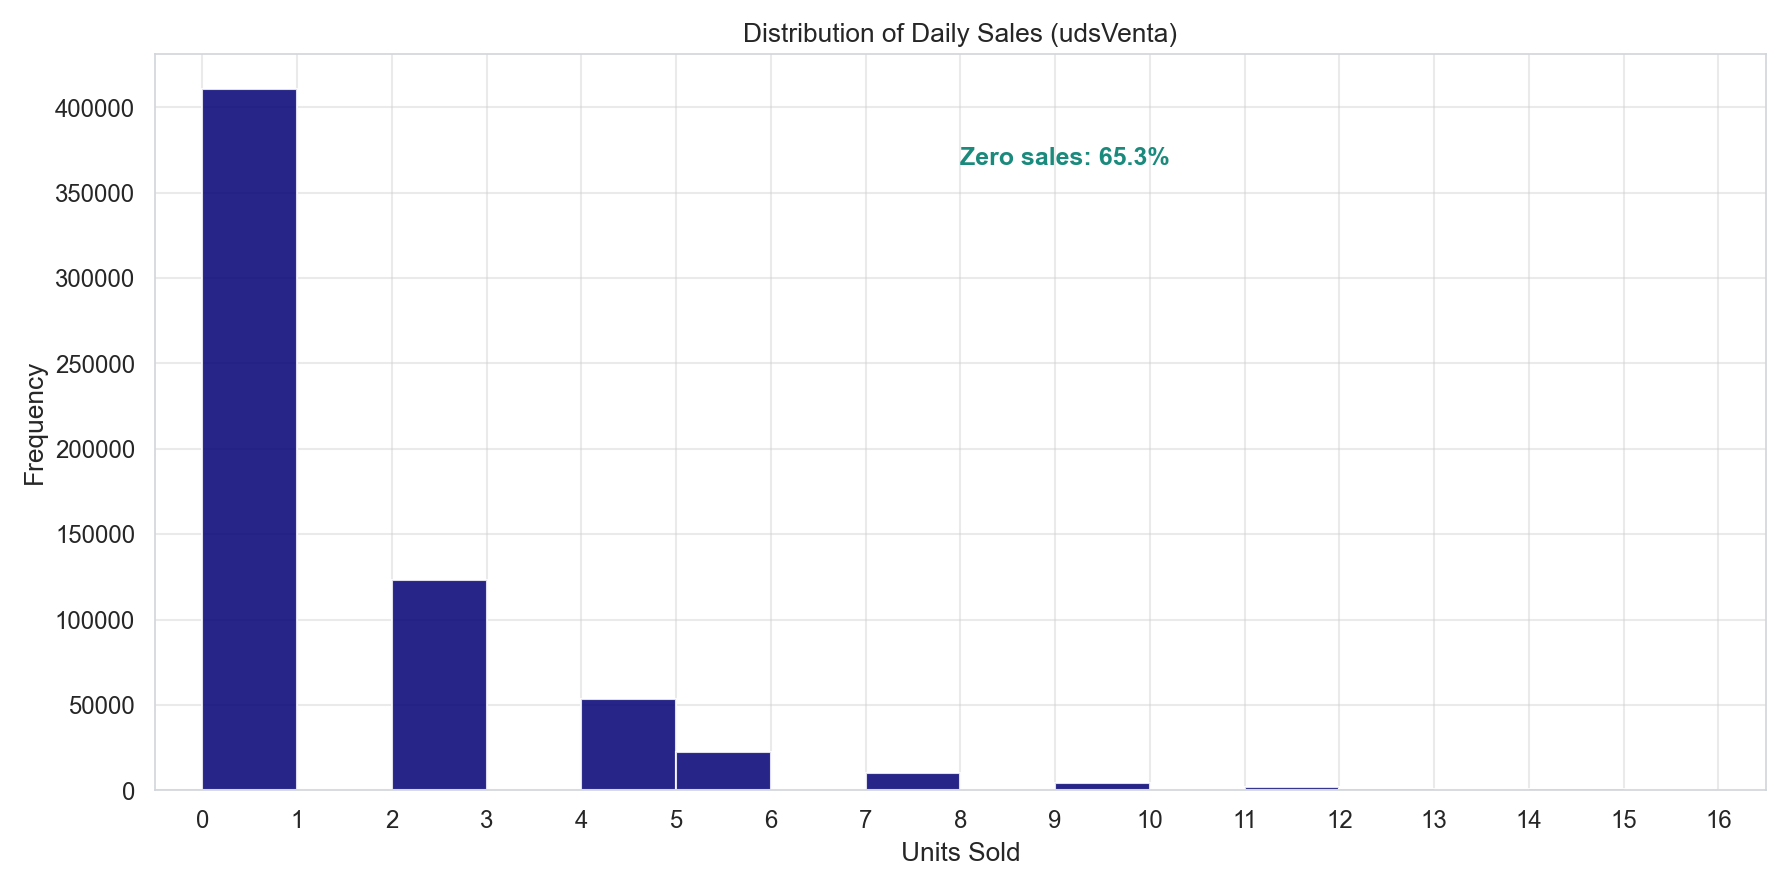
\includegraphics[width=0.85\textwidth]{figures/01_sales_distribution.png}
\caption{Distribution of daily unit sales (\texttt{udsVenta}). The histogram confirms the extreme right skew, with the majority of observations at zero.}
\label{fig:sales_distribution}
\end{figure}

\subsection{Statistical Analysis}

The exploratory analysis examined demand patterns across several dimensions:

\textbf{Day-of-week patterns.} Sales exhibit a clear weekly cycle, with the highest volumes on weekdays (Monday through Friday) and a sharp decline on Saturdays. Sunday sales are near zero, consistent with the business being closed on Sundays as indicated by the \texttt{bolOpen} calendar flag. This weekly seasonality motivates the inclusion of day-of-week features and the use of a lag-7 naive baseline (same weekday, previous week) as the primary benchmark.

\begin{figure}[H]
\centering
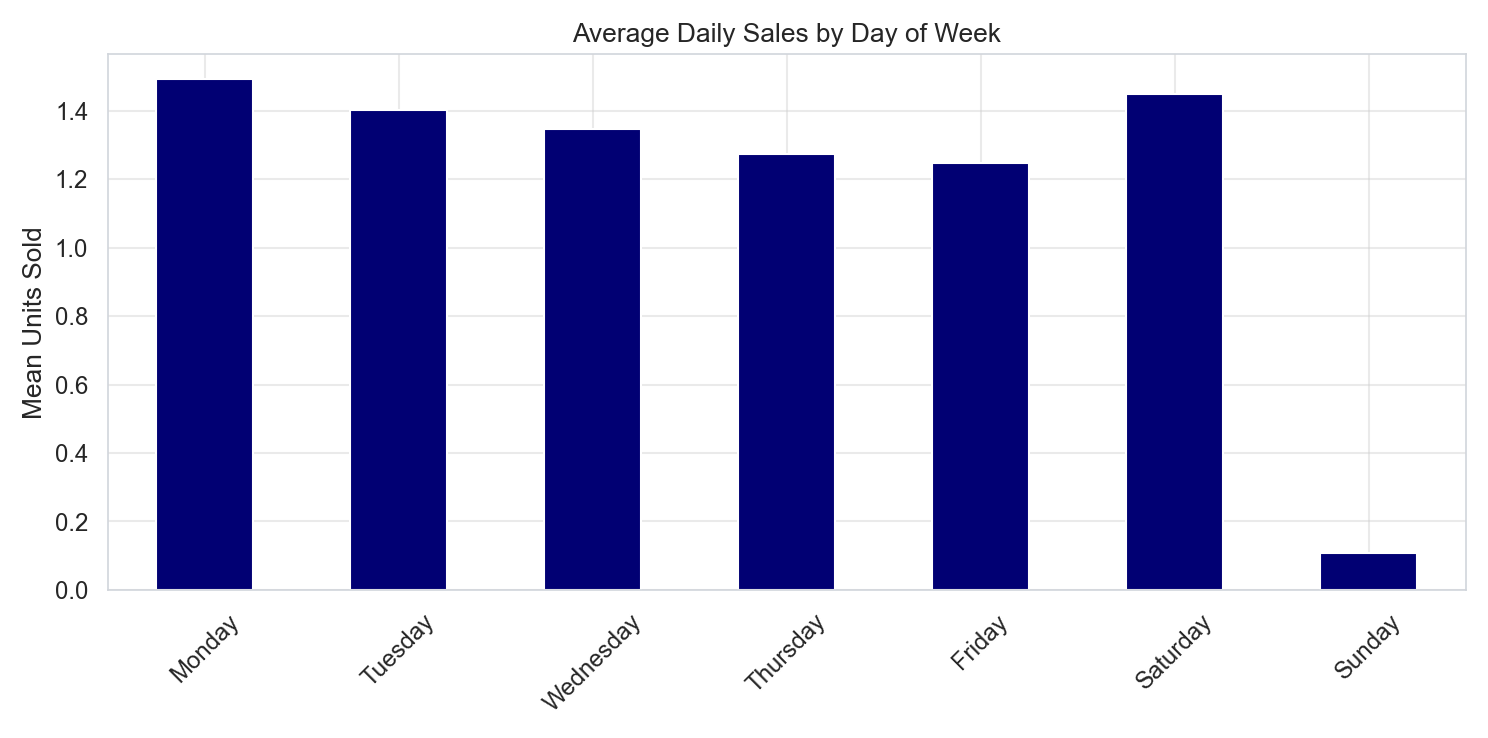
\includegraphics[width=0.85\textwidth]{figures/02_sales_by_day_of_week.png}
\caption{Average daily sales by day of the week. The weekly cycle is clearly visible, with near-zero sales on Sundays.}
\label{fig:sales_by_dow}
\end{figure}

\textbf{Monthly and seasonal patterns.} Monthly aggregated sales show moderate variation across the year, without a single dominant seasonal peak. However, certain months consistently show higher activity, suggesting that calendar-based features (month, week of year) may contribute predictive value.

\textbf{Promotional effects.} Comparing sales during promotional and non-promotional periods revealed that mean sales during promotions (1.83 units) were slightly higher than during non-promotional periods (1.38 units). However, the difference is modest, and the promotional flag alone does not capture the full complexity of promotional demand dynamics, which motivated the engineering of additional promotional features described in Section~3.4.

\begin{figure}[H]
\centering
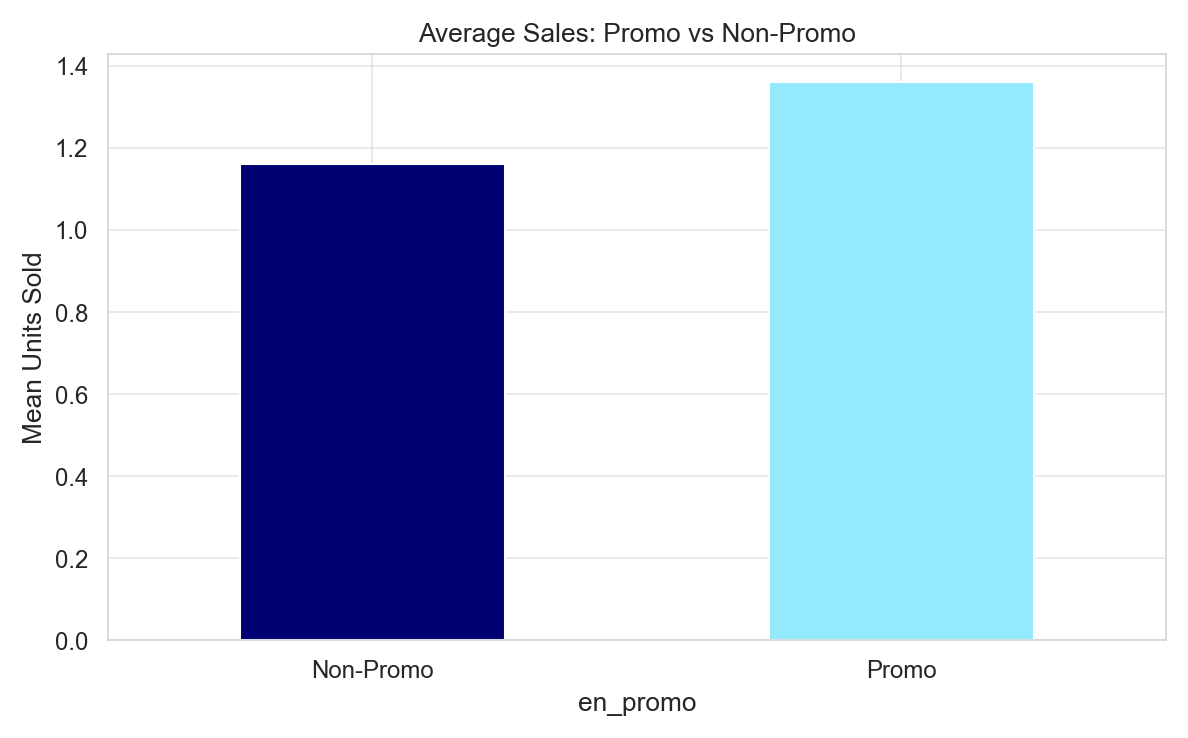
\includegraphics[width=0.85\textwidth]{figures/05_promo_vs_nonpromo.png}
\caption{Comparison of sales distributions during promotional and non-promotional periods.}
\label{fig:promo_vs_nonpromo}
\end{figure}

\textbf{Autocorrelation structure.} Autocorrelation analysis on a sample of products confirmed significant positive autocorrelation at lags 1, 7, 14, and 28, with the strongest signal at lag 7 (weekly periodicity). This finding directly supports the creation of lag features at these intervals and validates the choice of lag-7 as the naive baseline.

\begin{figure}[H]
\centering
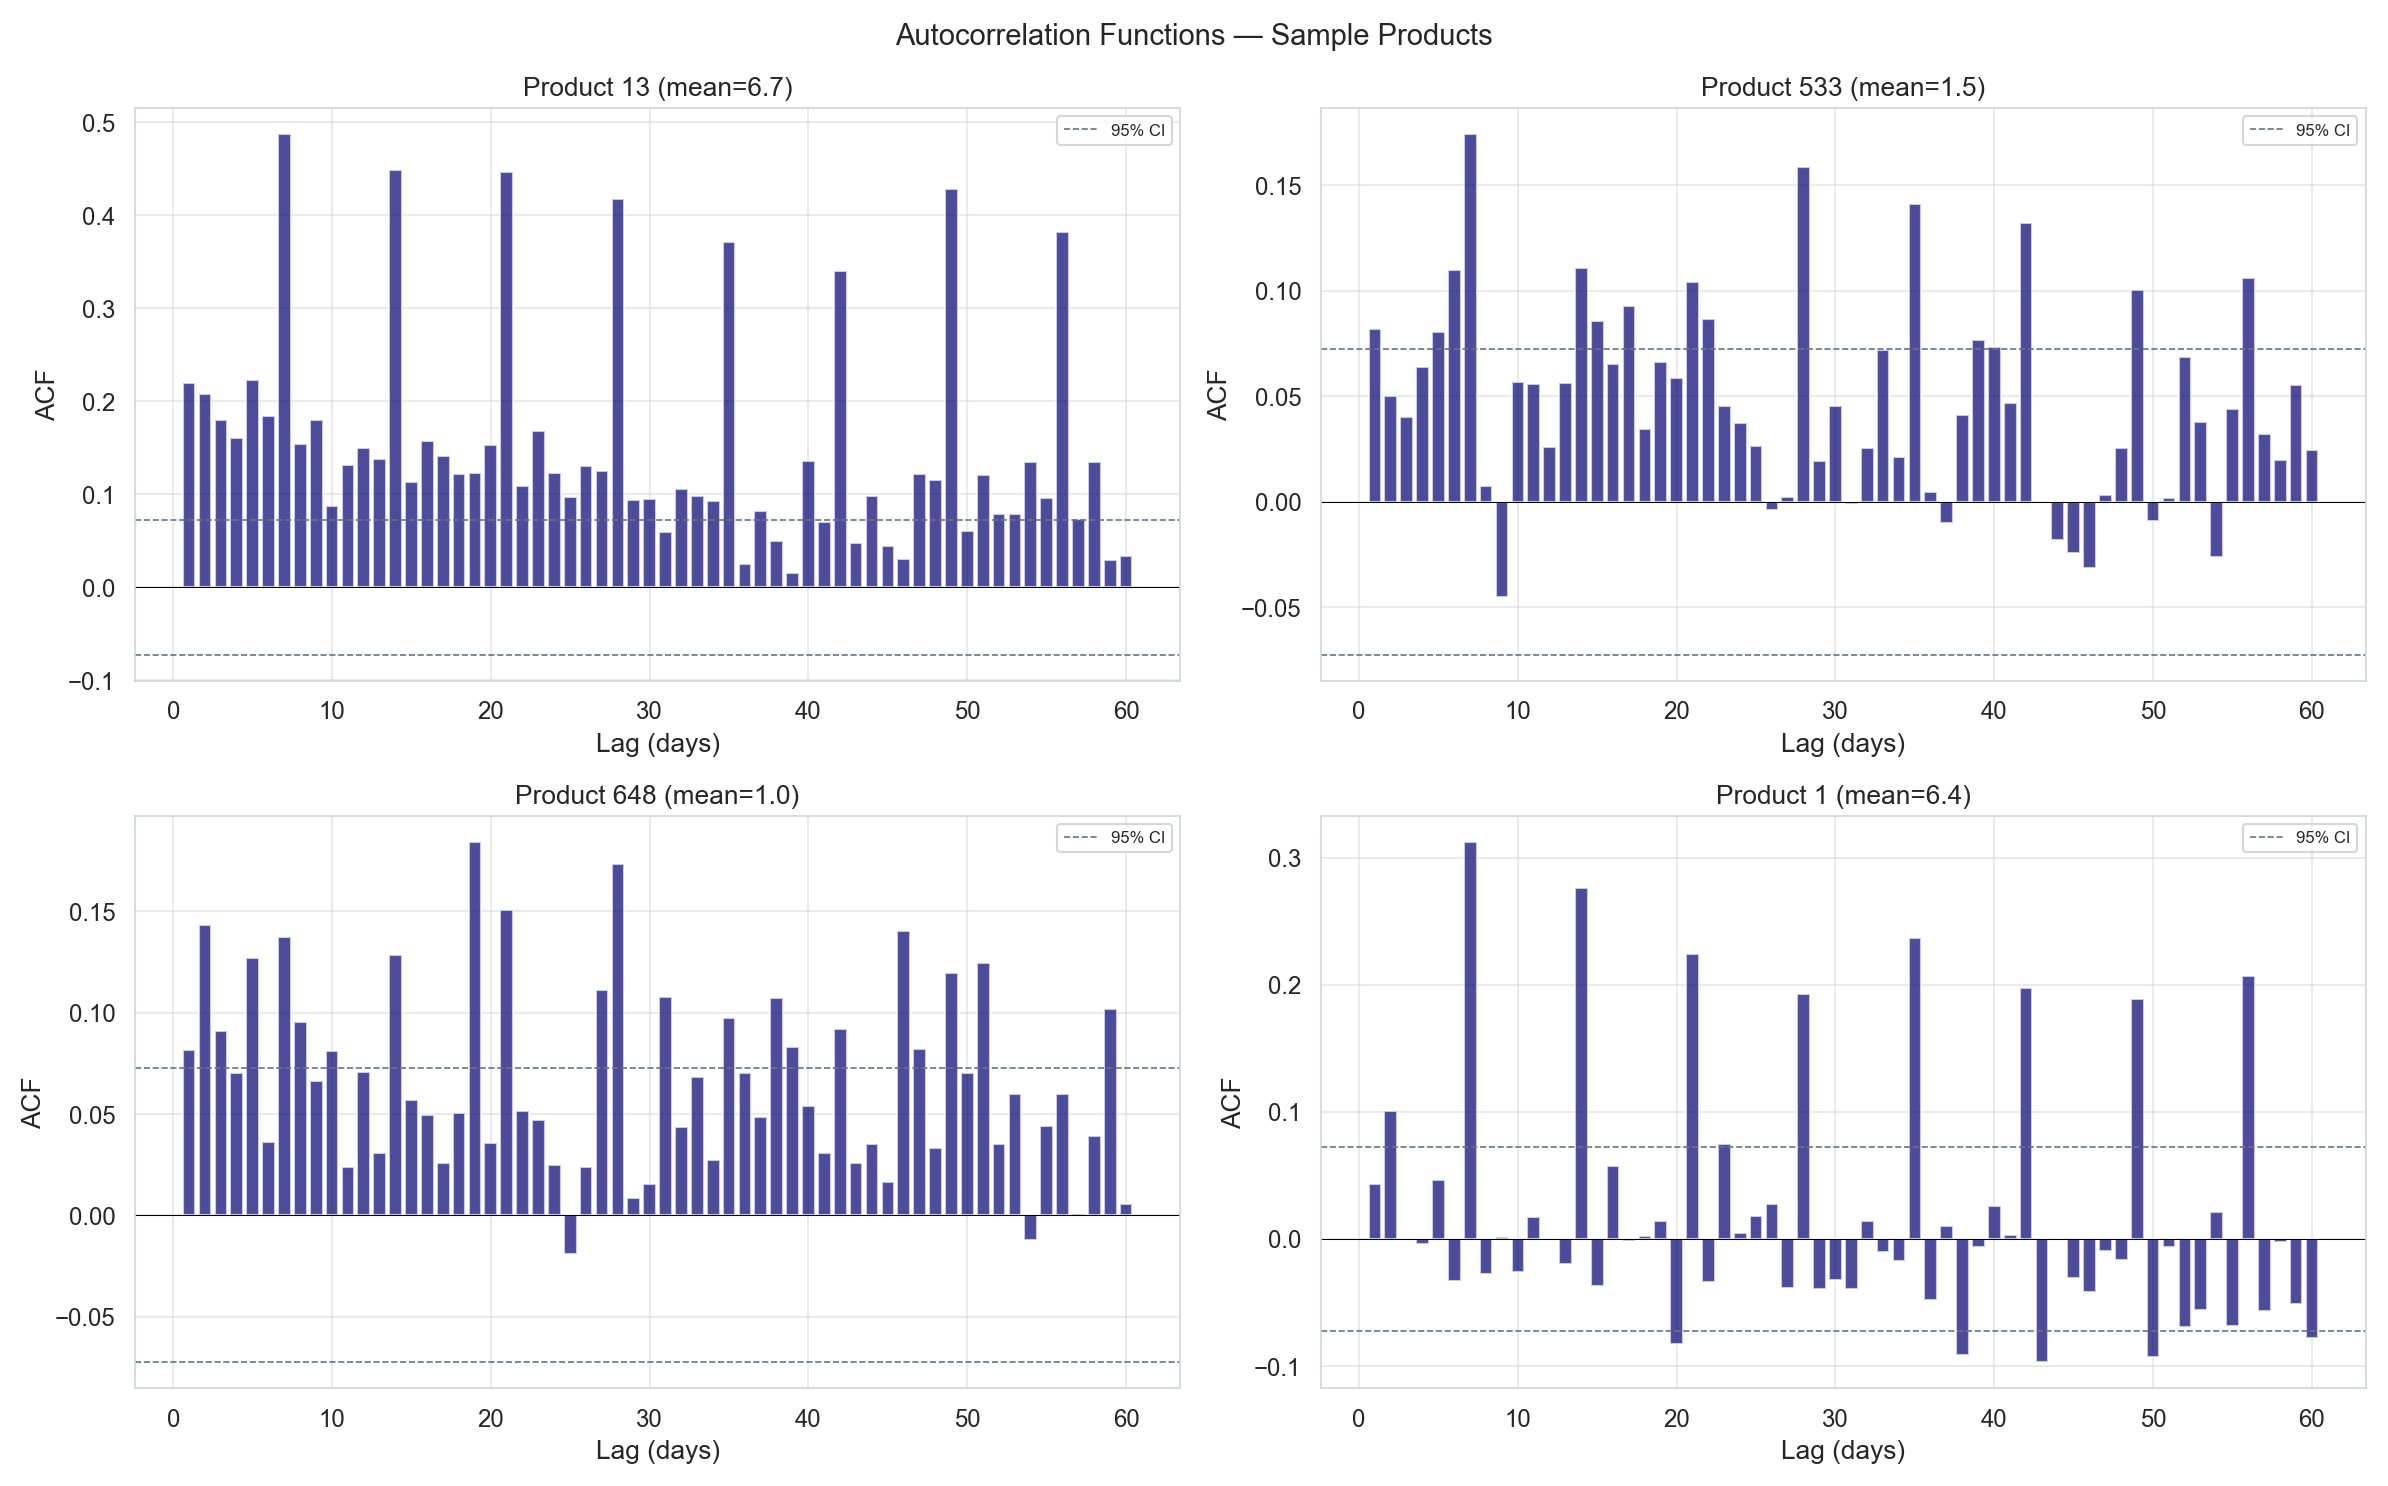
\includegraphics[width=0.85\textwidth]{figures/08_autocorrelation_sample.png}
\caption{Autocorrelation function (ACF) for a sample of products, showing significant positive autocorrelation at weekly intervals.}
\label{fig:autocorrelation}
\end{figure}

\subsection{Data Quality Analysis}

The data quality assessment identified the following issues:

\textbf{Missing values.} No explicit missing values were found in any of the four source tables. However, implicit gaps exist where lag features cannot be computed for the earliest dates in each product's history (addressed during feature engineering).

\textbf{Negative values.} No negative sales or stock values were present in this dataset.

\textbf{Stock breaks.} A stock break is defined as a day where both sales and stock are zero, potentially indicating that demand existed but could not be fulfilled due to inventory unavailability. Approximately 3.9\% of observations met this criterion. These were treated during data cleaning by imputing the product's historical mean sales for the corresponding weekday.

\textbf{Outliers.} Outlier detection was performed using a threshold of 1.75 times the interquartile range (IQR) per product. This identified approximately 11,400 observations (1.75\% of the dataset) as outliers, which were capped at the upper threshold value. The IQR-based approach was preferred over a fixed standard deviation threshold to account for the varying demand scales across products.


\section{Data Preparation}

\subsection{Data Cleaning}

The data cleaning process addressed the two quality issues identified during exploration:

\begin{enumerate}
    \item \textbf{Stock break imputation:} For observations where both \texttt{udsVenta} and \texttt{udsStock} were zero, the sales value was replaced with the mean sales for that product on the same weekday, computed over the preceding 30 days. This approach assumes that zero sales on a day with zero stock reflects a supply-side constraint rather than genuine zero demand, and uses a localised historical average to provide a reasonable demand estimate.

    \item \textbf{Outlier capping:} Values exceeding 1.75 $\times$ IQR above the 75th percentile for each product were capped at the threshold value. This preserves the general distribution shape while limiting the influence of extreme observations on model training. A total of 11,400 values (1.75\% of the dataset) were capped.
\end{enumerate}

After cleaning, the dataset retained its original 654,588 rows with no records removed, ensuring that the temporal continuity required for lag feature computation was preserved.

\subsection{Data Transformation}

The date column (\texttt{fecha}) was parsed into a \texttt{datetime} type, and the dataset was sorted by product and date to ensure correct temporal ordering for all subsequent operations. The promotional periods from the source data were transformed from date-range format into a daily binary indicator (\texttt{en\_promo}), assigned at the product-date level.

No logarithmic or power transformations were applied to the target variable. While such transformations can stabilise variance in skewed distributions, the tree-based models used in this work (Random Forest, XGBoost, LightGBM) are inherently robust to non-normal distributions and do not require target transformation for effective learning.

\subsection{Data Scaling}

Feature scaling (standardisation or normalisation) was not applied for the tree-based models, as decision tree ensembles are invariant to monotonic transformations of input features. The split-based learning mechanism of these algorithms operates on feature rankings rather than absolute values, making scaling unnecessary.

For the LSTM model, min-max normalisation was applied to all input features to facilitate gradient-based optimisation. Each feature was scaled to the $[0, 1]$ range using the training set statistics, and the same transformation was applied to the validation and test sets to prevent information leakage. Predictions were inverse-transformed back to the original scale before computing evaluation metrics.

\section{Feature Engineering}

Feature engineering is a central component of this work. A comprehensive set of 36 engineered features was designed to capture temporal dependencies, demand dynamics, and promotional effects. The features are organised into five categories, summarised in Table~\ref{tab:features}.

\begin{table}[H]
\centering
\small
\caption{Engineered features by category.}
\label{tab:features}
\begin{tabular}{|l|p{7cm}|r|}
\hline
\textbf{Category} & \textbf{Features} & \textbf{Count} \\
\hline
Original variables & udsStock, bolOpen, bolHoliday, en\_promo & 4 \\
\hline
Calendar features & year, month, day\_of\_week, week\_of\_year, week\_of\_month, is\_weekend, is\_month\_start, is\_month\_end & 8 \\
\hline
Lag features & lag\_1, lag\_7, lag\_14, lag\_28 & 4 \\
\hline
Rolling statistics & roll\_mean/std/min/max at 7, 14, and 28-day windows; ewma\_7, ewma\_28 & 14 \\
\hline
Promotional features & days\_since\_promo\_end, post\_promo\_7d, promo\_x\_lag7 & 3 \\
\hline
Product-level statistics & prod\_mean\_sales, prod\_std\_sales, prod\_median\_sales & 3 \\
\hline
\multicolumn{2}{|r|}{\textbf{Total}} & \textbf{36} \\
\hline
\end{tabular}
\end{table}

\textbf{Lag features} capture the autoregressive structure identified during exploration. The lag-7 feature (same weekday, previous week) serves dual purpose: it is used directly as the naive baseline forecast and as an input feature for the machine learning models. Lags at 1, 14, and 28 days capture short-term momentum, biweekly patterns, and monthly cycles respectively.

\textbf{Rolling statistics} provide smoothed representations of recent demand behaviour. For each window size (7, 14, and 28 days), the mean, standard deviation, minimum, and maximum of past sales are computed. Additionally, exponentially weighted moving averages (EWMA) with spans of 7 and 28 days provide adaptive smoothing that gives greater weight to more recent observations.

\textbf{Promotional features} go beyond the binary indicator to capture the temporal dynamics of promotions. The \texttt{days\_since\_promo\_end} feature tracks the recency of the last promotional period, \texttt{post\_promo\_7d} flags the week immediately following a promotion (to capture post-promotional demand depression), and \texttt{promo\_x\_lag7} is an interaction term between the promotional flag and the lag-7 sales value.

All lag and rolling features were computed strictly using past data to prevent information leakage. Observations where lag features could not be computed (the first 28 days of each product's history) were dropped, reducing the dataset from 654,588 to 629,370 rows. The final feature matrix was saved in Parquet format for use in the modelling phase.

\begin{figure}[H]
\centering
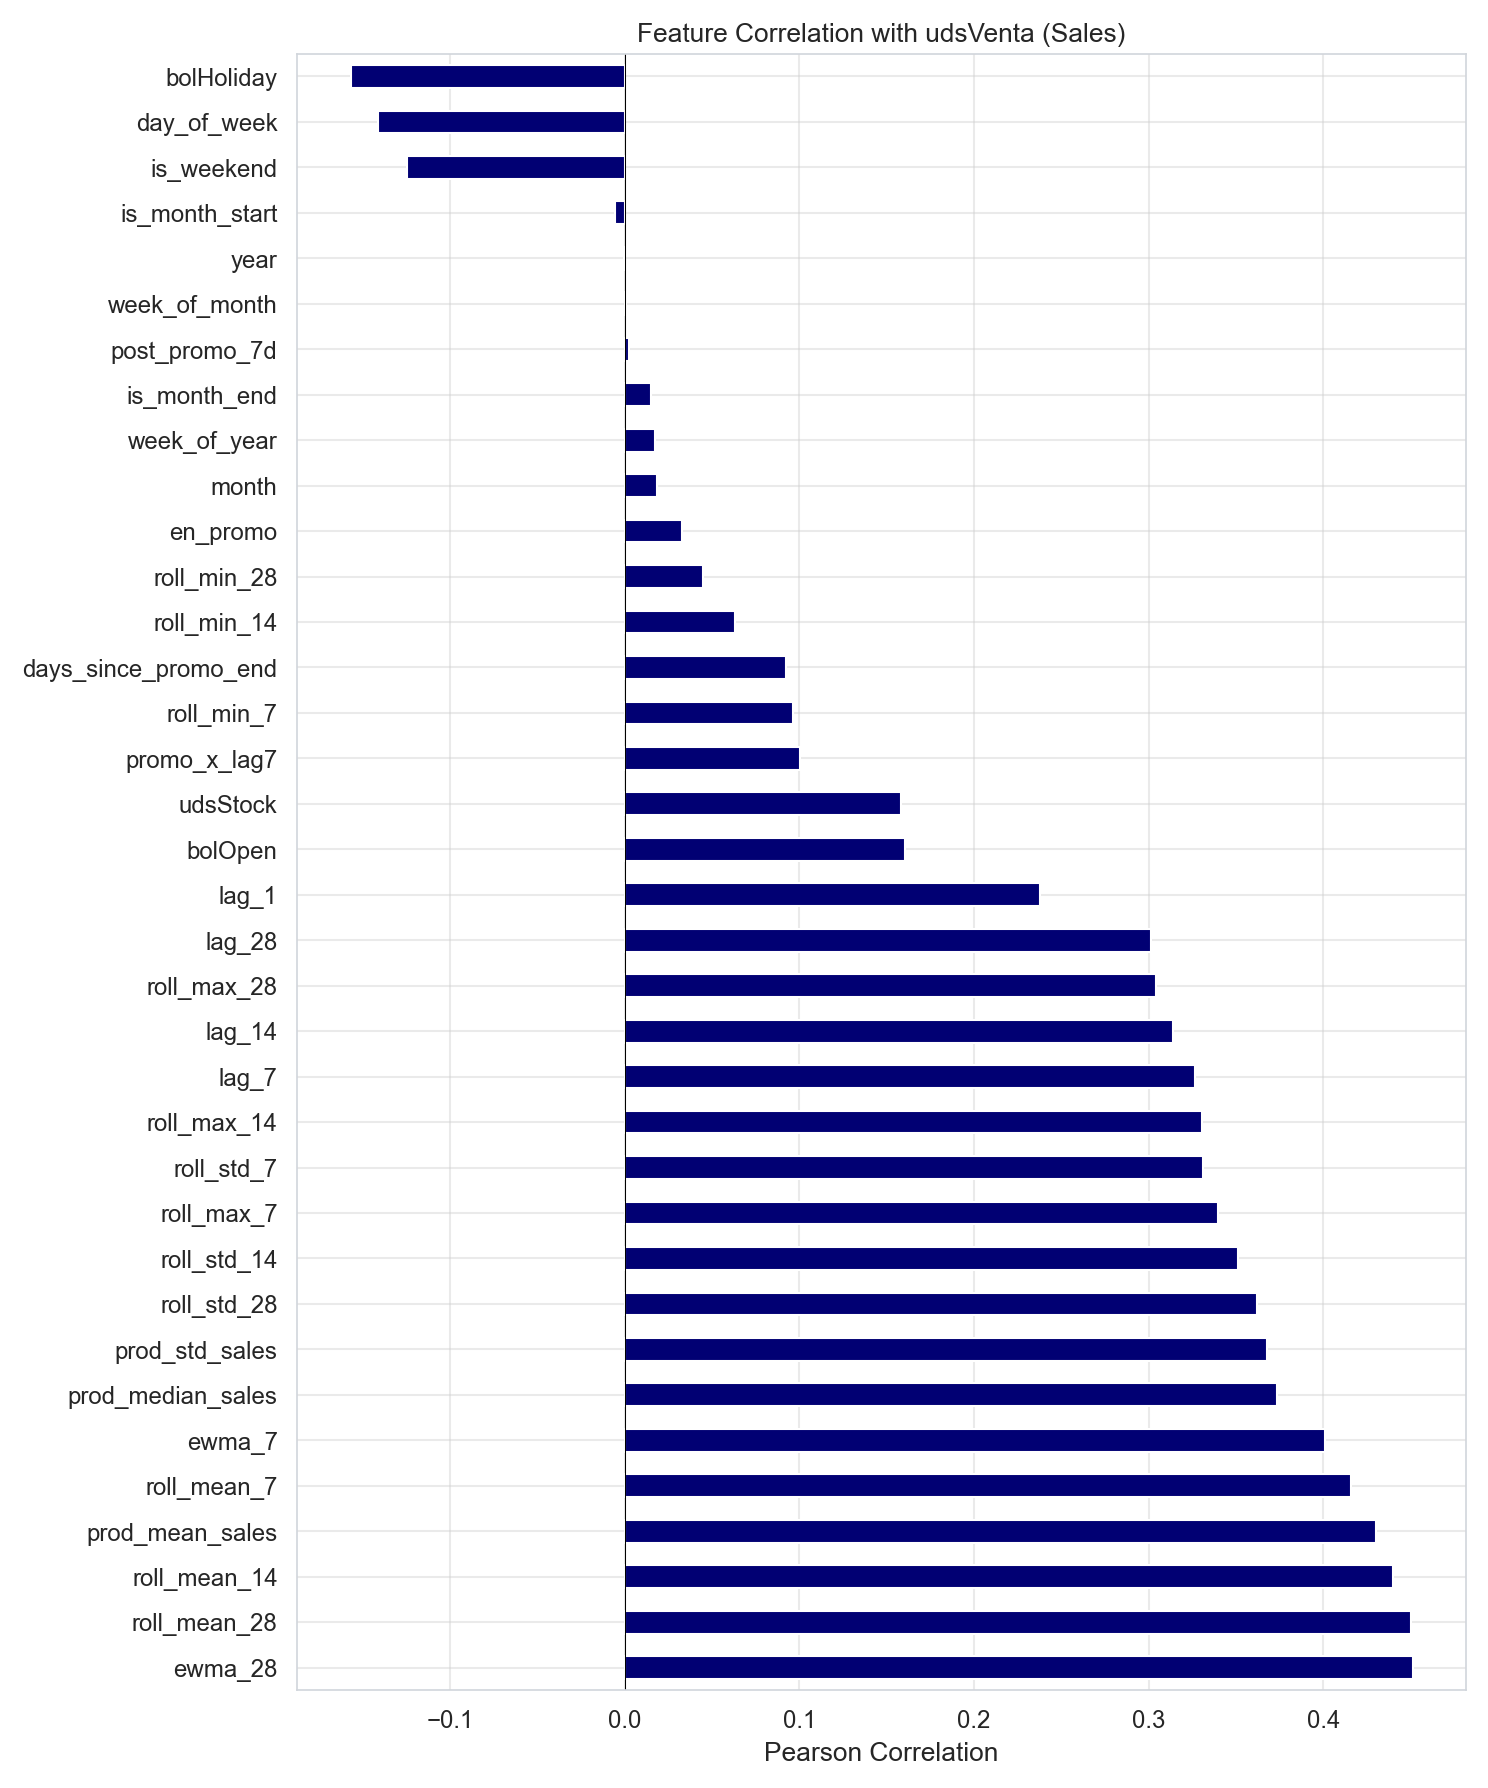
\includegraphics[width=0.95\textwidth]{figures/10_feature_correlations.png}
\caption{Correlation matrix of the engineered features. Strong correlations are visible among rolling statistics at different window sizes, confirming the presence of redundant but complementary temporal signals.}
\label{fig:feature_correlations}
\end{figure}


\section{Modelling}

\subsection{Model Selection}

Four forecasting approaches were implemented, spanning a naive baseline and three gradient boosting / ensemble methods:

\begin{enumerate}
    \item \textbf{Naive baseline (lag-7):} The simplest possible forecast, predicting that demand on any given day equals the demand observed on the same weekday of the previous week. This baseline exploits the strong weekly autocorrelation identified during exploration and provides a meaningful benchmark against which machine learning models must demonstrate improvement.

    \item \textbf{ARIMA (Seasonal):} A classical time series approach fitted per product using the \texttt{auto\_arima} implementation from the \texttt{pmdarima} library. Each product's demand series was modelled with seasonal ARIMA (SARIMA) with weekly periodicity ($m=7$), automatically selecting the optimal $(p,d,q)(P,D,Q)_7$ orders via stepwise search. ARIMA serves as the classical statistical baseline, representing the best that traditional time series methods can achieve without engineered features.

    \item \textbf{Random Forest:} An ensemble of decision trees trained on bootstrap samples with random feature subsets \citep{hyndman2021forecasting}. Random Forest provides robust predictions with built-in protection against overfitting through bagging and feature randomisation.

    \item \textbf{XGBoost:} A gradient boosting framework that builds trees sequentially, with each tree correcting the errors of its predecessors. XGBoost incorporates L1 and L2 regularisation, column subsampling, and efficient handling of sparse data, making it well-suited to the high proportion of zero-demand observations in this dataset.

    \item \textbf{LightGBM:} A gradient boosting implementation that uses histogram-based splitting and leaf-wise tree growth, offering faster training times than XGBoost while maintaining competitive accuracy. LightGBM was among the dominant algorithms in the M5 forecasting competition \citep{makridakis2021m5findings}.

    \item \textbf{LSTM (Long Short-Term Memory):} A recurrent neural network architecture designed to capture long-range temporal dependencies in sequential data \citep{hochreiter1997lstm}. Unlike tree-based methods, which rely on engineered lag features, LSTM processes input data as ordered sequences, with its internal gating mechanism allowing it to selectively retain or discard information from previous time steps. The model was implemented in PyTorch with a single LSTM layer (32 hidden units), trained on standardised features using 14-day input sequences.
\end{enumerate}

All tree-based models were trained on the full set of 33 input features (the 36 engineered features minus the 3 product-level statistics used only for reference). ARIMA was fitted per product on the raw sales series without engineered features, as is standard for classical time series methods. The LSTM model received the same 33 features as the tree models, but processed them as ordered sequences rather than independent observations. All predictions were clipped to a minimum of zero to prevent negative forecast values.

\subsection{Definition of Accuracy Indicators}

Four complementary metrics were used to evaluate forecast performance, as introduced in Chapter~2:

\begin{itemize}
    \item \textbf{MAE} (Mean Absolute Error): average absolute deviation between forecast and actual demand, in the same units as the target variable.
    \item \textbf{RMSE} (Root Mean Squared Error): penalises larger errors more heavily than MAE, providing a measure sensitive to occasional large deviations.
    \item \textbf{MAPE} (Mean Absolute Percentage Error): expresses errors as a percentage of actual demand, computed only for observations where actual demand is greater than zero to avoid division by zero.
    \item \textbf{$\sigma_e$} (forecast error standard deviation): the standard deviation of the residuals ($D_t - F_t$), which directly enters the safety stock calculation (Equation~\ref{eq:safety_stock}) and thus provides the link between forecast accuracy and inventory cost.
\end{itemize}

\subsection{Definition of Training and Validation Periods}

A rolling forecast origin validation strategy was adopted to provide a realistic assessment of out-of-sample performance by simulating the sequential nature of real forecasting decisions \citep{makridakis2021m5findings}.

Three validation folds were defined, each with a 30-day test window, working backwards from the most recent date in the dataset:

\begin{table}[H]
\centering
\small
\caption{Rolling forecast origin validation folds.}
\label{tab:folds}
\begin{tabular}{|c|c|c|c|}
\hline
\textbf{Fold} & \textbf{Training period end} & \textbf{Test period} & \textbf{Test days} \\
\hline
1 & 2024-09-06 & 2024-09-07 -- 2024-10-06 & 30 \\
2 & 2024-10-06 & 2024-10-07 -- 2024-11-05 & 30 \\
3 & 2024-10-06 & 2024-10-07 -- 2024-11-05 & 30 \\
\hline
\end{tabular}
\end{table}

For each fold, the training set includes all data up to the fold's cutoff date (expanding window), and the model is evaluated on the subsequent 30-day period. Final reported metrics are averaged across all three folds.

\subsection{Hyperparameter Tuning}

Hyperparameters for all three machine learning models were optimised using Optuna \citep{makridakis2021m5findings}, a Bayesian optimisation framework that efficiently explores the parameter space using a Tree-structured Parzen Estimator (TPE) sampler.

To balance computational cost with tuning quality, the optimisation was conducted on a representative subset of 50 randomly sampled products using the first validation fold. Each model was allocated 30 Optuna trials, with RMSE on the validation set as the objective function. The optimised hyperparameters were then applied to the full dataset across all validation folds.

Table~\ref{tab:tuned_params} presents the key tuned hyperparameters for each model:

\begin{table}[H]
\centering
\small
\caption{Optimised hyperparameters via Optuna (30 trials per model).}
\label{tab:tuned_params}
\begin{tabular}{|l|l|r|}
\hline
\textbf{Model} & \textbf{Parameter} & \textbf{Value} \\
\hline
\multirow{5}{*}{LightGBM} & n\_estimators & 300 \\
 & learning\_rate & 0.011 \\
 & num\_leaves & 75 \\
 & max\_depth & 4 \\
 & min\_child\_samples & 25 \\
\hline
\multirow{5}{*}{XGBoost} & n\_estimators & 350 \\
 & learning\_rate & 0.019 \\
 & max\_depth & 3 \\
 & min\_child\_weight & 10 \\
 & subsample & 0.90 \\
\hline
\multirow{4}{*}{Random Forest} & n\_estimators & 100 \\
 & max\_depth & 5 \\
 & min\_samples\_leaf & 16 \\
 & max\_features & 0.30 \\
\hline
\end{tabular}
\end{table}

The relatively shallow tree depths (3--5) and conservative learning rates (0.011--0.019) selected by the optimiser suggest that the models benefit from regularisation, which is consistent with the high proportion of zero-demand observations in the dataset.


\section{Evaluation}

\subsection{Accuracy Results Obtained}

Table~\ref{tab:results_summary} presents the average performance of each model across the three validation folds:

\begin{table}[H]
\centering
\small
\caption{Average forecast accuracy across three rolling validation folds.}
\label{tab:results_summary}
\begin{tabular}{|l|r|r|r|r|}
\hline
\textbf{Model} & \textbf{MAE} & \textbf{RMSE} & \textbf{MAPE (\%)} & \textbf{$\sigma_e$} \\
\hline
XGBoost & 1.366 & 2.155 & 52.2 & 2.154 \\
LightGBM & 1.373 & 2.158 & 51.7 & 2.158 \\
Random Forest & 1.394 & 2.176 & 51.6 & 2.176 \\
ARIMA$^\dagger$ & 1.443 & 2.220 & 59.8 & 2.219 \\
LSTM & 1.522 & 2.235 & 49.8 & 2.223 \\
Naive (lag-7) & 1.661 & 3.091 & 86.0 & 3.091 \\
\hline
\end{tabular}
\begin{flushleft}
\footnotesize{$^\dagger$ ARIMA evaluated on 50 sampled products due to per-product fitting cost.}
\end{flushleft}
\end{table}

All three tree-based machine learning models substantially outperform both the naive baseline and the classical/deep learning alternatives. XGBoost achieves the lowest RMSE (2.155), followed closely by LightGBM (2.158) and Random Forest (2.176). The RMSE improvement over the naive baseline ranges from 27.9\% (LSTM) to 30.3\% (XGBoost).

\begin{figure}[H]
\centering
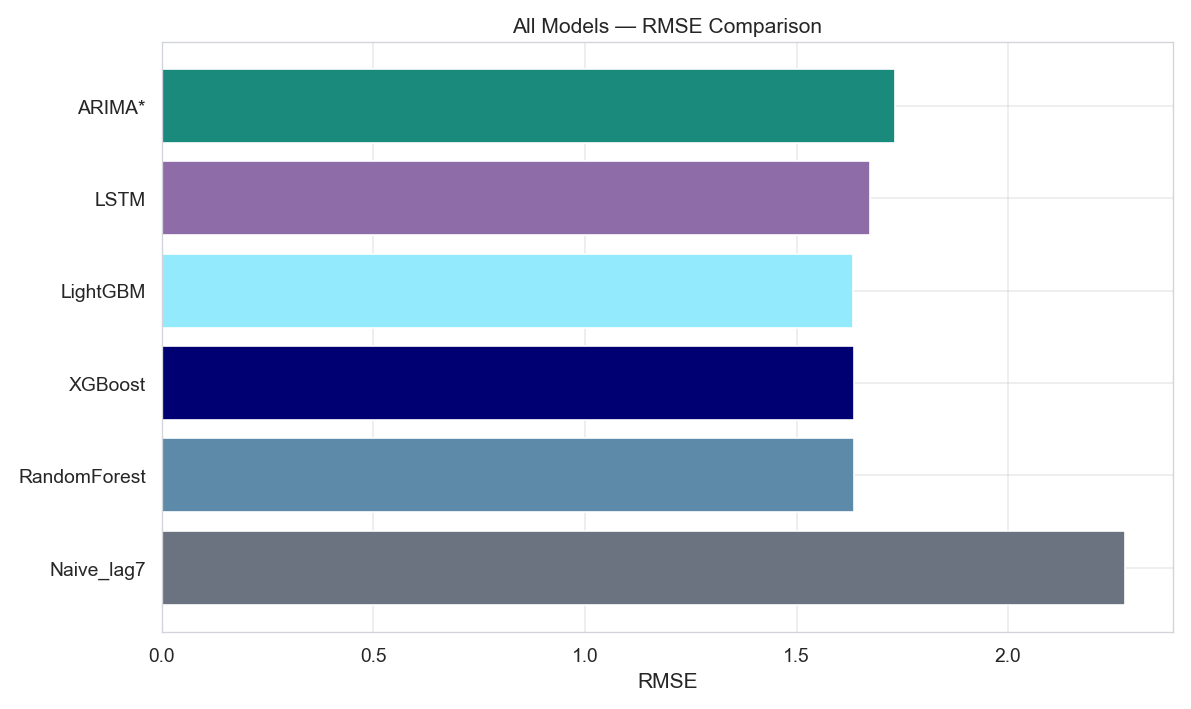
\includegraphics[width=0.85\textwidth]{figures/24_all_models_comparison.png}
\caption{Comparison of forecast accuracy (RMSE) across all six models. The three tree-based models form a tight cluster, substantially outperforming both classical and deep learning alternatives.}
\label{fig:all_models_comparison}
\end{figure}

ARIMA and LSTM occupy an intermediate position: both significantly outperform the naive baseline (RMSE reductions of 28.2\% and 27.7\% respectively) but fall short of the tree-based models. This result is consistent with the findings of the M5 forecasting competition \citep{makridakis2021m5findings}, where gradient boosting algorithms consistently outperformed both classical statistical methods and standalone deep learning approaches. The LSTM's slightly lower MAPE (49.8\%) but higher RMSE suggests it handles the zero-heavy distribution differently from tree models, producing fewer large percentage errors but occasionally larger absolute deviations.

\subsection{Comparison of Results Across Models}

\textbf{Promotional vs. non-promotional performance.} Table~\ref{tab:promo_results} compares model performance across demand segments:

\begin{table}[H]
\centering
\small
\caption{Model performance by demand segment (last validation fold).}
\label{tab:promo_results}
\begin{tabular}{|l|l|r|r|r|r|}
\hline
\textbf{Segment} & \textbf{Model} & \textbf{MAE} & \textbf{RMSE} & \textbf{MAPE (\%)} & \textbf{$\sigma_e$} \\
\hline
\multirow{4}{*}{Non-Promo} & XGBoost & 1.299 & 2.055 & 52.3 & 2.055 \\
 & LightGBM & 1.308 & 2.058 & 51.8 & 2.058 \\
 & Random Forest & 1.327 & 2.073 & 51.6 & 2.073 \\
 & Naive (lag-7) & 1.565 & 2.969 & 85.9 & 2.969 \\
\hline
\multirow{4}{*}{Promo} & XGBoost & 1.917 & 2.844 & 51.7 & 2.836 \\
 & LightGBM & 1.911 & 2.851 & 51.4 & 2.838 \\
 & Random Forest & 1.944 & 2.884 & 51.6 & 2.873 \\
 & Naive (lag-7) & 2.448 & 3.956 & 86.9 & 3.955 \\
\hline
\end{tabular}
\end{table}

Promotional demand is consistently harder to predict across all models, with RMSE values approximately 38\% higher than for non-promotional periods. However, the ML models maintain their advantage over the naive baseline in both segments, with RMSE improvements of approximately 28\% for non-promotional and 28\% for promotional demand.

\textbf{Per-product RMSE distribution.} Analysis at the individual product level reveals that LightGBM achieves a median per-product RMSE of 1.65, compared to 2.36 for the naive baseline. The improvement is not uniform: some products see RMSE reductions exceeding 15 units, while approximately 10 products show marginally worse performance with ML than with the naive approach. These products tend to have very low and stable demand where the simple lag-7 heuristic is already near-optimal.

\begin{figure}[H]
\centering
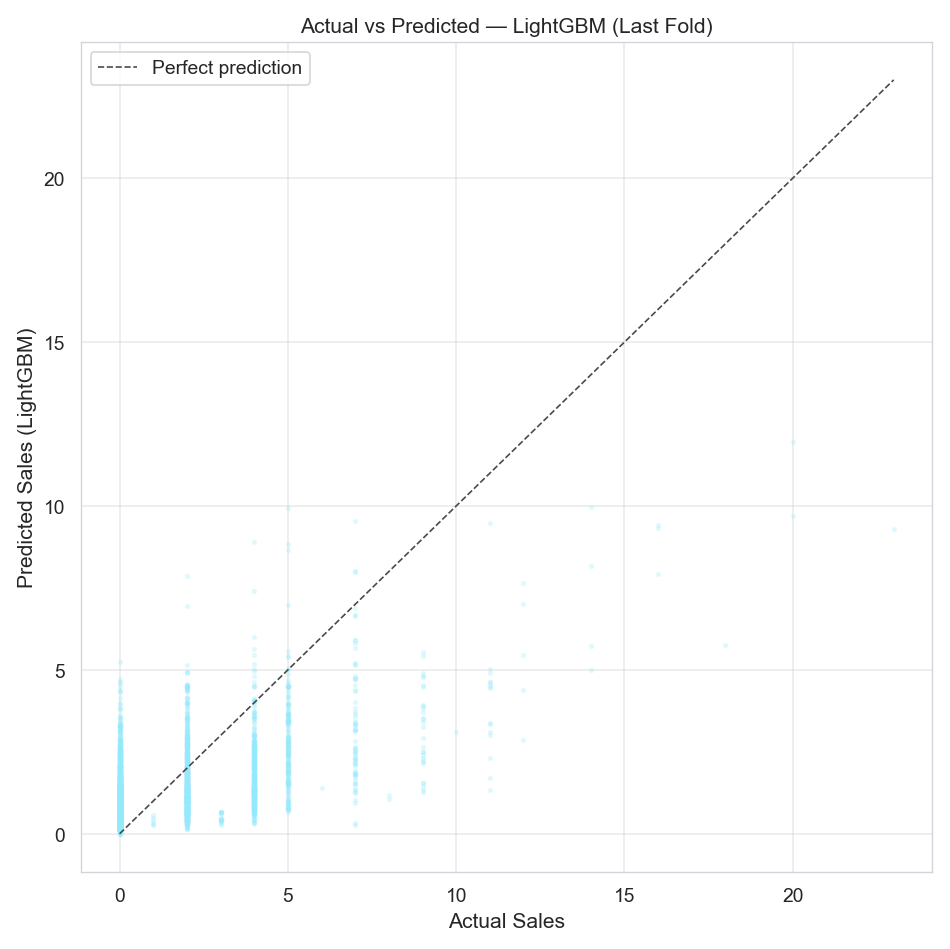
\includegraphics[width=0.85\textwidth]{figures/13_actual_vs_predicted_lgbm.png}
\caption{Actual vs.\ predicted sales for LightGBM on a sample of products. Points near the diagonal indicate accurate predictions; the cluster near the origin reflects the high proportion of zero-demand observations.}
\label{fig:actual_vs_predicted}
\end{figure}

\begin{figure}[H]
\centering
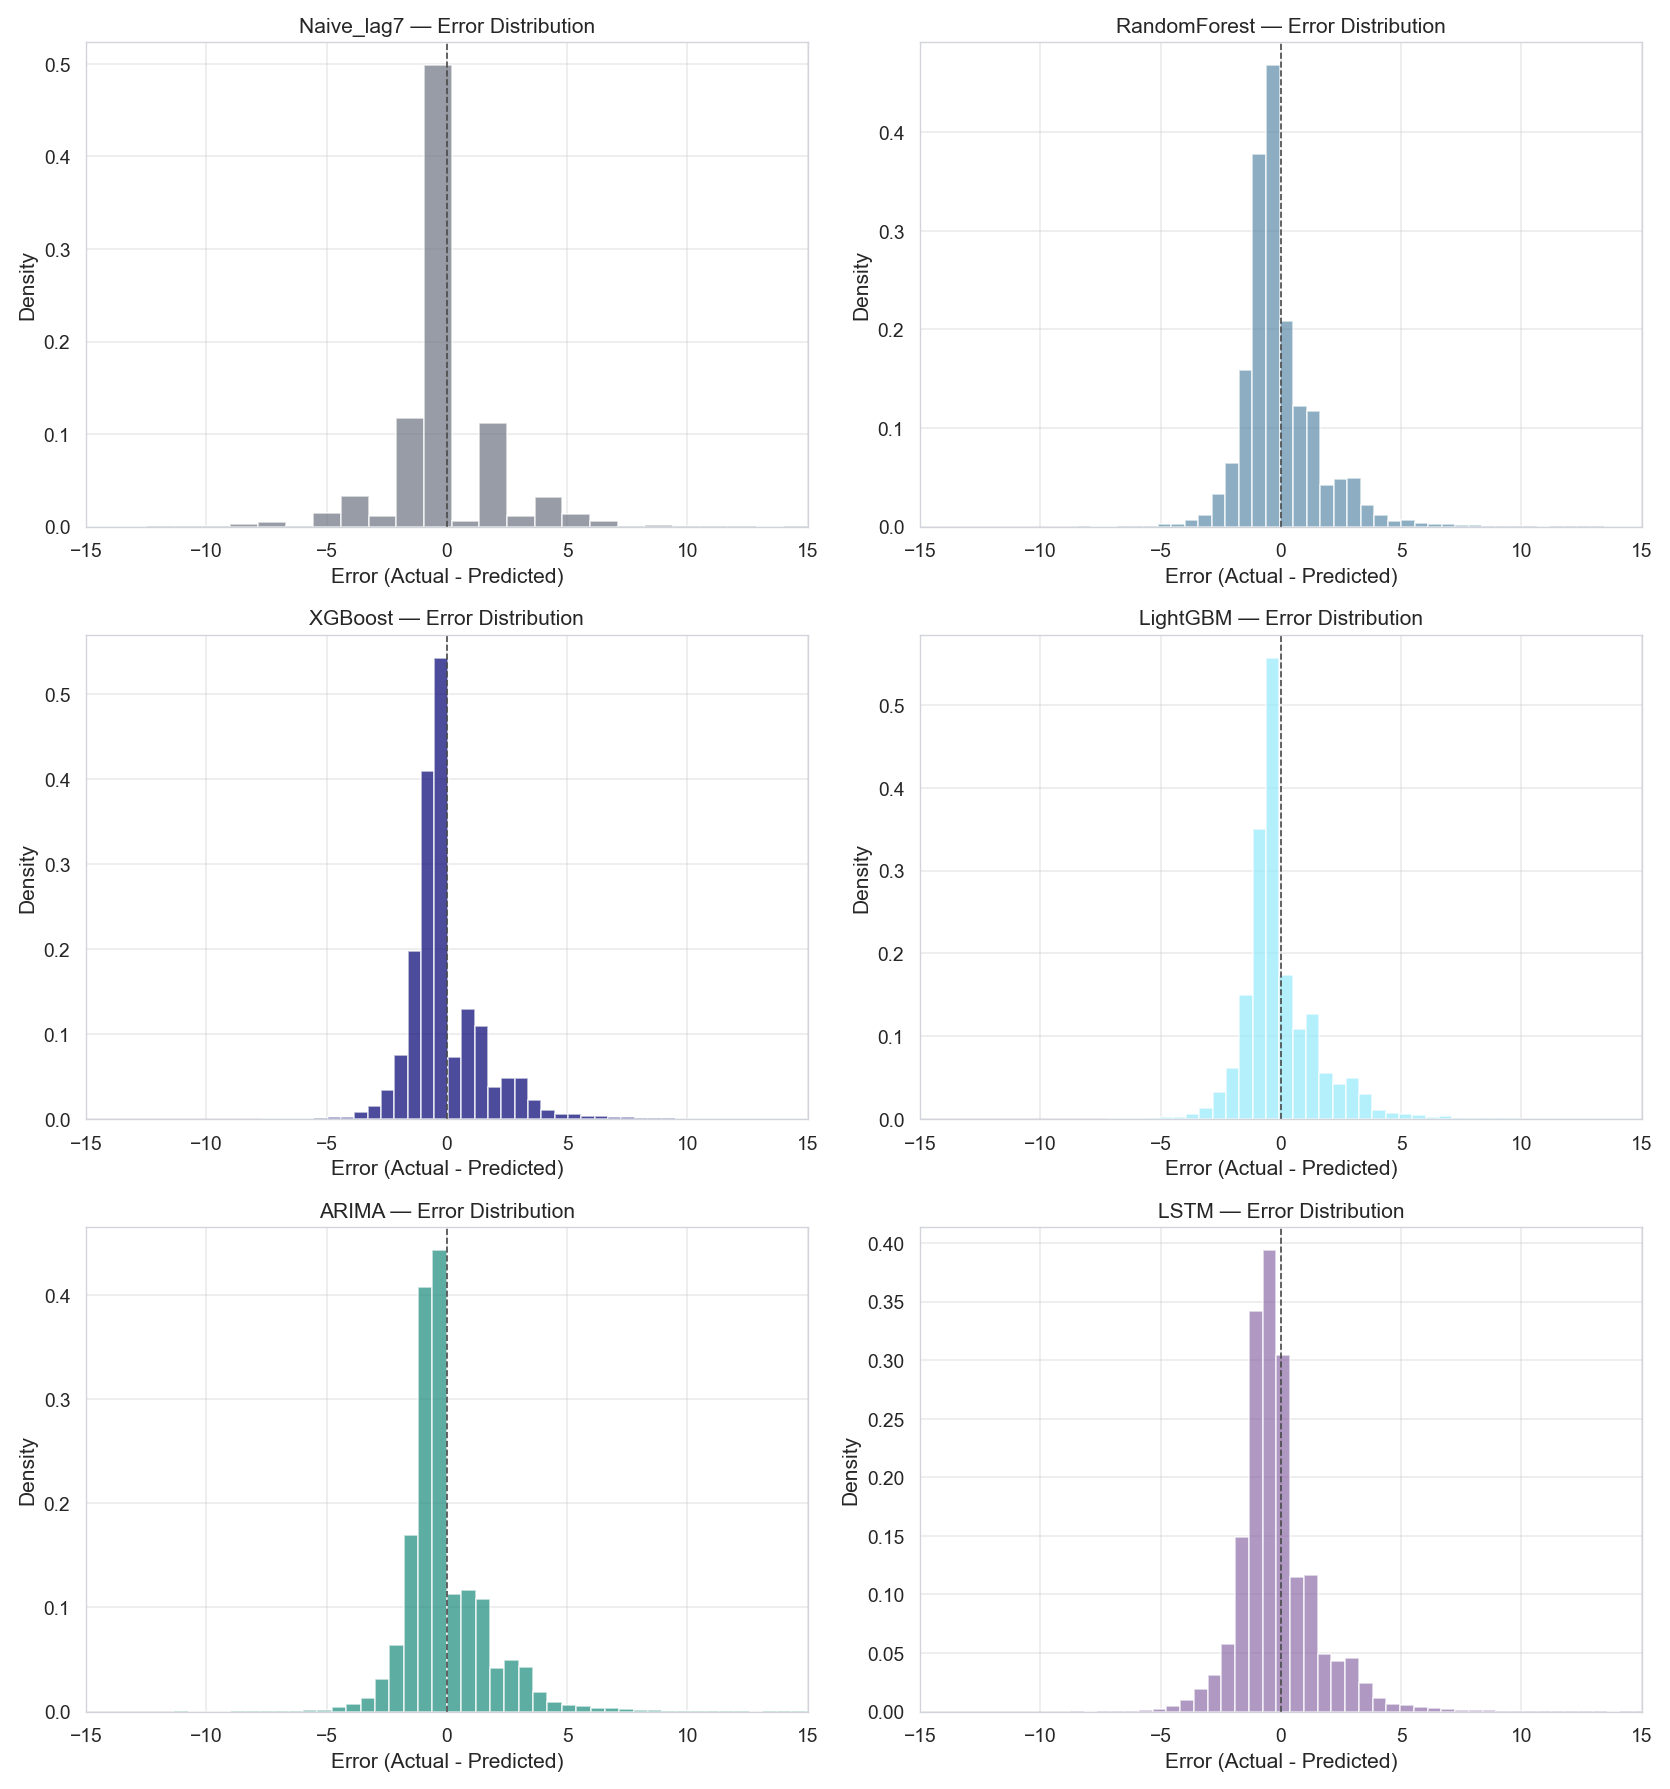
\includegraphics[width=0.85\textwidth]{figures/17_error_distributions.png}
\caption{Distribution of forecast errors by model. The ML models produce tighter, more symmetric error distributions compared to the naive baseline.}
\label{fig:error_distributions}
\end{figure}

\begin{figure}[H]
\centering
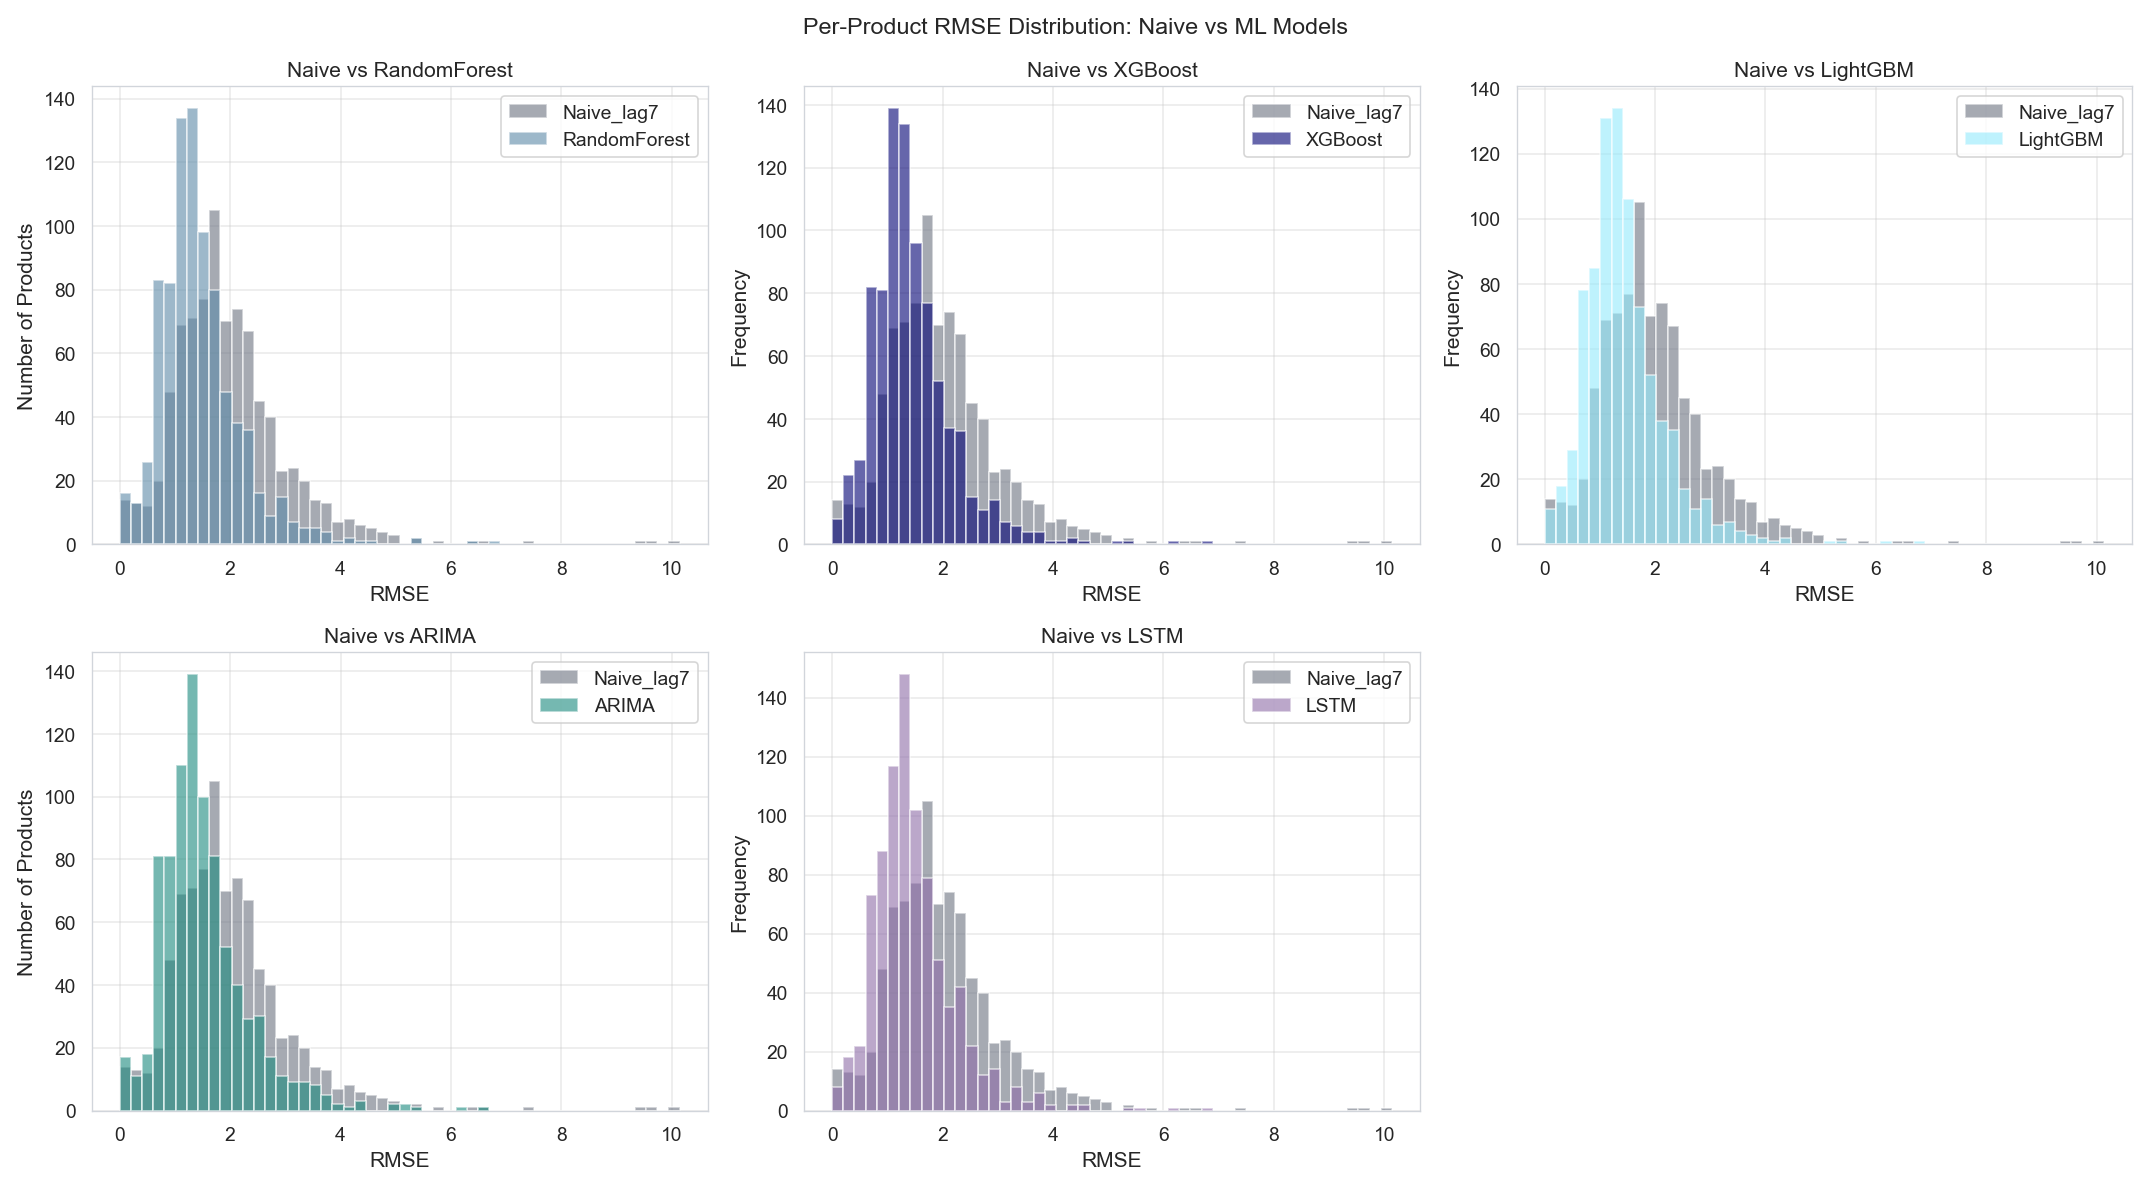
\includegraphics[width=0.85\textwidth]{figures/18_per_product_rmse_dist.png}
\caption{Distribution of per-product RMSE values. The ML models shift the distribution towards lower RMSE values compared to the naive baseline.}
\label{fig:per_product_rmse}
\end{figure}

\textbf{SHAP feature importance.} To understand the drivers of model predictions, SHAP (SHapley Additive exPlanations) analysis was performed on the LightGBM model. Table~\ref{tab:shap_top10} presents the ten most influential features:

\begin{table}[H]
\centering
\small
\caption{Top 10 features by mean absolute SHAP value (LightGBM).}
\label{tab:shap_top10}
\begin{tabular}{|r|l|r|}
\hline
\textbf{Rank} & \textbf{Feature} & \textbf{Mean $|$SHAP$|$} \\
\hline
1 & ewma\_28 & 0.524 \\
2 & bolHoliday & 0.295 \\
3 & roll\_mean\_28 & 0.150 \\
4 & day\_of\_week & 0.079 \\
5 & udsStock & 0.063 \\
6 & roll\_max\_28 & 0.046 \\
7 & lag\_28 & 0.025 \\
8 & bolOpen & 0.022 \\
9 & roll\_mean\_14 & 0.017 \\
10 & roll\_max\_14 & 0.016 \\
\hline
\end{tabular}
\end{table}

The 28-day EWMA emerges as the single most important predictor, followed by the holiday indicator and the 28-day rolling mean. This confirms that the model relies heavily on smoothed representations of recent demand history, with calendar effects providing secondary but significant predictive power. Notably, the longer-horizon features (28-day windows) dominate over shorter-horizon ones (7-day), suggesting that the model captures medium-term demand trends rather than relying solely on short-term momentum.

\begin{figure}[H]
\centering
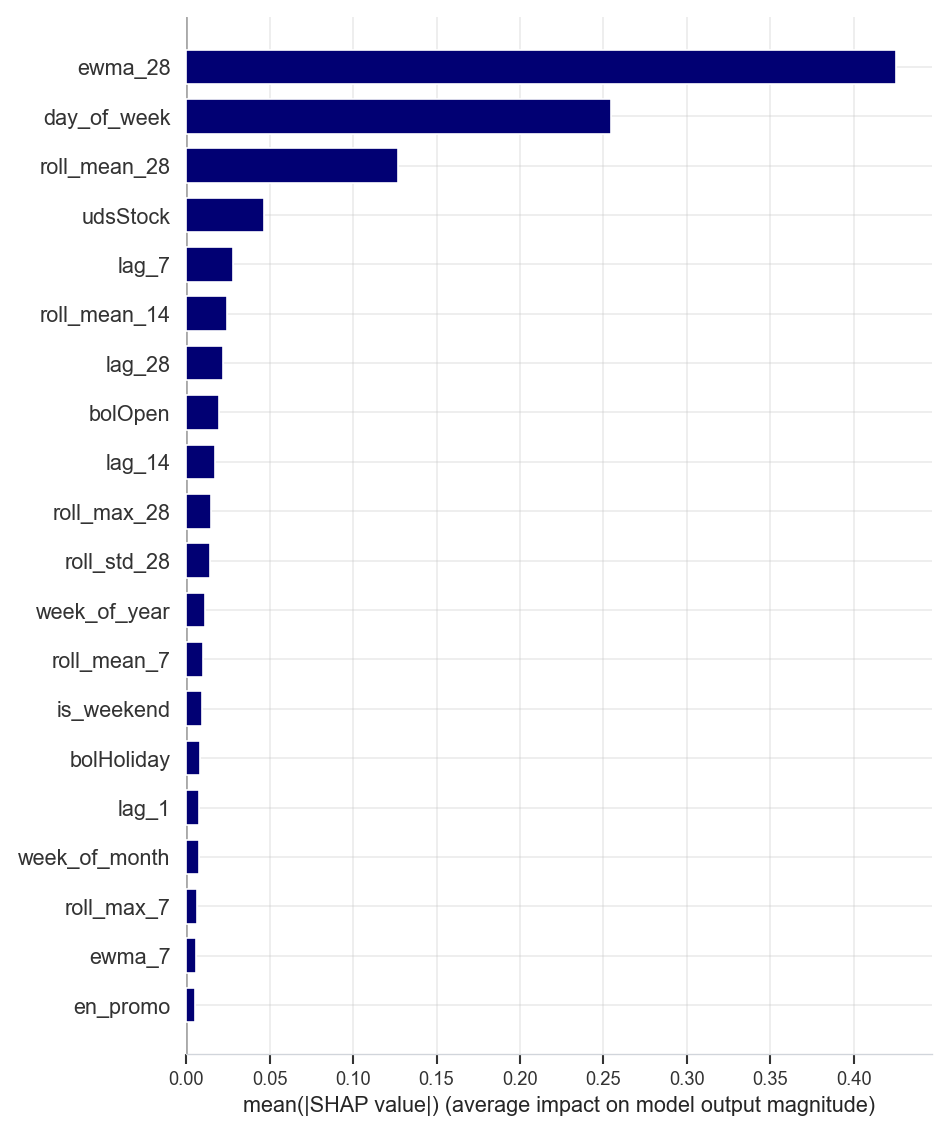
\includegraphics[width=0.85\textwidth]{figures/15_shap_bar.png}
\caption{SHAP feature importance (mean absolute SHAP values) for LightGBM. The 28-day EWMA dominates, followed by calendar and rolling statistics features.}
\label{fig:shap_bar}
\end{figure}

\begin{figure}[H]
\centering
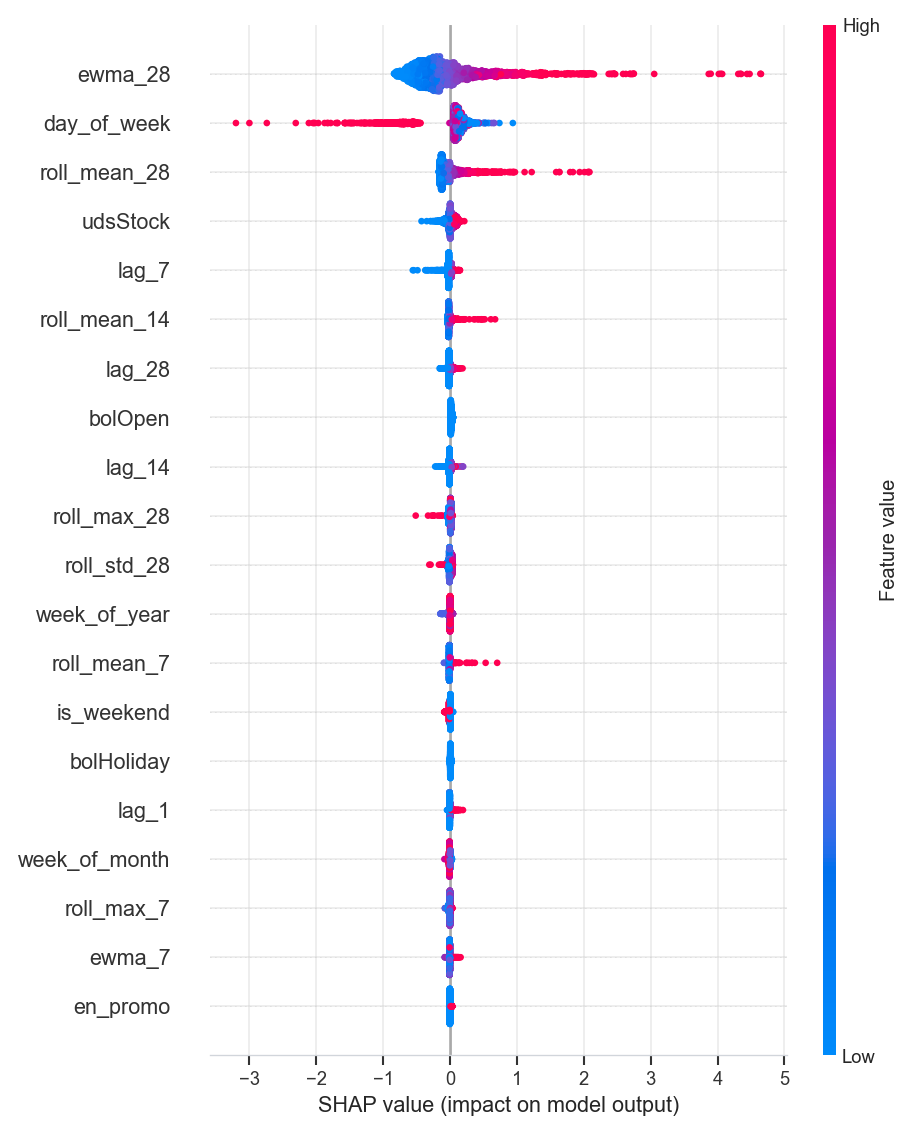
\includegraphics[width=0.85\textwidth]{figures/14_shap_summary.png}
\caption{SHAP summary plot showing the direction and magnitude of feature effects. Red indicates high feature values; blue indicates low values. High \texttt{ewma\_28} values push predictions upward, consistent with higher recent demand leading to higher forecasts.}
\label{fig:shap_summary}
\end{figure}

\subsection{Conclusions from Results}

The evaluation yields several key findings:

\begin{enumerate}
    \item The three tree-based machine learning models (XGBoost, LightGBM, Random Forest) achieve the best performance, with RMSE values within 1\% of each other. This suggests that the feature engineering, rather than the specific algorithm choice, is the primary driver of forecast quality among this model family.

    \item ARIMA and LSTM occupy an intermediate tier, both significantly outperforming the naive baseline (RMSE reductions of 28\% and 28\% respectively) but falling short of the tree-based models. ARIMA's per-product fitting captures local demand patterns effectively but cannot leverage cross-product information or engineered features. LSTM captures sequential dependencies but requires substantially more training data and computation to match tree-based performance.

    \item The improvement over the naive baseline is substantial across all ML approaches (28--30\% RMSE reduction), demonstrating the value of incorporating engineered features and systematic model training over simple heuristic forecasting.

    \item Promotional demand remains the most challenging segment, with RMSE approximately 38\% higher than non-promotional demand across all models. However, the ML models maintain their relative advantage over the baseline in both segments.

    \item SHAP analysis reveals that smoothed demand history (EWMA and rolling statistics) and calendar features are the most influential predictors, validating the feature engineering strategy adopted in this work.

    \item The forecast error standard deviation ($\sigma_e \approx 2.15$ for the best tree models, $\sigma_e \approx 2.22$ for ARIMA/LSTM, compared to $\sigma_e \approx 3.09$ for the naive baseline) translates directly into safety stock reductions, as quantified in the following section.
\end{enumerate}


\section{Impact of Algorithm Improvement}

\subsection{Impact on Processes}

The transition from a naive forecasting approach to machine learning models has implications beyond numerical accuracy improvements. From an operational perspective, the key process impacts are:

\textbf{Safety stock reduction.} Using the safety stock formulation from Equation~\ref{eq:safety_stock} with a 95\% service level ($z = 1.645$) and a protection period of 10 days (3 days lead time + 7 days review period), the total safety stock across all 894 products decreases from 11,953 units under the naive forecast to 8,276 units under LightGBM --- a reduction of 30.8\%. This means that the same service level can be maintained with significantly less inventory investment.

\textbf{Forecast error symmetry.} Analysis of error distributions shows that the ML models produce approximately symmetric errors centred near zero, whereas the naive baseline exhibits a slight positive bias (tendency to overforecast). Symmetric errors are preferable for inventory planning, as they indicate that the forecast is equally likely to overestimate or underestimate demand, allowing safety stock to function as intended.

\textbf{Sensitivity to service level.} Table~\ref{tab:sensitivity} presents the total safety stock requirements across different service levels:

\begin{table}[H]
\centering
\small
\caption{Total safety stock (units) by model and service level.}
\label{tab:sensitivity}
\begin{tabular}{|l|r|r|r|}
\hline
\textbf{Model} & \textbf{90\%} & \textbf{95\%} & \textbf{99\%} \\
\hline
LightGBM & 6,450 & 8,276 & 11,702 \\
XGBoost & 6,466 & 8,296 & 11,731 \\
Random Forest & 6,507 & 8,350 & 11,806 \\
Naive (lag-7) & 9,316 & 11,953 & 16,902 \\
\hline
\end{tabular}
\end{table}

The ML models consistently require approximately 30\% less safety stock than the naive baseline across all service levels, demonstrating that the improvement is robust and not dependent on a specific service level assumption.

\begin{figure}[H]
\centering
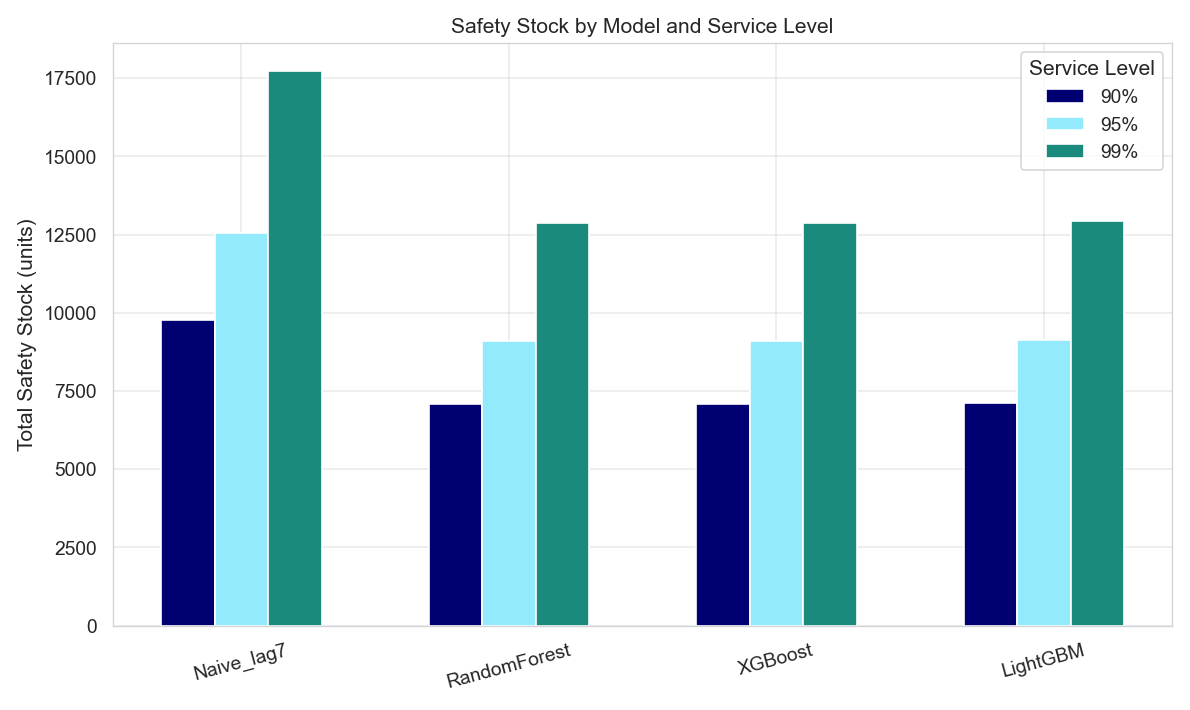
\includegraphics[width=0.85\textwidth]{figures/21_safety_stock_by_service_level.png}
\caption{Total safety stock requirements by model and service level. The ML models maintain a consistent ~30\% advantage over the naive baseline across all service levels.}
\label{fig:safety_stock_service_level}
\end{figure}

\subsection{Economic Impact}

The economic impact analysis combines two cost components: the newsvendor cost (direct cost of forecast errors) and the safety stock holding cost.

\textbf{Newsvendor cost analysis.} Following the total cost formulation from Equation~\ref{eq:total_cost}, the asymmetric costs of overforecasting and underforecasting were computed using cost parameters of $C_o = \text{\euro}0.10$ per unit per day (overage/holding) and $C_u = \text{\euro}0.50$ per unit per day (underage/lost sale), yielding a critical ratio of 0.83. These values reflect a typical retail/industrial setting where stockout costs substantially exceed holding costs.

Table~\ref{tab:newsvendor} presents the newsvendor cost results:

\begin{table}[H]
\centering
\small
\caption{Newsvendor cost analysis (30-day test period, annualised).}
\label{tab:newsvendor}
\begin{tabular}{|l|r|r|r|r|}
\hline
\textbf{Model} & \textbf{Overage (€)} & \textbf{Underage (€)} & \textbf{Total (€)} & \textbf{Annual est. (€)} \\
\hline
Naive (lag-7) & 2,227 & 11,138 & 13,365 & 162,603 \\
Random Forest & 1,830 & 9,538 & 11,367 & 138,304 \\
LightGBM & 1,786 & 9,489 & 11,275 & 137,182 \\
XGBoost & 1,785 & 9,392 & 11,176 & 135,979 \\
\hline
\end{tabular}
\end{table}

XGBoost achieves the lowest newsvendor cost, saving approximately \euro26,600 annually (16.4\%) compared to the naive baseline. Underage costs dominate in all models, consistent with the asymmetric cost structure where stockouts are five times more expensive than excess inventory.

\textbf{Combined cost analysis.} Table~\ref{tab:combined_cost} presents the total annual cost combining newsvendor costs with safety stock holding costs at the 95\% service level:

\begin{table}[H]
\centering
\small
\caption{Combined annual cost: newsvendor + safety stock holding (95\% service level).}
\label{tab:combined_cost}
\begin{tabular}{|l|r|r|r|}
\hline
\textbf{Model} & \textbf{Newsvendor (€/yr)} & \textbf{SS Holding (€/yr)} & \textbf{Total (€/yr)} \\
\hline
Naive (lag-7) & 162,603 & 436,294 & 598,896 \\
Random Forest & 138,304 & 304,763 & 443,067 \\
LightGBM & 137,182 & 302,083 & 439,265 \\
XGBoost & 135,979 & 302,816 & 438,796 \\
\hline
\end{tabular}
\end{table}

The ML models achieve total annual cost savings of approximately \euro160,000 (26.7\%) compared to the naive baseline. XGBoost and LightGBM perform nearly identically in economic terms, with XGBoost holding a marginal advantage of \euro469 annually.

\begin{figure}[H]
\centering
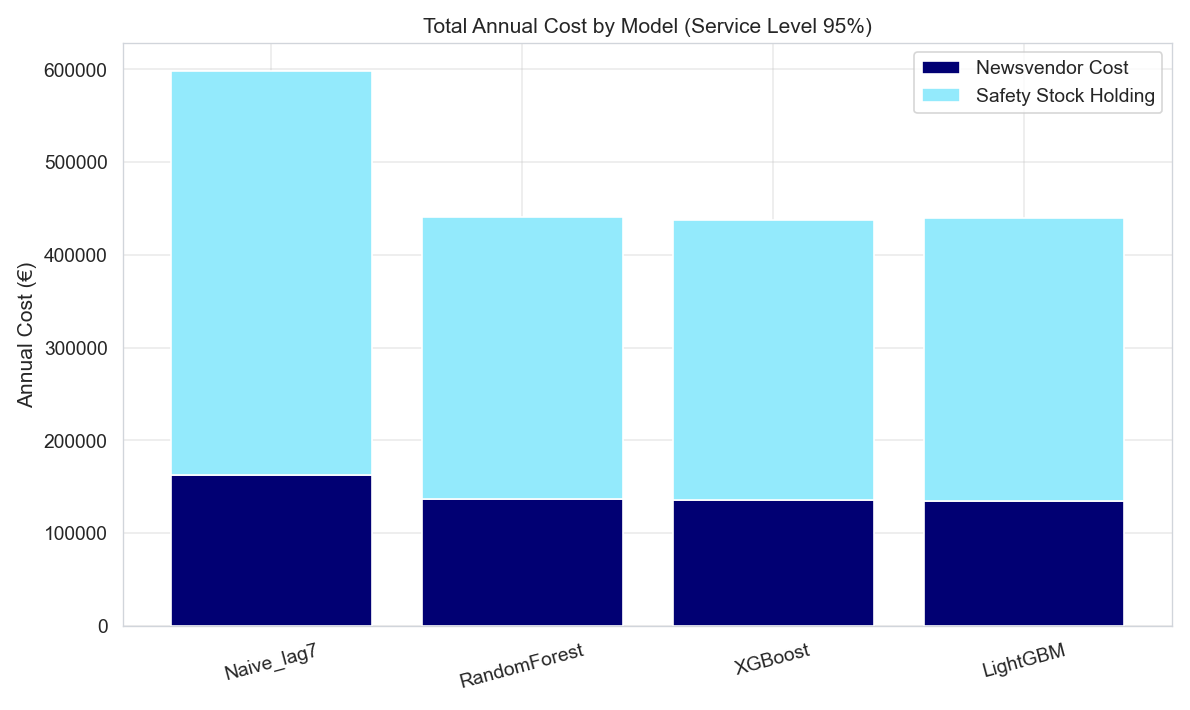
\includegraphics[width=0.85\textwidth]{figures/22_combined_annual_cost.png}
\caption{Combined annual inventory cost (newsvendor + safety stock holding) by model. The ML models reduce total costs by approximately 26.7\% compared to the naive baseline.}
\label{fig:combined_annual_cost}
\end{figure}

These results demonstrate that the forecast accuracy improvements documented in Section~3.6 translate into meaningful economic benefits. The 28\% reduction in RMSE corresponds to a 26.7\% reduction in total inventory-related costs, confirming the theoretical relationship between forecast error and inventory costs established in Chapter~2 (Equations~\ref{eq:ss_cost} and \ref{eq:total_cost}).

It is important to note that the cost parameters used in this analysis ($C_o$ and $C_u$) are illustrative values chosen to reflect typical industrial cost structures. The relative ranking of models and the percentage savings are robust to reasonable variations in these parameters, as the underlying driver is the reduction in forecast error rather than the specific cost assumptions. A sensitivity analysis across service levels (Table~\ref{tab:sensitivity}) confirms that the ML advantage is maintained regardless of the risk tolerance adopted by the organisation.
 in TFM_onamas.tex

This chapter presents the complete design and implementation of the demand forecasting system, following the CRISP-DM methodology introduced in Chapter~1. The work progresses from data acquisition and exploration through preprocessing, feature engineering, model development, evaluation, and finally the economic impact analysis that connects forecast accuracy to inventory cost savings.

\section{Data Origin}

\subsection{Data Acquisition}

The dataset used in this project was provided by the thesis supervisor and corresponds to real historical data from a company operating in the automotive sector. The data covers daily demand records for a portfolio of products, along with supplementary information on calendar events, promotional campaigns, and stock levels. All data was received in a single Microsoft Excel file (\texttt{Datos.xlsx}) containing four sheets, each representing a distinct dimension of the business context.

No personally identifiable information is present in the dataset, and all product references are anonymised using numerical identifiers, ensuring compliance with data privacy requirements as discussed in Section~\ref{s:etic}.

\subsection{Data Description}

The dataset comprises four tables, summarised in Table~\ref{tab:data_sheets}:

\begin{table}[H]
\centering
\small
\caption{Structure of the source dataset (\texttt{Datos.xlsx}).}
\label{tab:data_sheets}
\begin{tabular}{|l|l|r|p{5.5cm}|}
\hline
\textbf{Sheet} & \textbf{Key columns} & \textbf{Rows} & \textbf{Description} \\
\hline
Ventas (Sales) & producto, fecha, udsVenta & 654,588 & Daily unit sales per product \\
\hline
Calendario & fecha, bolOpen, bolHoliday & 732 & Calendar flags: business day and holiday indicators \\
\hline
Promociones & producto, fechaInicio, fechaFin & 1,894 & Promotional campaign periods per product \\
\hline
Stock & producto, fecha, udsStock & 654,588 & Daily stock levels per product \\
\hline
\end{tabular}
\end{table}

The sales sheet constitutes the core of the dataset, containing 654,588 daily observations across 894 unique products over a period of 732 days, spanning from November 2022 to November 2024. Each record represents the number of units sold for a specific product on a specific date.

The calendar sheet provides 732 daily records with two binary indicators: \texttt{bolOpen} (whether the business was open) and \texttt{bolHoliday} (whether the date was a public holiday). The promotions sheet contains 1,894 records defining promotional campaign windows through start and end dates for each product. The stock sheet mirrors the sales structure, recording the closing stock level for each product-date combination.

\subsection{Data Loading}

All four sheets were loaded into memory using the \texttt{pandas} library with the \texttt{openpyxl} engine. The sales and stock tables were merged on the shared keys \texttt{(producto, fecha)}, and the calendar information was joined on \texttt{fecha}. Promotional periods were transformed from date ranges into a binary indicator (\texttt{en\_promo}) at the product-date level, marking each observation as promotional or non-promotional based on whether the date fell within any active campaign for that product.

After merging, the resulting dataset contained 654,588 rows and served as the foundation for all subsequent analysis. The merged dataset was persisted in Apache Parquet format for efficient reloading in downstream scripts.


\section{Data Exploration}

\subsection{Data Summary}

An initial statistical summary of the target variable (\texttt{udsVenta}, units sold) revealed a highly skewed distribution. The mean daily sales per product were 1.42 units, with a median of zero and a standard deviation of 3.56. The maximum observed value was 99 units. This distribution reflects the nature of automotive parts demand, where the majority of product-day combinations register zero sales, punctuated by occasional larger orders.

Table~\ref{tab:sales_stats} presents the key descriptive statistics:

\begin{table}[H]
\centering
\small
\caption{Descriptive statistics of daily unit sales (\texttt{udsVenta}).}
\label{tab:sales_stats}
\begin{tabular}{|l|r|}
\hline
\textbf{Statistic} & \textbf{Value} \\
\hline
Count & 654,588 \\
Mean & 1.42 \\
Std. deviation & 3.56 \\
Median (50\%) & 0.00 \\
75th percentile & 1.00 \\
95th percentile & 7.00 \\
Maximum & 99 \\
Zero-sales proportion & 64.5\% \\
\hline
\end{tabular}
\end{table}

The high proportion of zero-sales observations (64.5\%) is a defining characteristic of this dataset and has important implications for model selection and evaluation, as discussed in subsequent sections.

\begin{figure}[H]
\centering
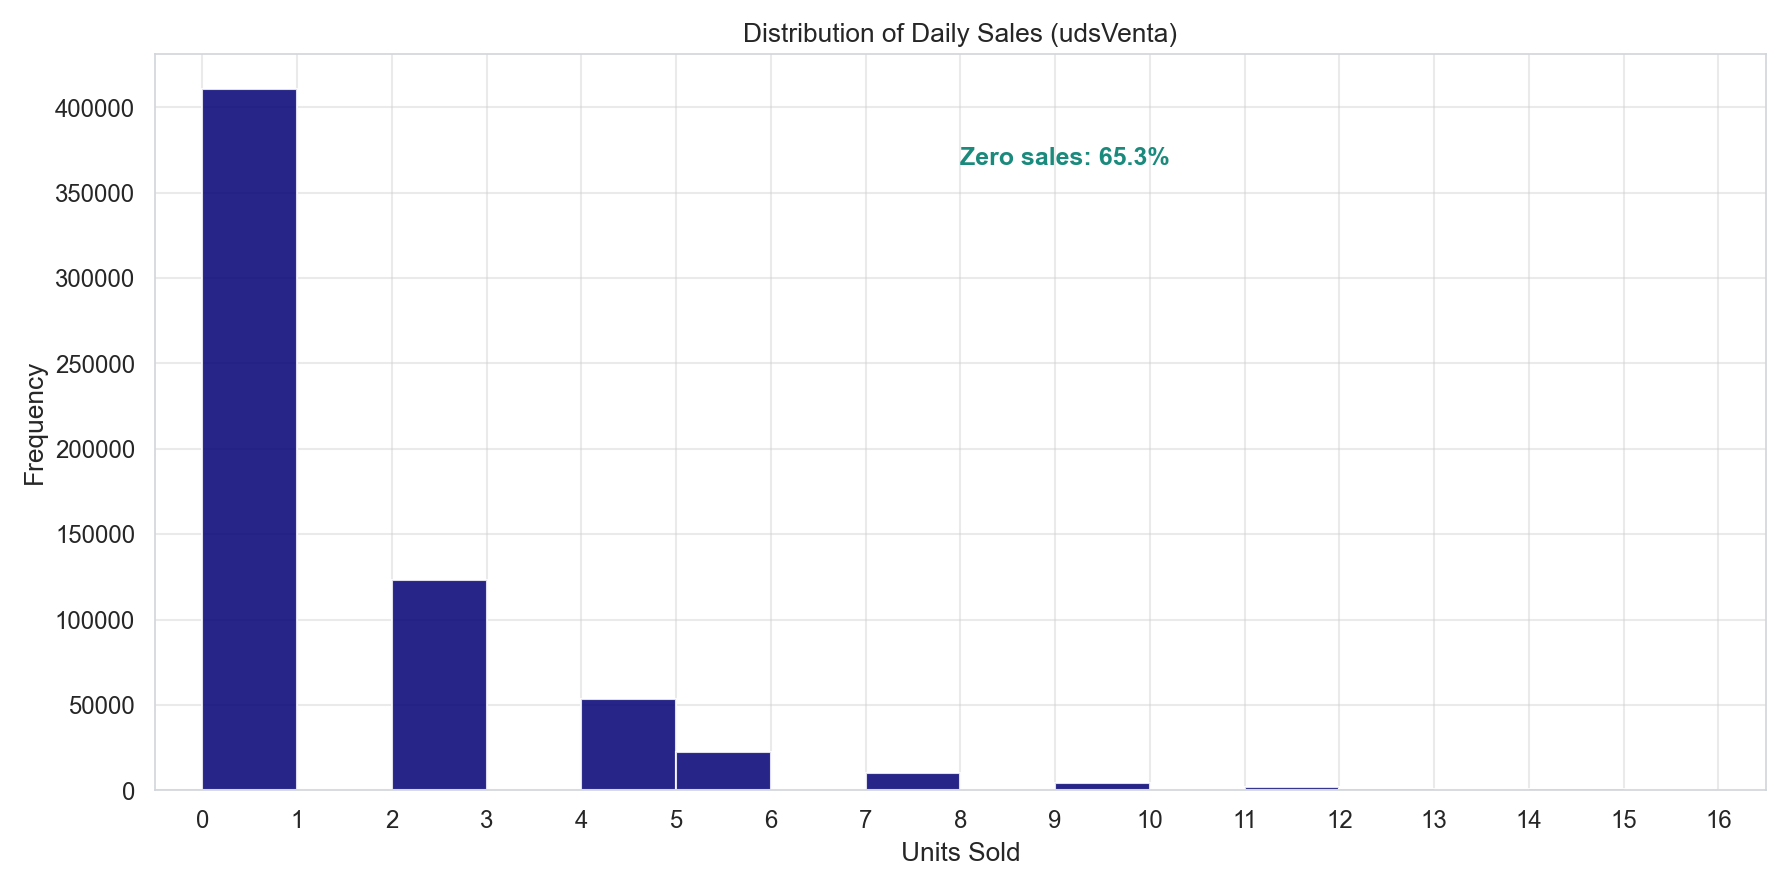
\includegraphics[width=0.85\textwidth]{figures/01_sales_distribution.png}
\caption{Distribution of daily unit sales (\texttt{udsVenta}). The histogram confirms the extreme right skew, with the majority of observations at zero.}
\label{fig:sales_distribution}
\end{figure}

\subsection{Statistical Analysis}

The exploratory analysis examined demand patterns across several dimensions:

\textbf{Day-of-week patterns.} Sales exhibit a clear weekly cycle, with the highest volumes on weekdays (Monday through Friday) and a sharp decline on Saturdays. Sunday sales are near zero, consistent with the business being closed on Sundays as indicated by the \texttt{bolOpen} calendar flag. This weekly seasonality motivates the inclusion of day-of-week features and the use of a lag-7 naive baseline (same weekday, previous week) as the primary benchmark.

\begin{figure}[H]
\centering
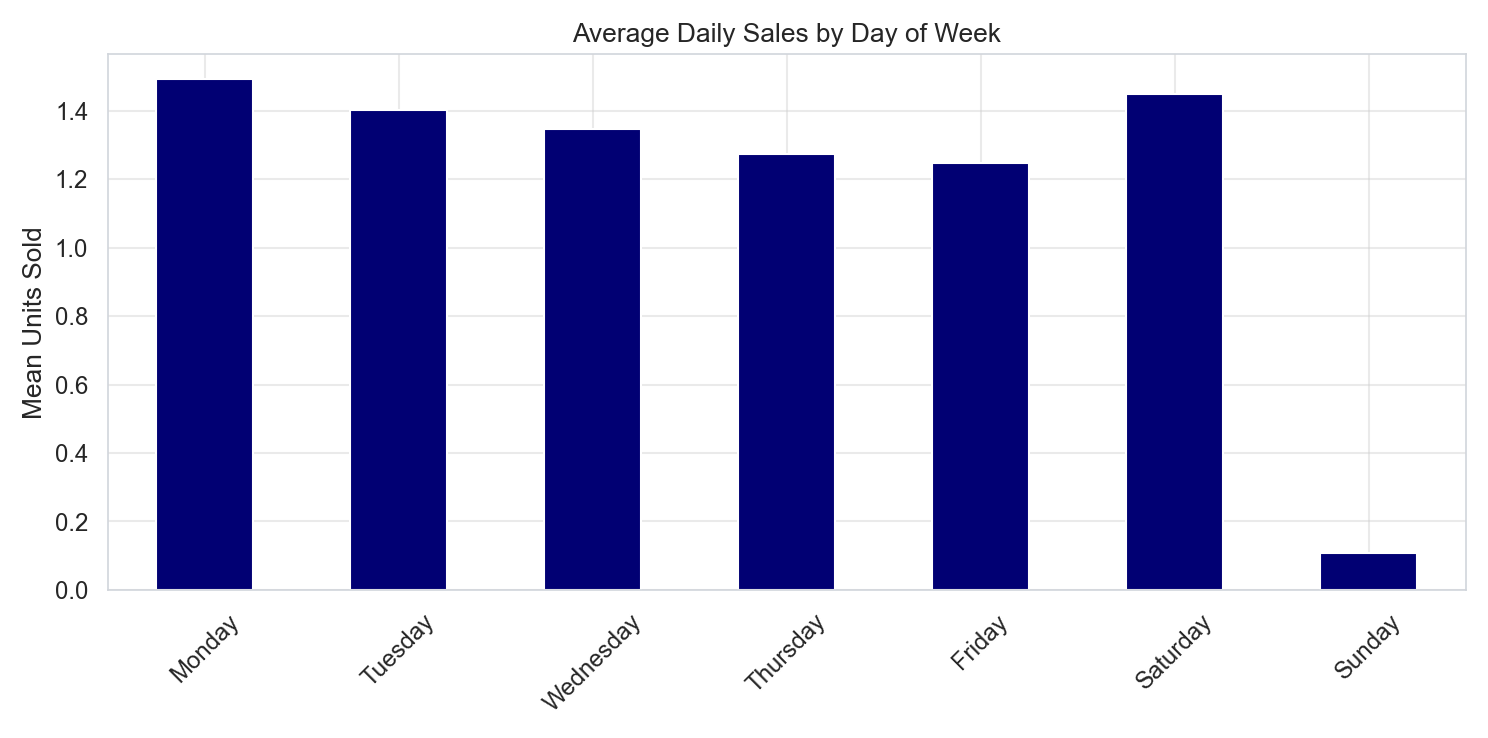
\includegraphics[width=0.85\textwidth]{figures/02_sales_by_day_of_week.png}
\caption{Average daily sales by day of the week. The weekly cycle is clearly visible, with near-zero sales on Sundays.}
\label{fig:sales_by_dow}
\end{figure}

\textbf{Monthly and seasonal patterns.} Monthly aggregated sales show moderate variation across the year, without a single dominant seasonal peak. However, certain months consistently show higher activity, suggesting that calendar-based features (month, week of year) may contribute predictive value.

\textbf{Promotional effects.} Comparing sales during promotional and non-promotional periods revealed that mean sales during promotions (1.83 units) were slightly higher than during non-promotional periods (1.38 units). However, the difference is modest, and the promotional flag alone does not capture the full complexity of promotional demand dynamics, which motivated the engineering of additional promotional features described in Section~3.4.

\begin{figure}[H]
\centering
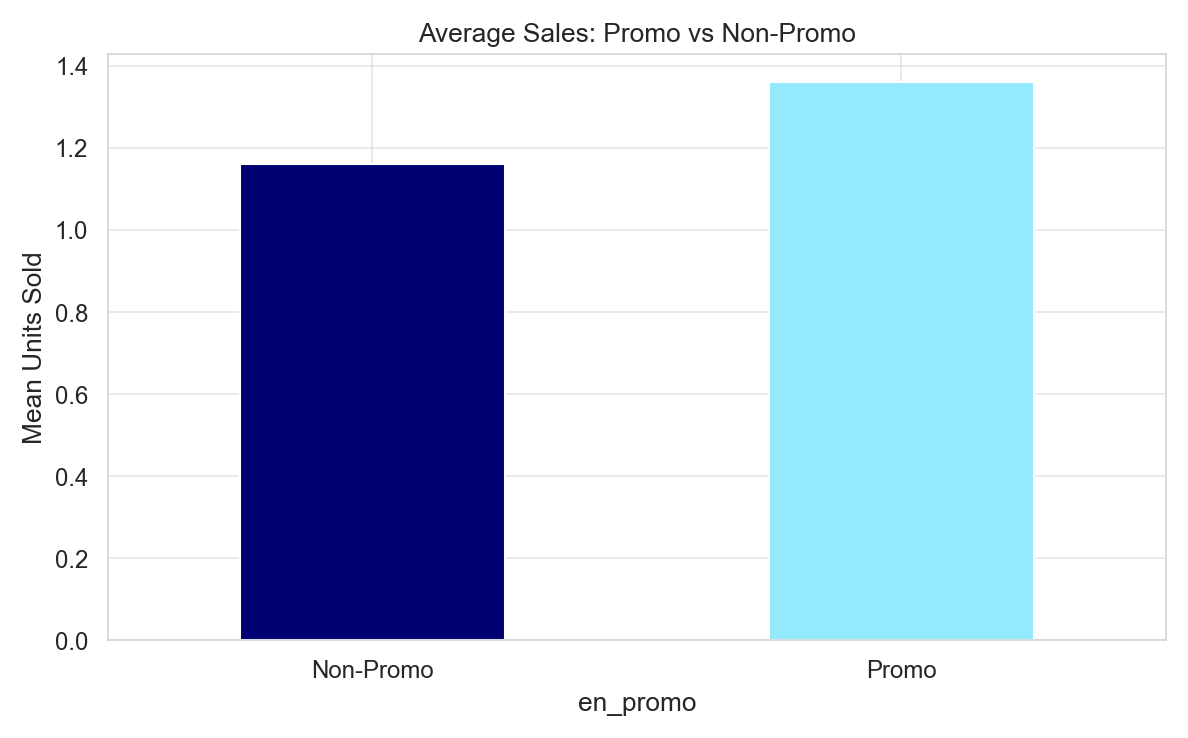
\includegraphics[width=0.85\textwidth]{figures/05_promo_vs_nonpromo.png}
\caption{Comparison of sales distributions during promotional and non-promotional periods.}
\label{fig:promo_vs_nonpromo}
\end{figure}

\textbf{Autocorrelation structure.} Autocorrelation analysis on a sample of products confirmed significant positive autocorrelation at lags 1, 7, 14, and 28, with the strongest signal at lag 7 (weekly periodicity). This finding directly supports the creation of lag features at these intervals and validates the choice of lag-7 as the naive baseline.

\begin{figure}[H]
\centering
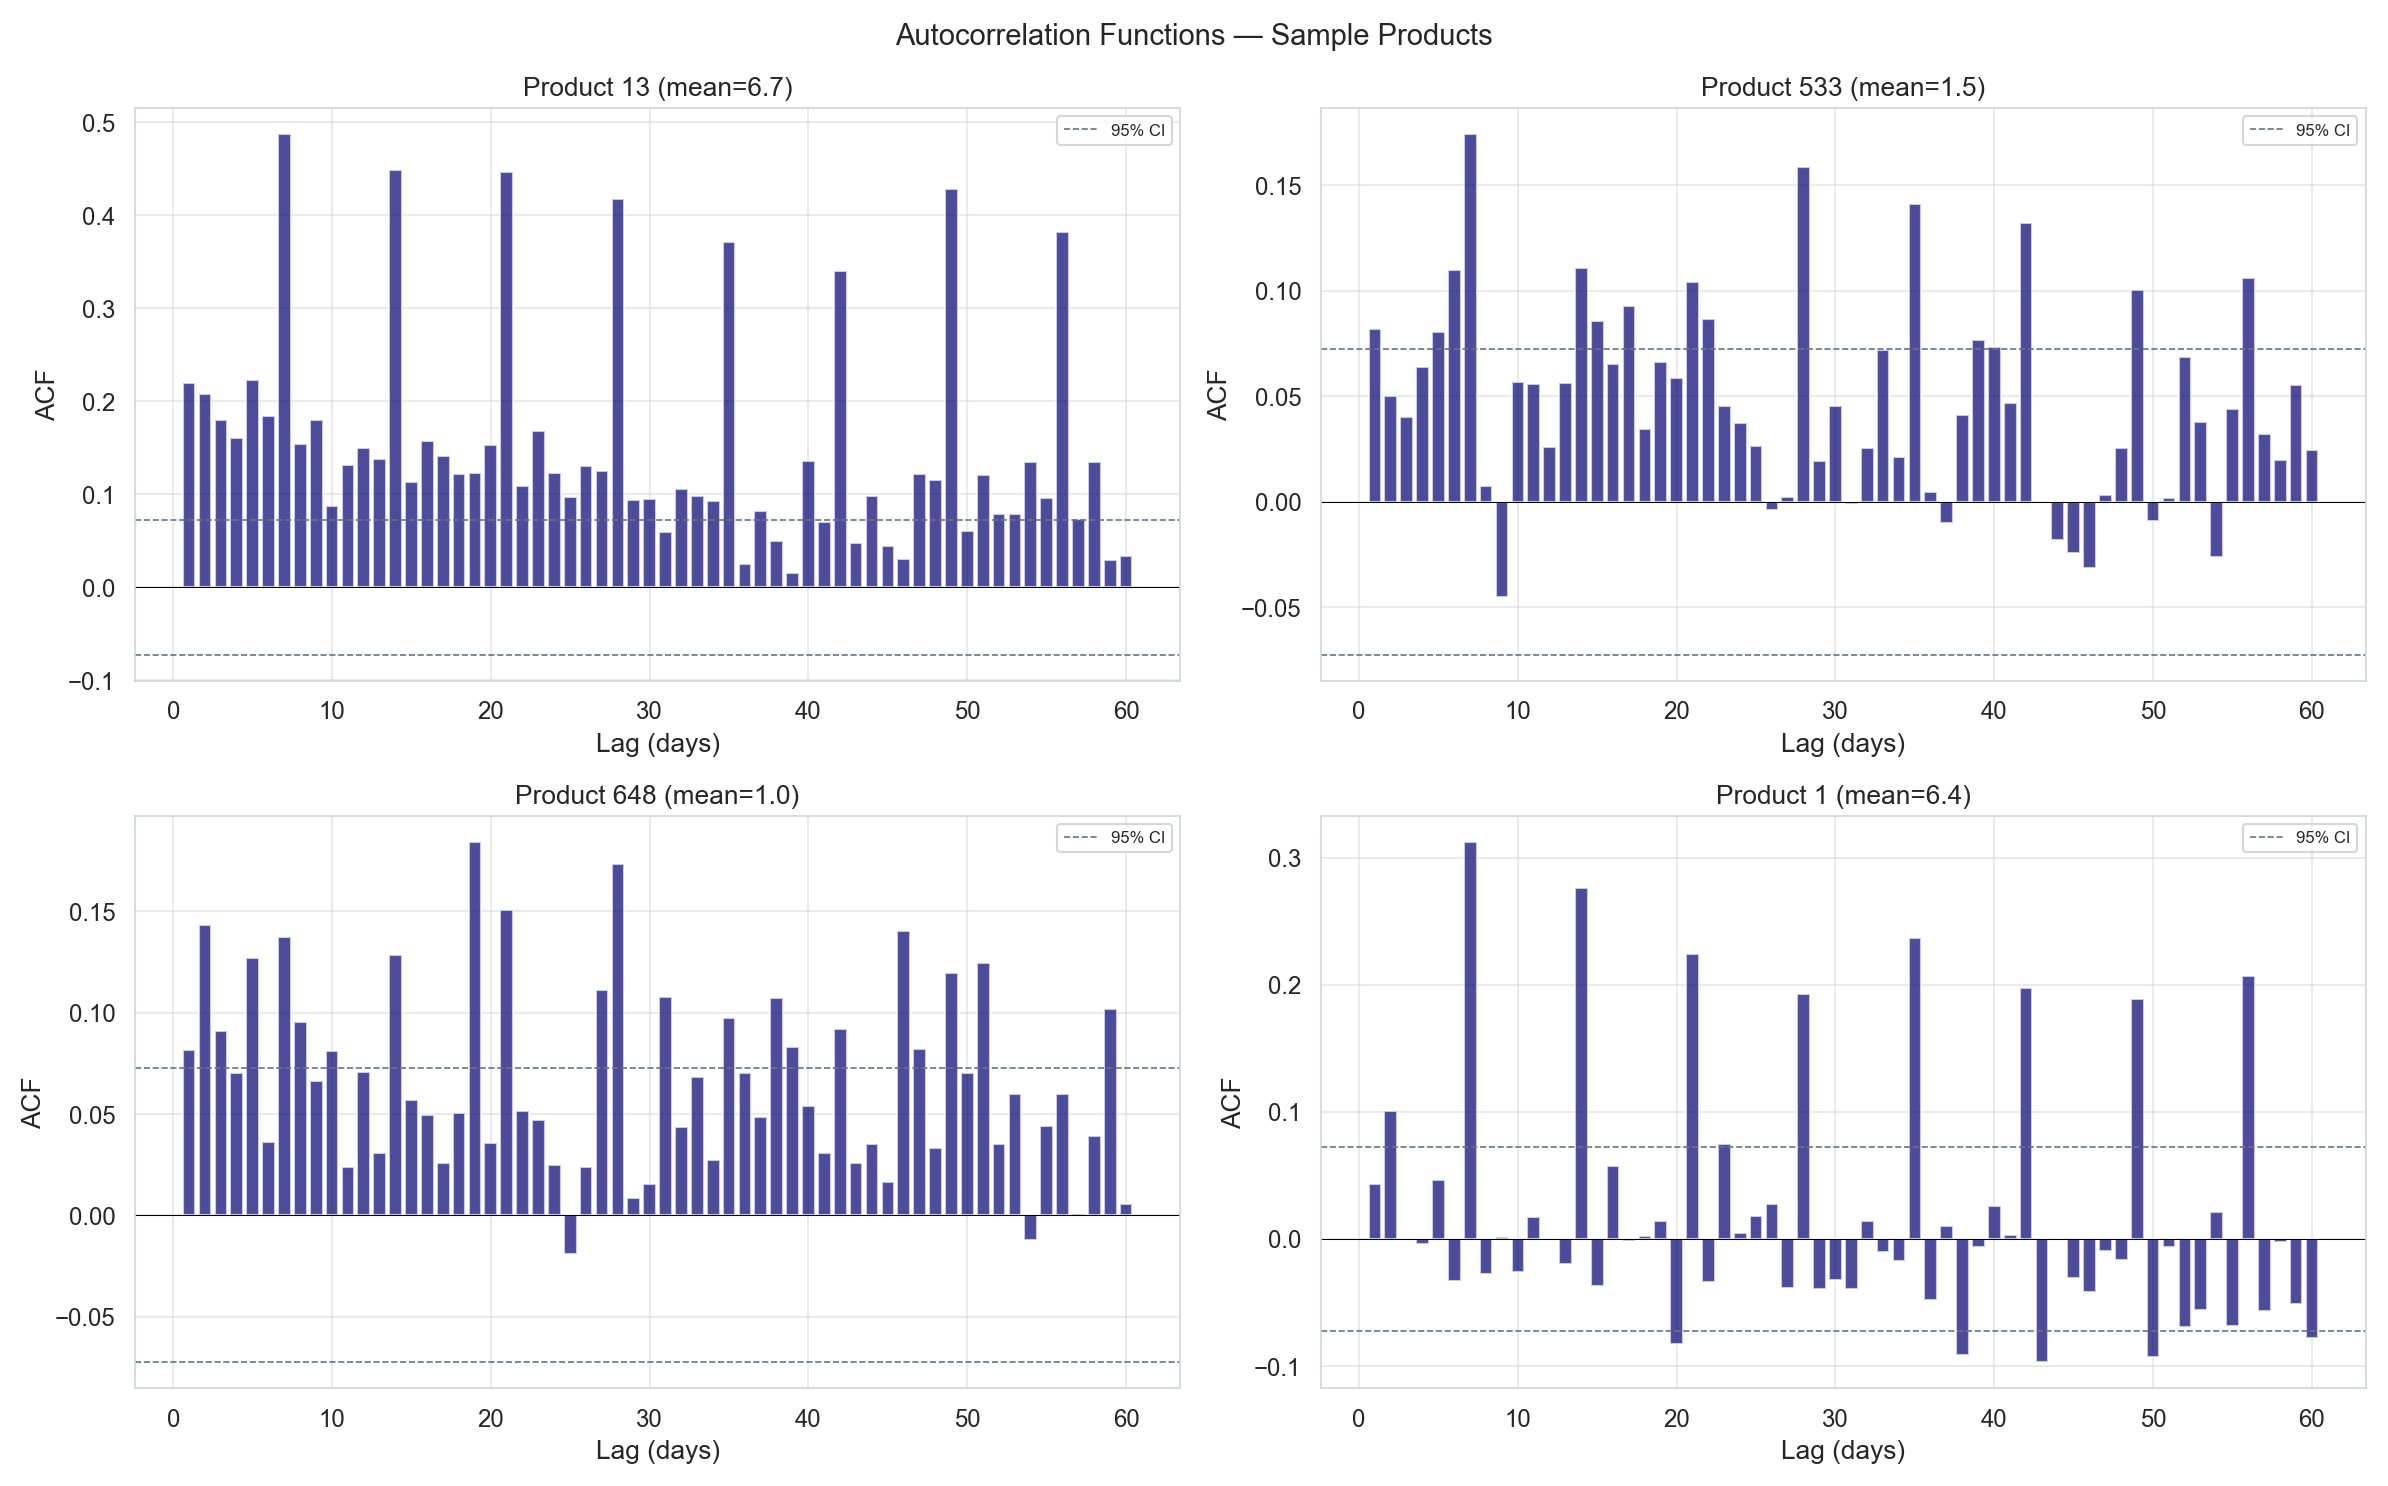
\includegraphics[width=0.85\textwidth]{figures/08_autocorrelation_sample.png}
\caption{Autocorrelation function (ACF) for a sample of products, showing significant positive autocorrelation at weekly intervals.}
\label{fig:autocorrelation}
\end{figure}

\subsection{Data Quality Analysis}

The data quality assessment identified the following issues:

\textbf{Missing values.} No explicit missing values were found in any of the four source tables. However, implicit gaps exist where lag features cannot be computed for the earliest dates in each product's history (addressed during feature engineering).

\textbf{Negative values.} No negative sales or stock values were present in this dataset.

\textbf{Stock breaks.} A stock break is defined as a day where both sales and stock are zero, potentially indicating that demand existed but could not be fulfilled due to inventory unavailability. Approximately 3.9\% of observations met this criterion. These were treated during data cleaning by imputing the product's historical mean sales for the corresponding weekday.

\textbf{Outliers.} Outlier detection was performed using a threshold of 1.75 times the interquartile range (IQR) per product. This identified approximately 11,400 observations (1.75\% of the dataset) as outliers, which were capped at the upper threshold value. The IQR-based approach was preferred over a fixed standard deviation threshold to account for the varying demand scales across products.


\section{Data Preparation}

\subsection{Data Cleaning}

The data cleaning process addressed the two quality issues identified during exploration:

\begin{enumerate}
    \item \textbf{Stock break imputation:} For observations where both \texttt{udsVenta} and \texttt{udsStock} were zero, the sales value was replaced with the mean sales for that product on the same weekday, computed over the preceding 30 days. This approach assumes that zero sales on a day with zero stock reflects a supply-side constraint rather than genuine zero demand, and uses a localised historical average to provide a reasonable demand estimate.

    \item \textbf{Outlier capping:} Values exceeding 1.75 $\times$ IQR above the 75th percentile for each product were capped at the threshold value. This preserves the general distribution shape while limiting the influence of extreme observations on model training. A total of 11,400 values (1.75\% of the dataset) were capped.
\end{enumerate}

After cleaning, the dataset retained its original 654,588 rows with no records removed, ensuring that the temporal continuity required for lag feature computation was preserved.

\subsection{Data Transformation}

The date column (\texttt{fecha}) was parsed into a \texttt{datetime} type, and the dataset was sorted by product and date to ensure correct temporal ordering for all subsequent operations. The promotional periods from the source data were transformed from date-range format into a daily binary indicator (\texttt{en\_promo}), assigned at the product-date level.

No logarithmic or power transformations were applied to the target variable. While such transformations can stabilise variance in skewed distributions, the tree-based models used in this work (Random Forest, XGBoost, LightGBM) are inherently robust to non-normal distributions and do not require target transformation for effective learning.

\subsection{Data Scaling}

Feature scaling (standardisation or normalisation) was not applied for the tree-based models, as decision tree ensembles are invariant to monotonic transformations of input features. The split-based learning mechanism of these algorithms operates on feature rankings rather than absolute values, making scaling unnecessary.

For the LSTM model, min-max normalisation was applied to all input features to facilitate gradient-based optimisation. Each feature was scaled to the $[0, 1]$ range using the training set statistics, and the same transformation was applied to the validation and test sets to prevent information leakage. Predictions were inverse-transformed back to the original scale before computing evaluation metrics.

\section{Feature Engineering}

Feature engineering is a central component of this work. A comprehensive set of 36 engineered features was designed to capture temporal dependencies, demand dynamics, and promotional effects. The features are organised into five categories, summarised in Table~\ref{tab:features}.

\begin{table}[H]
\centering
\small
\caption{Engineered features by category.}
\label{tab:features}
\begin{tabular}{|l|p{7cm}|r|}
\hline
\textbf{Category} & \textbf{Features} & \textbf{Count} \\
\hline
Original variables & udsStock, bolOpen, bolHoliday, en\_promo & 4 \\
\hline
Calendar features & year, month, day\_of\_week, week\_of\_year, week\_of\_month, is\_weekend, is\_month\_start, is\_month\_end & 8 \\
\hline
Lag features & lag\_1, lag\_7, lag\_14, lag\_28 & 4 \\
\hline
Rolling statistics & roll\_mean/std/min/max at 7, 14, and 28-day windows; ewma\_7, ewma\_28 & 14 \\
\hline
Promotional features & days\_since\_promo\_end, post\_promo\_7d, promo\_x\_lag7 & 3 \\
\hline
Product-level statistics & prod\_mean\_sales, prod\_std\_sales, prod\_median\_sales & 3 \\
\hline
\multicolumn{2}{|r|}{\textbf{Total}} & \textbf{36} \\
\hline
\end{tabular}
\end{table}

\textbf{Lag features} capture the autoregressive structure identified during exploration. The lag-7 feature (same weekday, previous week) serves dual purpose: it is used directly as the naive baseline forecast and as an input feature for the machine learning models. Lags at 1, 14, and 28 days capture short-term momentum, biweekly patterns, and monthly cycles respectively.

\textbf{Rolling statistics} provide smoothed representations of recent demand behaviour. For each window size (7, 14, and 28 days), the mean, standard deviation, minimum, and maximum of past sales are computed. Additionally, exponentially weighted moving averages (EWMA) with spans of 7 and 28 days provide adaptive smoothing that gives greater weight to more recent observations.

\textbf{Promotional features} go beyond the binary indicator to capture the temporal dynamics of promotions. The \texttt{days\_since\_promo\_end} feature tracks the recency of the last promotional period, \texttt{post\_promo\_7d} flags the week immediately following a promotion (to capture post-promotional demand depression), and \texttt{promo\_x\_lag7} is an interaction term between the promotional flag and the lag-7 sales value.

All lag and rolling features were computed strictly using past data to prevent information leakage. Observations where lag features could not be computed (the first 28 days of each product's history) were dropped, reducing the dataset from 654,588 to 629,370 rows. The final feature matrix was saved in Parquet format for use in the modelling phase.

\begin{figure}[H]
\centering
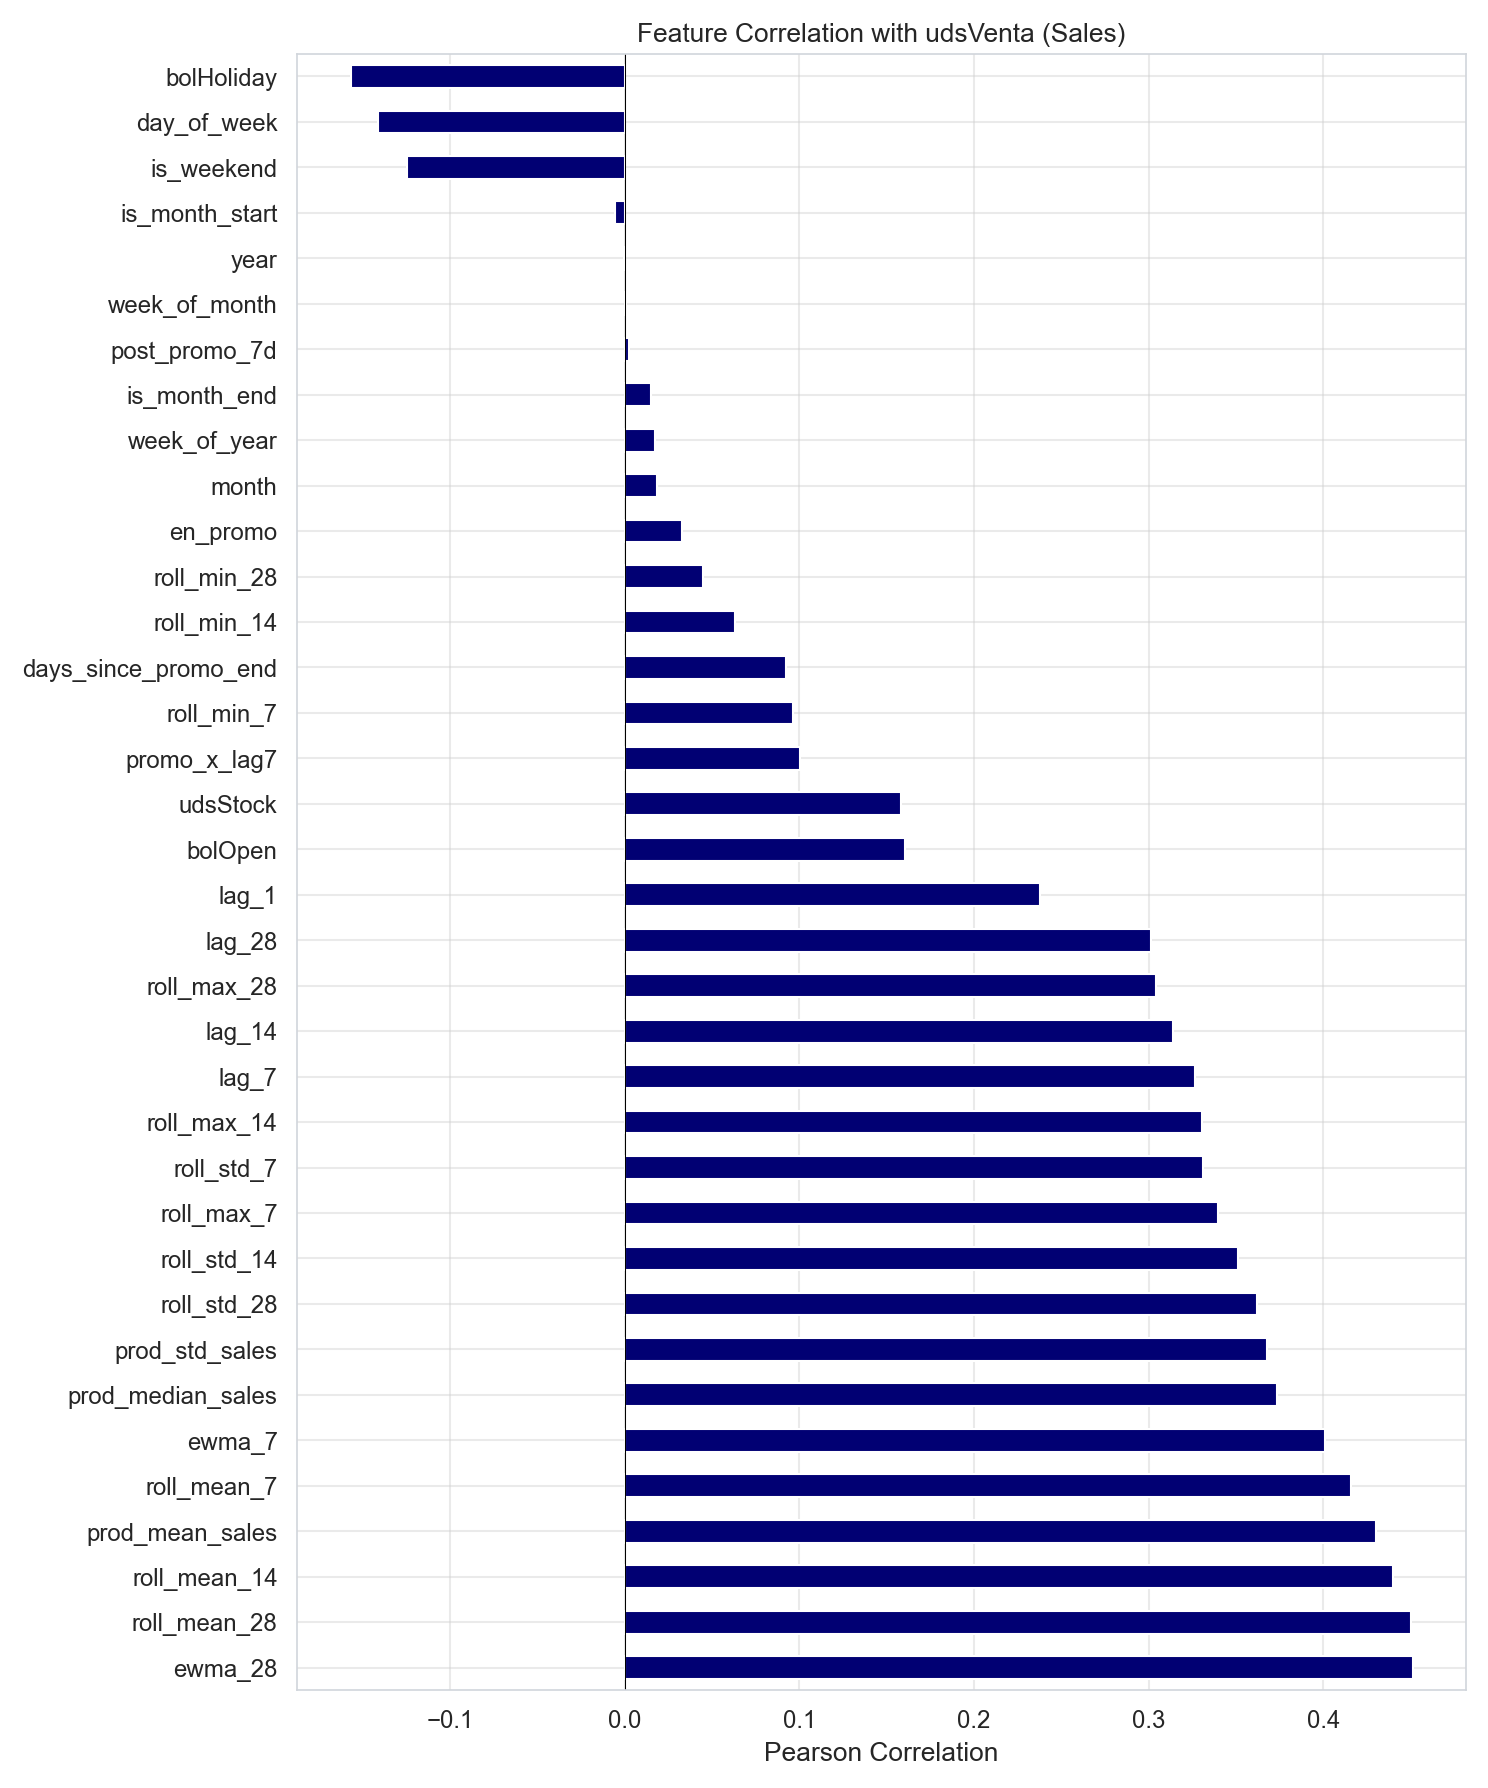
\includegraphics[width=0.95\textwidth]{figures/10_feature_correlations.png}
\caption{Correlation matrix of the engineered features. Strong correlations are visible among rolling statistics at different window sizes, confirming the presence of redundant but complementary temporal signals.}
\label{fig:feature_correlations}
\end{figure}


\section{Modelling}

\subsection{Model Selection}

Four forecasting approaches were implemented, spanning a naive baseline and three gradient boosting / ensemble methods:

\begin{enumerate}
    \item \textbf{Naive baseline (lag-7):} The simplest possible forecast, predicting that demand on any given day equals the demand observed on the same weekday of the previous week. This baseline exploits the strong weekly autocorrelation identified during exploration and provides a meaningful benchmark against which machine learning models must demonstrate improvement.

    \item \textbf{ARIMA (Seasonal):} A classical time series approach fitted per product using the \texttt{auto\_arima} implementation from the \texttt{pmdarima} library. Each product's demand series was modelled with seasonal ARIMA (SARIMA) with weekly periodicity ($m=7$), automatically selecting the optimal $(p,d,q)(P,D,Q)_7$ orders via stepwise search. ARIMA serves as the classical statistical baseline, representing the best that traditional time series methods can achieve without engineered features.

    \item \textbf{Random Forest:} An ensemble of decision trees trained on bootstrap samples with random feature subsets \citep{hyndman2021forecasting}. Random Forest provides robust predictions with built-in protection against overfitting through bagging and feature randomisation.

    \item \textbf{XGBoost:} A gradient boosting framework that builds trees sequentially, with each tree correcting the errors of its predecessors. XGBoost incorporates L1 and L2 regularisation, column subsampling, and efficient handling of sparse data, making it well-suited to the high proportion of zero-demand observations in this dataset.

    \item \textbf{LightGBM:} A gradient boosting implementation that uses histogram-based splitting and leaf-wise tree growth, offering faster training times than XGBoost while maintaining competitive accuracy. LightGBM was among the dominant algorithms in the M5 forecasting competition \citep{makridakis2021m5findings}.

    \item \textbf{LSTM (Long Short-Term Memory):} A recurrent neural network architecture designed to capture long-range temporal dependencies in sequential data \citep{hochreiter1997lstm}. Unlike tree-based methods, which rely on engineered lag features, LSTM processes input data as ordered sequences, with its internal gating mechanism allowing it to selectively retain or discard information from previous time steps. The model was implemented in PyTorch with a single LSTM layer (32 hidden units), trained on standardised features using 14-day input sequences.
\end{enumerate}

All tree-based models were trained on the full set of 33 input features (the 36 engineered features minus the 3 product-level statistics used only for reference). ARIMA was fitted per product on the raw sales series without engineered features, as is standard for classical time series methods. The LSTM model received the same 33 features as the tree models, but processed them as ordered sequences rather than independent observations. All predictions were clipped to a minimum of zero to prevent negative forecast values.

\subsection{Definition of Accuracy Indicators}

Four complementary metrics were used to evaluate forecast performance, as introduced in Chapter~2:

\begin{itemize}
    \item \textbf{MAE} (Mean Absolute Error): average absolute deviation between forecast and actual demand, in the same units as the target variable.
    \item \textbf{RMSE} (Root Mean Squared Error): penalises larger errors more heavily than MAE, providing a measure sensitive to occasional large deviations.
    \item \textbf{MAPE} (Mean Absolute Percentage Error): expresses errors as a percentage of actual demand, computed only for observations where actual demand is greater than zero to avoid division by zero.
    \item \textbf{$\sigma_e$} (forecast error standard deviation): the standard deviation of the residuals ($D_t - F_t$), which directly enters the safety stock calculation (Equation~\ref{eq:safety_stock}) and thus provides the link between forecast accuracy and inventory cost.
\end{itemize}

\subsection{Definition of Training and Validation Periods}

A rolling forecast origin validation strategy was adopted to provide a realistic assessment of out-of-sample performance by simulating the sequential nature of real forecasting decisions \citep{makridakis2021m5findings}.

Three validation folds were defined, each with a 30-day test window, working backwards from the most recent date in the dataset:

\begin{table}[H]
\centering
\small
\caption{Rolling forecast origin validation folds.}
\label{tab:folds}
\begin{tabular}{|c|c|c|c|}
\hline
\textbf{Fold} & \textbf{Training period end} & \textbf{Test period} & \textbf{Test days} \\
\hline
1 & 2024-09-06 & 2024-09-07 -- 2024-10-06 & 30 \\
2 & 2024-10-06 & 2024-10-07 -- 2024-11-05 & 30 \\
3 & 2024-10-06 & 2024-10-07 -- 2024-11-05 & 30 \\
\hline
\end{tabular}
\end{table}

For each fold, the training set includes all data up to the fold's cutoff date (expanding window), and the model is evaluated on the subsequent 30-day period. Final reported metrics are averaged across all three folds.

\subsection{Hyperparameter Tuning}

Hyperparameters for all three machine learning models were optimised using Optuna \citep{makridakis2021m5findings}, a Bayesian optimisation framework that efficiently explores the parameter space using a Tree-structured Parzen Estimator (TPE) sampler.

To balance computational cost with tuning quality, the optimisation was conducted on a representative subset of 50 randomly sampled products using the first validation fold. Each model was allocated 30 Optuna trials, with RMSE on the validation set as the objective function. The optimised hyperparameters were then applied to the full dataset across all validation folds.

Table~\ref{tab:tuned_params} presents the key tuned hyperparameters for each model:

\begin{table}[H]
\centering
\small
\caption{Optimised hyperparameters via Optuna (30 trials per model).}
\label{tab:tuned_params}
\begin{tabular}{|l|l|r|}
\hline
\textbf{Model} & \textbf{Parameter} & \textbf{Value} \\
\hline
\multirow{5}{*}{LightGBM} & n\_estimators & 300 \\
 & learning\_rate & 0.011 \\
 & num\_leaves & 75 \\
 & max\_depth & 4 \\
 & min\_child\_samples & 25 \\
\hline
\multirow{5}{*}{XGBoost} & n\_estimators & 350 \\
 & learning\_rate & 0.019 \\
 & max\_depth & 3 \\
 & min\_child\_weight & 10 \\
 & subsample & 0.90 \\
\hline
\multirow{4}{*}{Random Forest} & n\_estimators & 100 \\
 & max\_depth & 5 \\
 & min\_samples\_leaf & 16 \\
 & max\_features & 0.30 \\
\hline
\end{tabular}
\end{table}

The relatively shallow tree depths (3--5) and conservative learning rates (0.011--0.019) selected by the optimiser suggest that the models benefit from regularisation, which is consistent with the high proportion of zero-demand observations in the dataset.


\section{Evaluation}

\subsection{Accuracy Results Obtained}

Table~\ref{tab:results_summary} presents the average performance of each model across the three validation folds:

\begin{table}[H]
\centering
\small
\caption{Average forecast accuracy across three rolling validation folds.}
\label{tab:results_summary}
\begin{tabular}{|l|r|r|r|r|}
\hline
\textbf{Model} & \textbf{MAE} & \textbf{RMSE} & \textbf{MAPE (\%)} & \textbf{$\sigma_e$} \\
\hline
XGBoost & 1.366 & 2.155 & 52.2 & 2.154 \\
LightGBM & 1.373 & 2.158 & 51.7 & 2.158 \\
Random Forest & 1.394 & 2.176 & 51.6 & 2.176 \\
ARIMA$^\dagger$ & 1.443 & 2.220 & 59.8 & 2.219 \\
LSTM & 1.522 & 2.235 & 49.8 & 2.223 \\
Naive (lag-7) & 1.661 & 3.091 & 86.0 & 3.091 \\
\hline
\end{tabular}
\begin{flushleft}
\footnotesize{$^\dagger$ ARIMA evaluated on 50 sampled products due to per-product fitting cost.}
\end{flushleft}
\end{table}

All three tree-based machine learning models substantially outperform both the naive baseline and the classical/deep learning alternatives. XGBoost achieves the lowest RMSE (2.155), followed closely by LightGBM (2.158) and Random Forest (2.176). The RMSE improvement over the naive baseline ranges from 27.9\% (LSTM) to 30.3\% (XGBoost).

\begin{figure}[H]
\centering
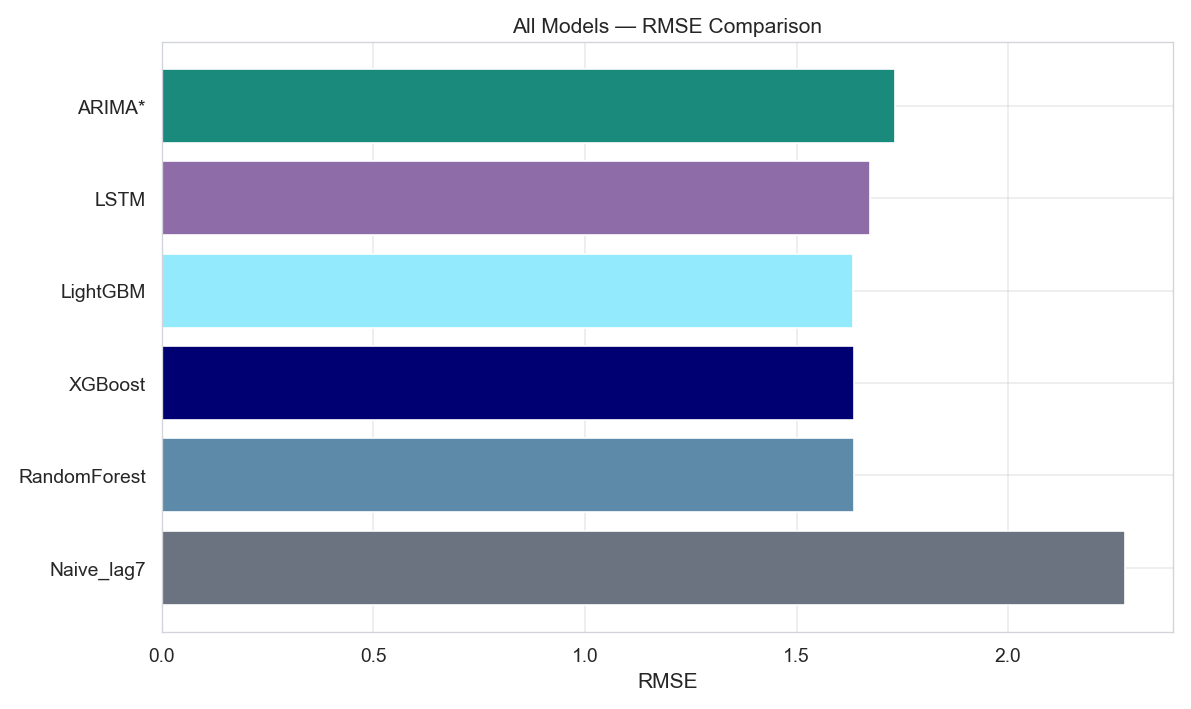
\includegraphics[width=0.85\textwidth]{figures/24_all_models_comparison.png}
\caption{Comparison of forecast accuracy (RMSE) across all six models. The three tree-based models form a tight cluster, substantially outperforming both classical and deep learning alternatives.}
\label{fig:all_models_comparison}
\end{figure}

ARIMA and LSTM occupy an intermediate position: both significantly outperform the naive baseline (RMSE reductions of 28.2\% and 27.7\% respectively) but fall short of the tree-based models. This result is consistent with the findings of the M5 forecasting competition \citep{makridakis2021m5findings}, where gradient boosting algorithms consistently outperformed both classical statistical methods and standalone deep learning approaches. The LSTM's slightly lower MAPE (49.8\%) but higher RMSE suggests it handles the zero-heavy distribution differently from tree models, producing fewer large percentage errors but occasionally larger absolute deviations.

\subsection{Comparison of Results Across Models}

\textbf{Promotional vs. non-promotional performance.} Table~\ref{tab:promo_results} compares model performance across demand segments:

\begin{table}[H]
\centering
\small
\caption{Model performance by demand segment (last validation fold).}
\label{tab:promo_results}
\begin{tabular}{|l|l|r|r|r|r|}
\hline
\textbf{Segment} & \textbf{Model} & \textbf{MAE} & \textbf{RMSE} & \textbf{MAPE (\%)} & \textbf{$\sigma_e$} \\
\hline
\multirow{4}{*}{Non-Promo} & XGBoost & 1.299 & 2.055 & 52.3 & 2.055 \\
 & LightGBM & 1.308 & 2.058 & 51.8 & 2.058 \\
 & Random Forest & 1.327 & 2.073 & 51.6 & 2.073 \\
 & Naive (lag-7) & 1.565 & 2.969 & 85.9 & 2.969 \\
\hline
\multirow{4}{*}{Promo} & XGBoost & 1.917 & 2.844 & 51.7 & 2.836 \\
 & LightGBM & 1.911 & 2.851 & 51.4 & 2.838 \\
 & Random Forest & 1.944 & 2.884 & 51.6 & 2.873 \\
 & Naive (lag-7) & 2.448 & 3.956 & 86.9 & 3.955 \\
\hline
\end{tabular}
\end{table}

Promotional demand is consistently harder to predict across all models, with RMSE values approximately 38\% higher than for non-promotional periods. However, the ML models maintain their advantage over the naive baseline in both segments, with RMSE improvements of approximately 28\% for non-promotional and 28\% for promotional demand.

\textbf{Per-product RMSE distribution.} Analysis at the individual product level reveals that LightGBM achieves a median per-product RMSE of 1.65, compared to 2.36 for the naive baseline. The improvement is not uniform: some products see RMSE reductions exceeding 15 units, while approximately 10 products show marginally worse performance with ML than with the naive approach. These products tend to have very low and stable demand where the simple lag-7 heuristic is already near-optimal.

\begin{figure}[H]
\centering
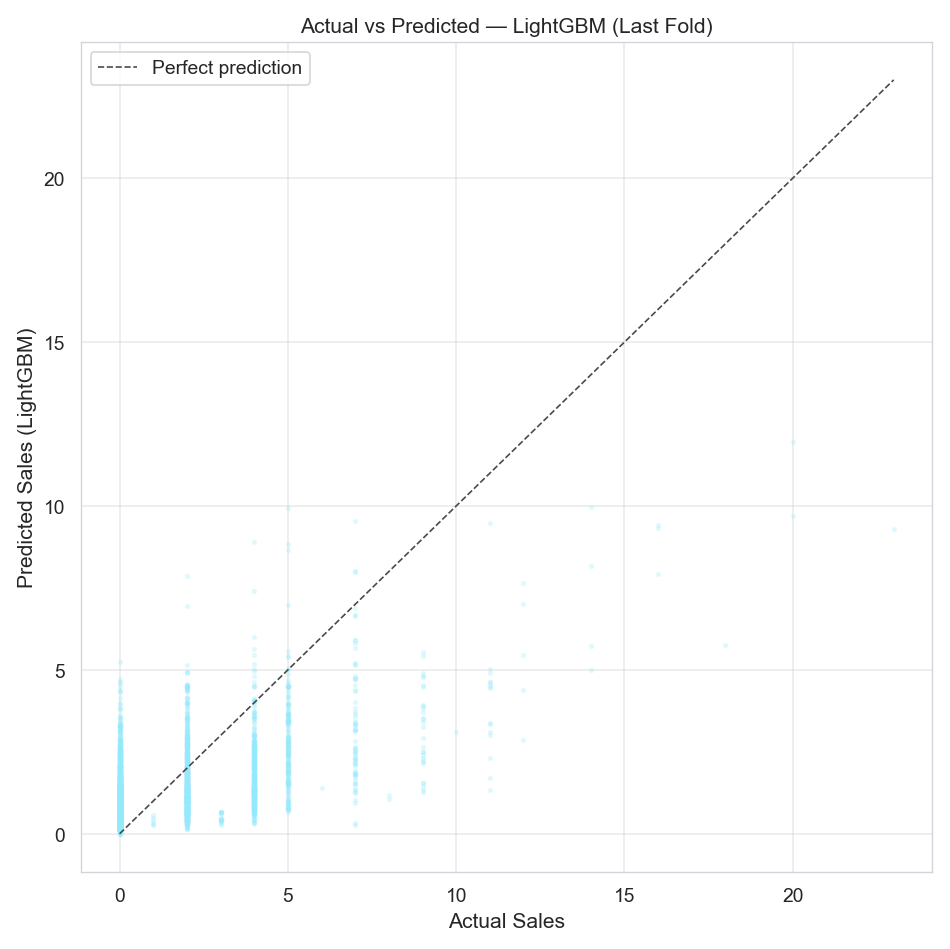
\includegraphics[width=0.85\textwidth]{figures/13_actual_vs_predicted_lgbm.png}
\caption{Actual vs.\ predicted sales for LightGBM on a sample of products. Points near the diagonal indicate accurate predictions; the cluster near the origin reflects the high proportion of zero-demand observations.}
\label{fig:actual_vs_predicted}
\end{figure}

\begin{figure}[H]
\centering
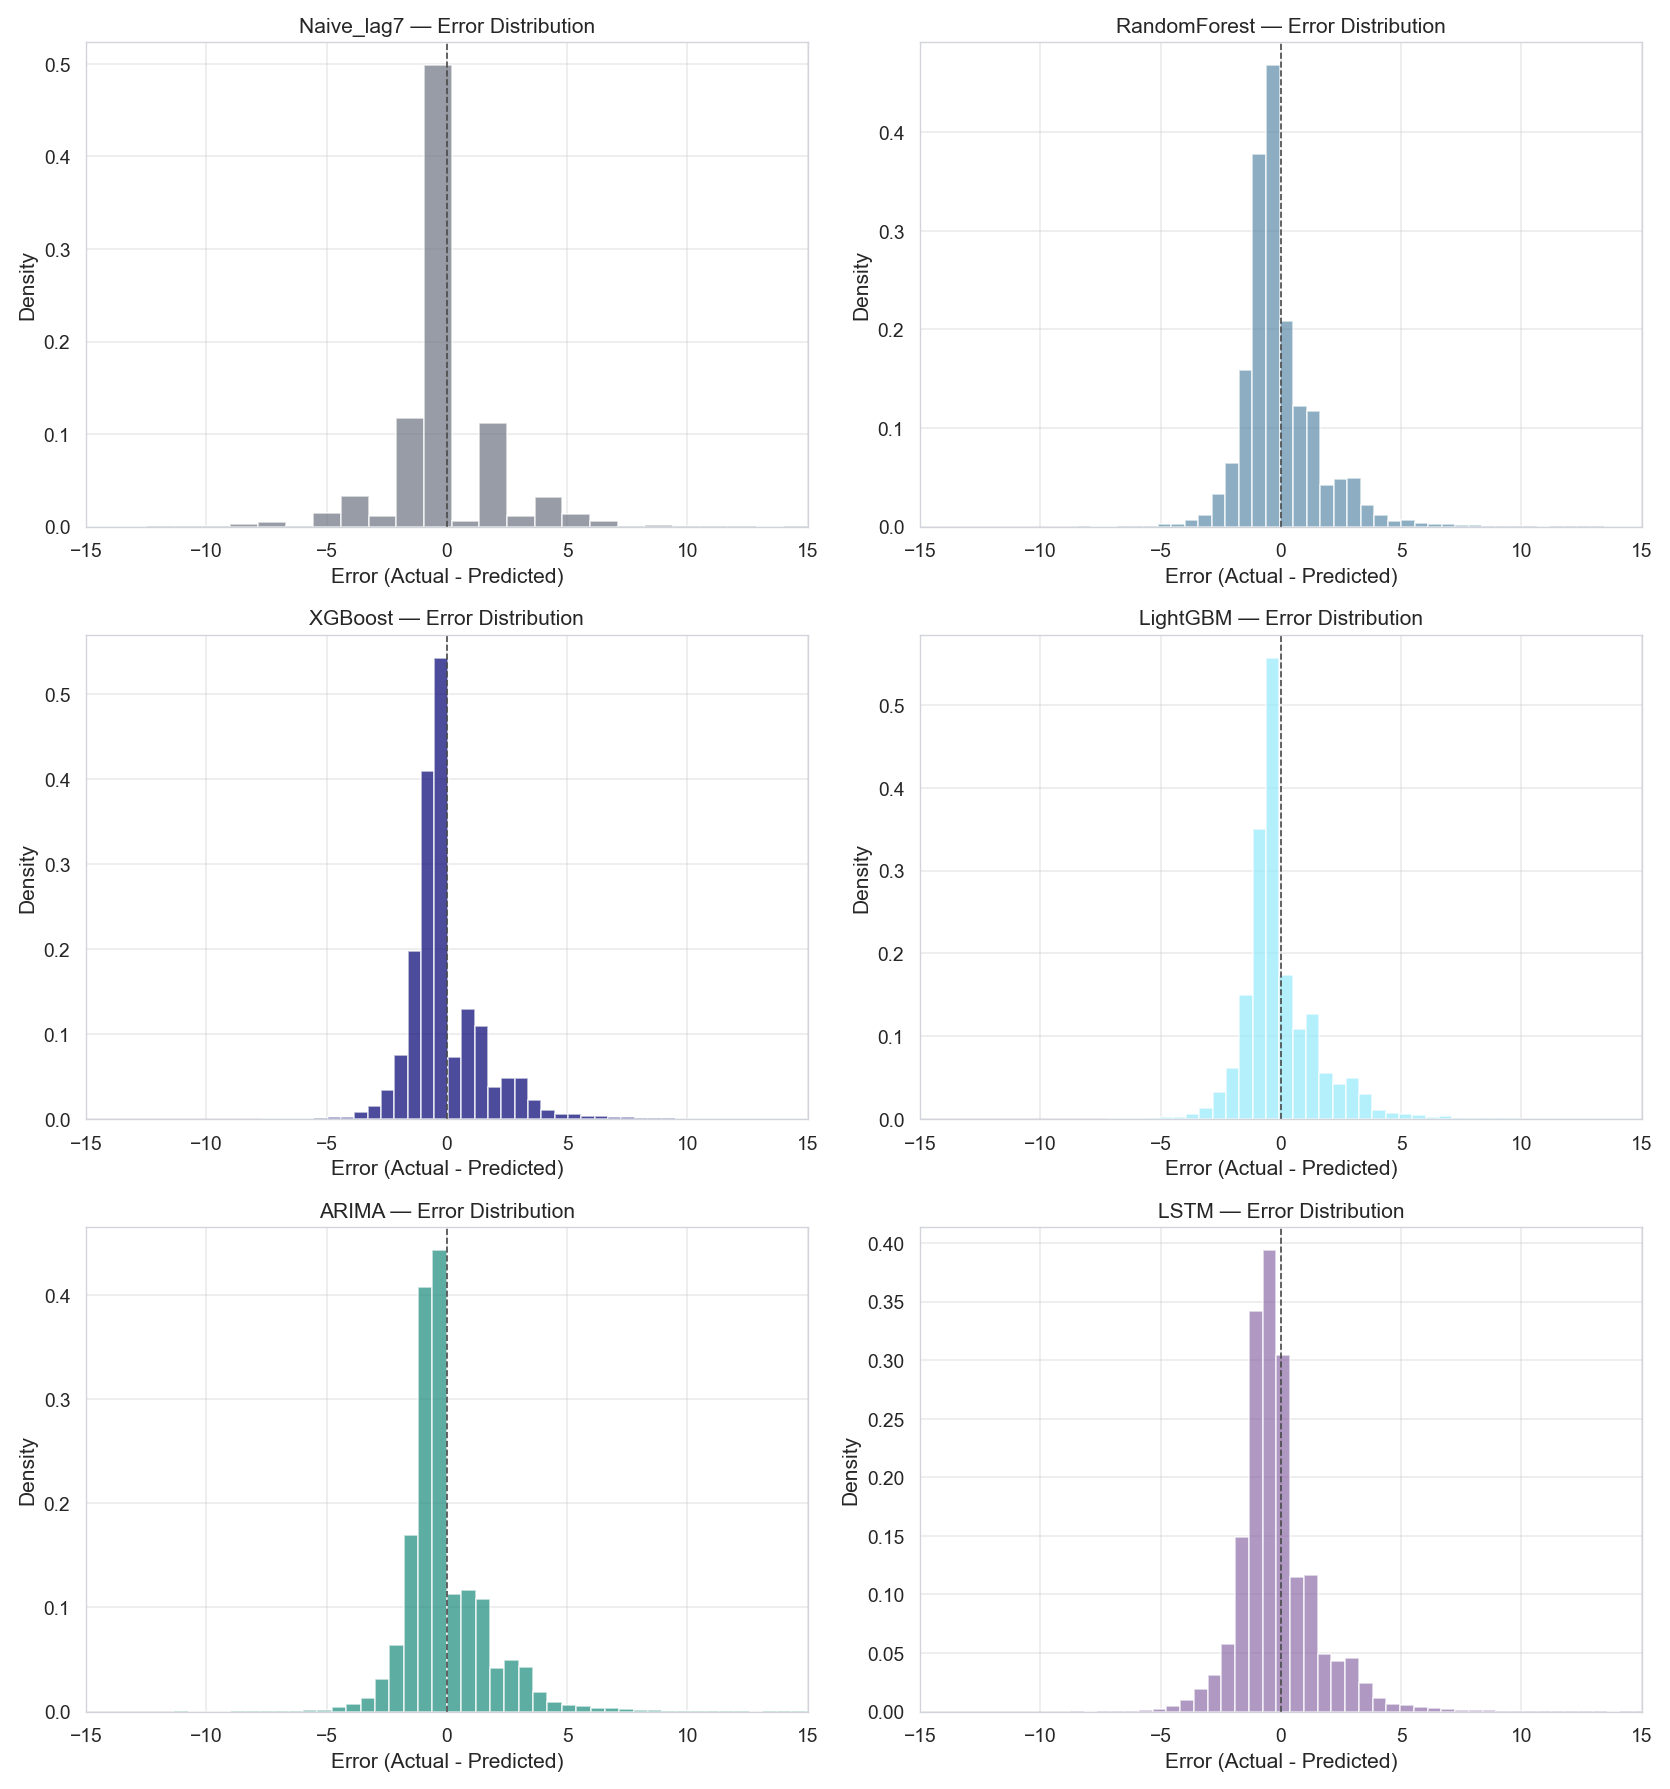
\includegraphics[width=0.85\textwidth]{figures/17_error_distributions.png}
\caption{Distribution of forecast errors by model. The ML models produce tighter, more symmetric error distributions compared to the naive baseline.}
\label{fig:error_distributions}
\end{figure}

\begin{figure}[H]
\centering
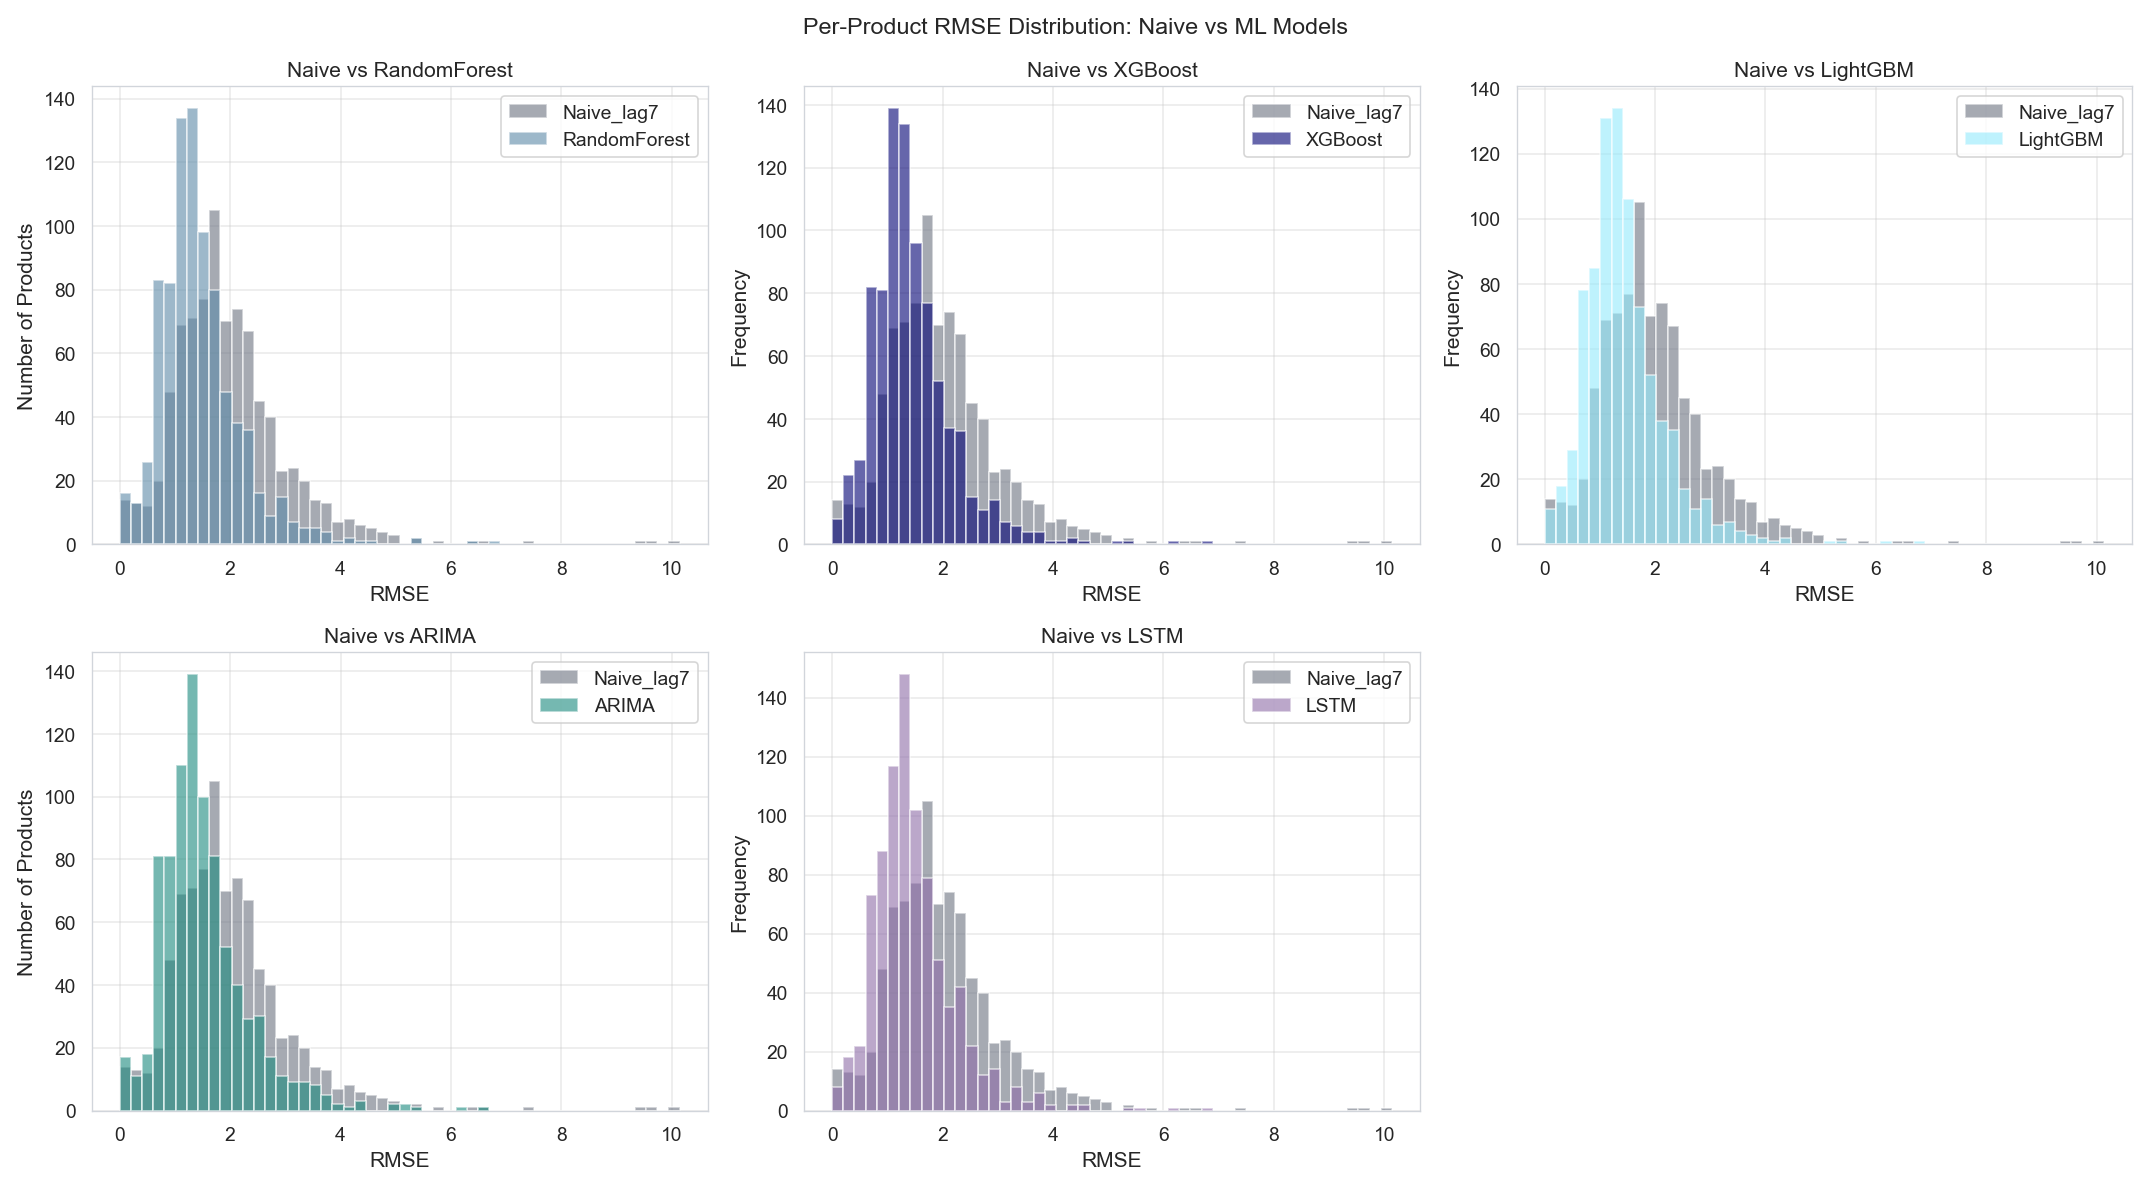
\includegraphics[width=0.85\textwidth]{figures/18_per_product_rmse_dist.png}
\caption{Distribution of per-product RMSE values. The ML models shift the distribution towards lower RMSE values compared to the naive baseline.}
\label{fig:per_product_rmse}
\end{figure}

\textbf{SHAP feature importance.} To understand the drivers of model predictions, SHAP (SHapley Additive exPlanations) analysis was performed on the LightGBM model. Table~\ref{tab:shap_top10} presents the ten most influential features:

\begin{table}[H]
\centering
\small
\caption{Top 10 features by mean absolute SHAP value (LightGBM).}
\label{tab:shap_top10}
\begin{tabular}{|r|l|r|}
\hline
\textbf{Rank} & \textbf{Feature} & \textbf{Mean $|$SHAP$|$} \\
\hline
1 & ewma\_28 & 0.524 \\
2 & bolHoliday & 0.295 \\
3 & roll\_mean\_28 & 0.150 \\
4 & day\_of\_week & 0.079 \\
5 & udsStock & 0.063 \\
6 & roll\_max\_28 & 0.046 \\
7 & lag\_28 & 0.025 \\
8 & bolOpen & 0.022 \\
9 & roll\_mean\_14 & 0.017 \\
10 & roll\_max\_14 & 0.016 \\
\hline
\end{tabular}
\end{table}

The 28-day EWMA emerges as the single most important predictor, followed by the holiday indicator and the 28-day rolling mean. This confirms that the model relies heavily on smoothed representations of recent demand history, with calendar effects providing secondary but significant predictive power. Notably, the longer-horizon features (28-day windows) dominate over shorter-horizon ones (7-day), suggesting that the model captures medium-term demand trends rather than relying solely on short-term momentum.

\begin{figure}[H]
\centering
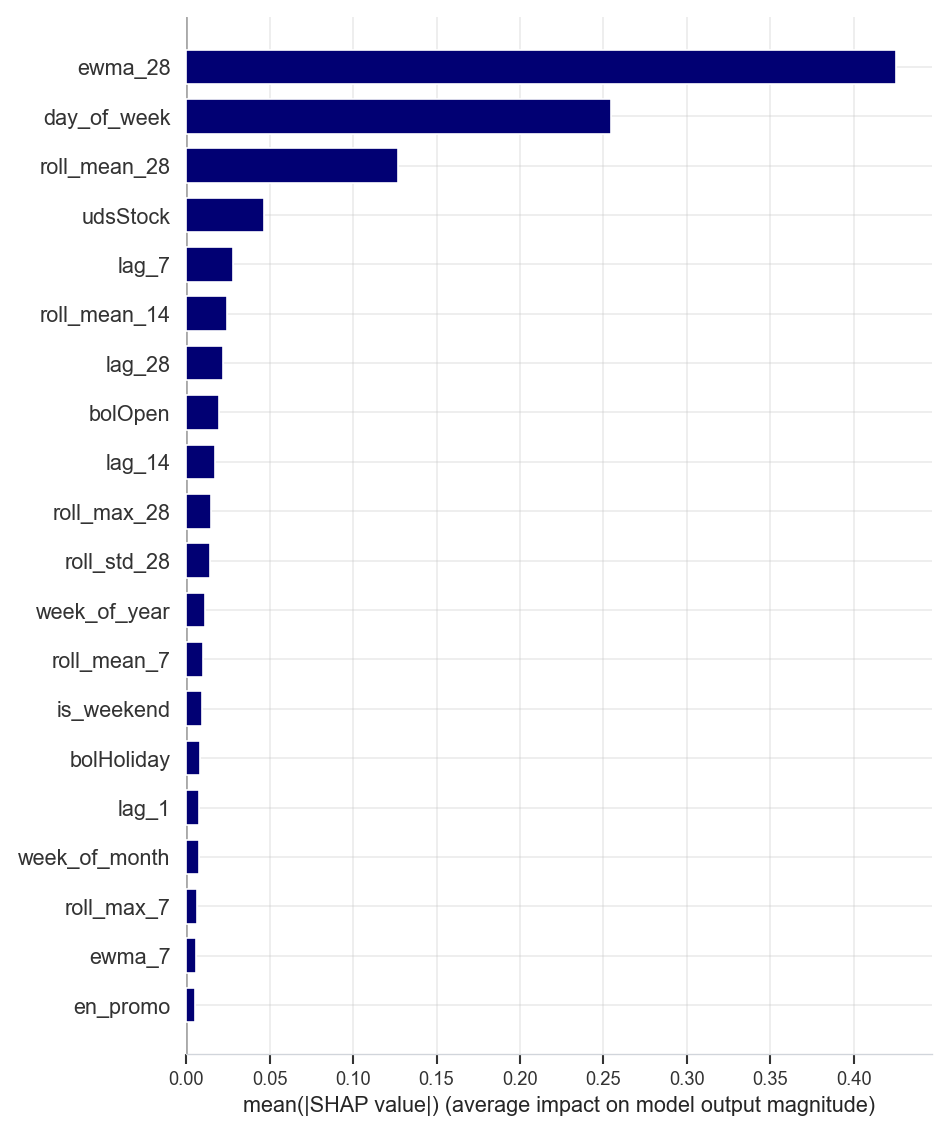
\includegraphics[width=0.85\textwidth]{figures/15_shap_bar.png}
\caption{SHAP feature importance (mean absolute SHAP values) for LightGBM. The 28-day EWMA dominates, followed by calendar and rolling statistics features.}
\label{fig:shap_bar}
\end{figure}

\begin{figure}[H]
\centering
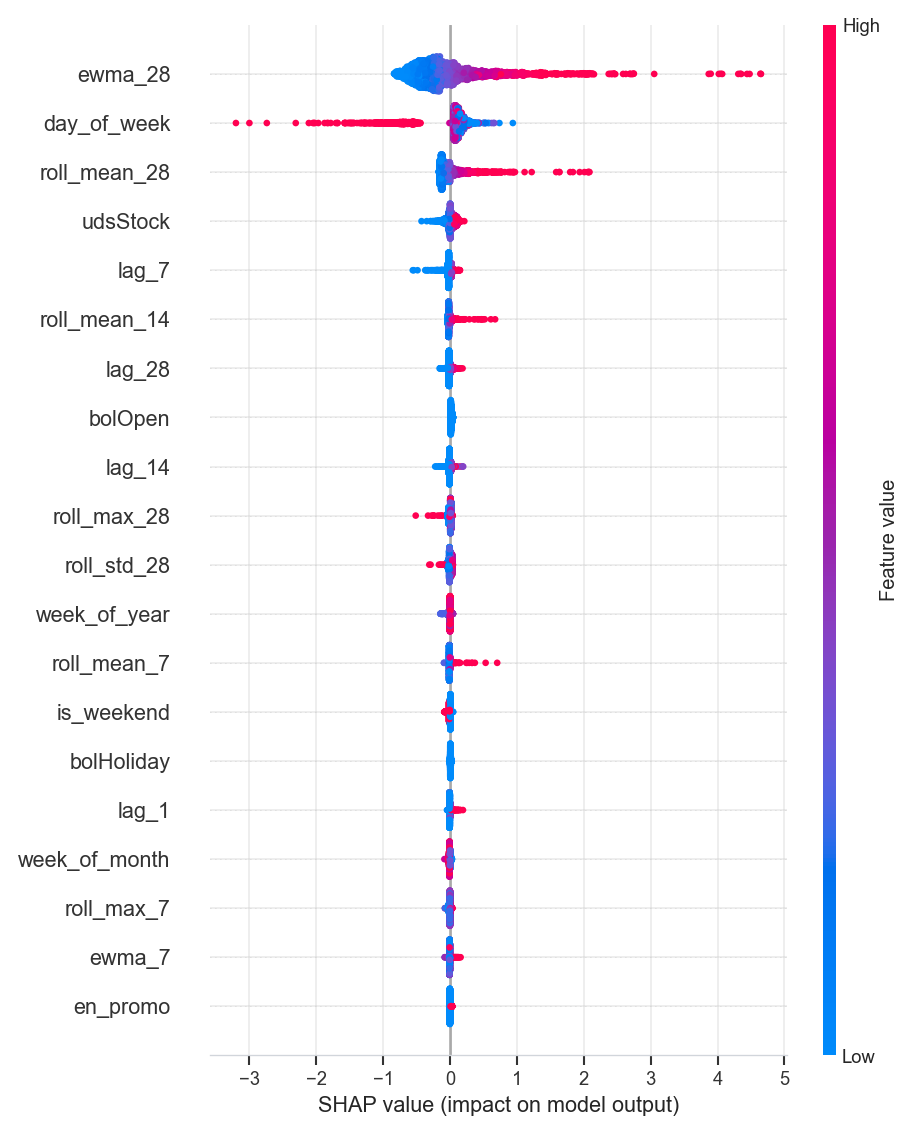
\includegraphics[width=0.85\textwidth]{figures/14_shap_summary.png}
\caption{SHAP summary plot showing the direction and magnitude of feature effects. Red indicates high feature values; blue indicates low values. High \texttt{ewma\_28} values push predictions upward, consistent with higher recent demand leading to higher forecasts.}
\label{fig:shap_summary}
\end{figure}

\subsection{Conclusions from Results}

The evaluation yields several key findings:

\begin{enumerate}
    \item The three tree-based machine learning models (XGBoost, LightGBM, Random Forest) achieve the best performance, with RMSE values within 1\% of each other. This suggests that the feature engineering, rather than the specific algorithm choice, is the primary driver of forecast quality among this model family.

    \item ARIMA and LSTM occupy an intermediate tier, both significantly outperforming the naive baseline (RMSE reductions of 28\% and 28\% respectively) but falling short of the tree-based models. ARIMA's per-product fitting captures local demand patterns effectively but cannot leverage cross-product information or engineered features. LSTM captures sequential dependencies but requires substantially more training data and computation to match tree-based performance.

    \item The improvement over the naive baseline is substantial across all ML approaches (28--30\% RMSE reduction), demonstrating the value of incorporating engineered features and systematic model training over simple heuristic forecasting.

    \item Promotional demand remains the most challenging segment, with RMSE approximately 38\% higher than non-promotional demand across all models. However, the ML models maintain their relative advantage over the baseline in both segments.

    \item SHAP analysis reveals that smoothed demand history (EWMA and rolling statistics) and calendar features are the most influential predictors, validating the feature engineering strategy adopted in this work.

    \item The forecast error standard deviation ($\sigma_e \approx 2.15$ for the best tree models, $\sigma_e \approx 2.22$ for ARIMA/LSTM, compared to $\sigma_e \approx 3.09$ for the naive baseline) translates directly into safety stock reductions, as quantified in the following section.
\end{enumerate}


\section{Impact of Algorithm Improvement}

\subsection{Impact on Processes}

The transition from a naive forecasting approach to machine learning models has implications beyond numerical accuracy improvements. From an operational perspective, the key process impacts are:

\textbf{Safety stock reduction.} Using the safety stock formulation from Equation~\ref{eq:safety_stock} with a 95\% service level ($z = 1.645$) and a protection period of 10 days (3 days lead time + 7 days review period), the total safety stock across all 894 products decreases from 11,953 units under the naive forecast to 8,276 units under LightGBM --- a reduction of 30.8\%. This means that the same service level can be maintained with significantly less inventory investment.

\textbf{Forecast error symmetry.} Analysis of error distributions shows that the ML models produce approximately symmetric errors centred near zero, whereas the naive baseline exhibits a slight positive bias (tendency to overforecast). Symmetric errors are preferable for inventory planning, as they indicate that the forecast is equally likely to overestimate or underestimate demand, allowing safety stock to function as intended.

\textbf{Sensitivity to service level.} Table~\ref{tab:sensitivity} presents the total safety stock requirements across different service levels:

\begin{table}[H]
\centering
\small
\caption{Total safety stock (units) by model and service level.}
\label{tab:sensitivity}
\begin{tabular}{|l|r|r|r|}
\hline
\textbf{Model} & \textbf{90\%} & \textbf{95\%} & \textbf{99\%} \\
\hline
LightGBM & 6,450 & 8,276 & 11,702 \\
XGBoost & 6,466 & 8,296 & 11,731 \\
Random Forest & 6,507 & 8,350 & 11,806 \\
Naive (lag-7) & 9,316 & 11,953 & 16,902 \\
\hline
\end{tabular}
\end{table}

The ML models consistently require approximately 30\% less safety stock than the naive baseline across all service levels, demonstrating that the improvement is robust and not dependent on a specific service level assumption.

\begin{figure}[H]
\centering
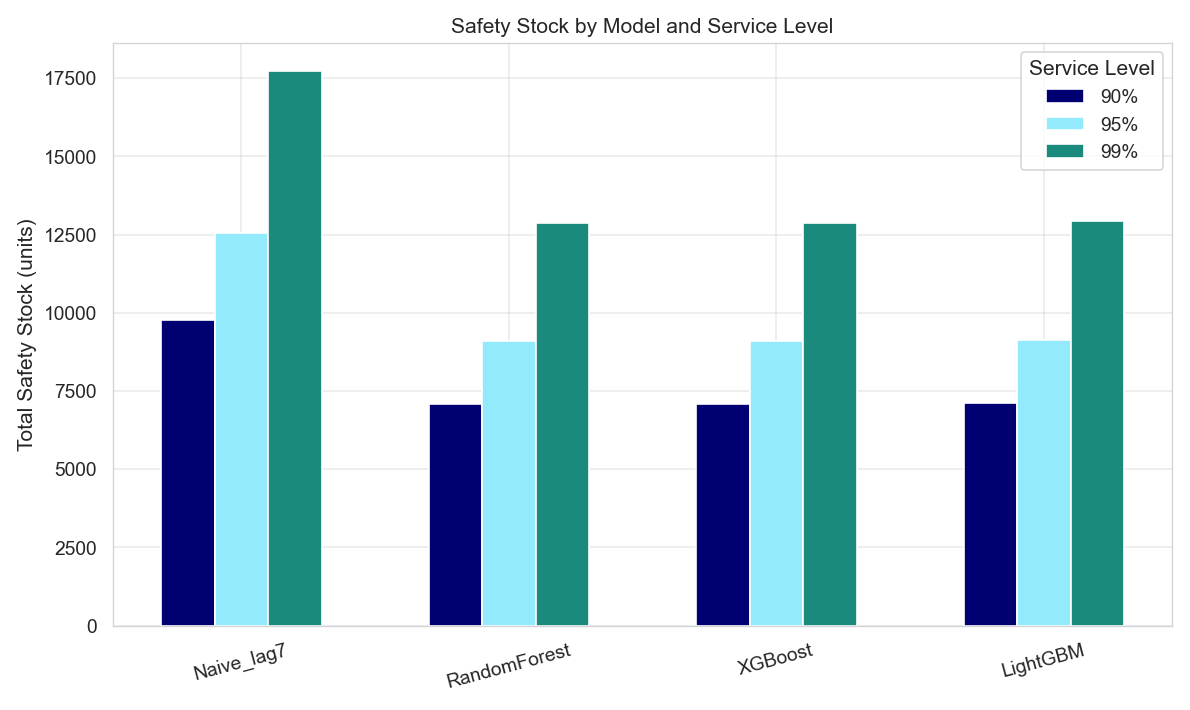
\includegraphics[width=0.85\textwidth]{figures/21_safety_stock_by_service_level.png}
\caption{Total safety stock requirements by model and service level. The ML models maintain a consistent ~30\% advantage over the naive baseline across all service levels.}
\label{fig:safety_stock_service_level}
\end{figure}

\subsection{Economic Impact}

The economic impact analysis combines two cost components: the newsvendor cost (direct cost of forecast errors) and the safety stock holding cost.

\textbf{Newsvendor cost analysis.} Following the total cost formulation from Equation~\ref{eq:total_cost}, the asymmetric costs of overforecasting and underforecasting were computed using cost parameters of $C_o = \text{\euro}0.10$ per unit per day (overage/holding) and $C_u = \text{\euro}0.50$ per unit per day (underage/lost sale), yielding a critical ratio of 0.83. These values reflect a typical retail/industrial setting where stockout costs substantially exceed holding costs.

Table~\ref{tab:newsvendor} presents the newsvendor cost results:

\begin{table}[H]
\centering
\small
\caption{Newsvendor cost analysis (30-day test period, annualised).}
\label{tab:newsvendor}
\begin{tabular}{|l|r|r|r|r|}
\hline
\textbf{Model} & \textbf{Overage (€)} & \textbf{Underage (€)} & \textbf{Total (€)} & \textbf{Annual est. (€)} \\
\hline
Naive (lag-7) & 2,227 & 11,138 & 13,365 & 162,603 \\
Random Forest & 1,830 & 9,538 & 11,367 & 138,304 \\
LightGBM & 1,786 & 9,489 & 11,275 & 137,182 \\
XGBoost & 1,785 & 9,392 & 11,176 & 135,979 \\
\hline
\end{tabular}
\end{table}

XGBoost achieves the lowest newsvendor cost, saving approximately \euro26,600 annually (16.4\%) compared to the naive baseline. Underage costs dominate in all models, consistent with the asymmetric cost structure where stockouts are five times more expensive than excess inventory.

\textbf{Combined cost analysis.} Table~\ref{tab:combined_cost} presents the total annual cost combining newsvendor costs with safety stock holding costs at the 95\% service level:

\begin{table}[H]
\centering
\small
\caption{Combined annual cost: newsvendor + safety stock holding (95\% service level).}
\label{tab:combined_cost}
\begin{tabular}{|l|r|r|r|}
\hline
\textbf{Model} & \textbf{Newsvendor (€/yr)} & \textbf{SS Holding (€/yr)} & \textbf{Total (€/yr)} \\
\hline
Naive (lag-7) & 162,603 & 436,294 & 598,896 \\
Random Forest & 138,304 & 304,763 & 443,067 \\
LightGBM & 137,182 & 302,083 & 439,265 \\
XGBoost & 135,979 & 302,816 & 438,796 \\
\hline
\end{tabular}
\end{table}

The ML models achieve total annual cost savings of approximately \euro160,000 (26.7\%) compared to the naive baseline. XGBoost and LightGBM perform nearly identically in economic terms, with XGBoost holding a marginal advantage of \euro469 annually.

\begin{figure}[H]
\centering
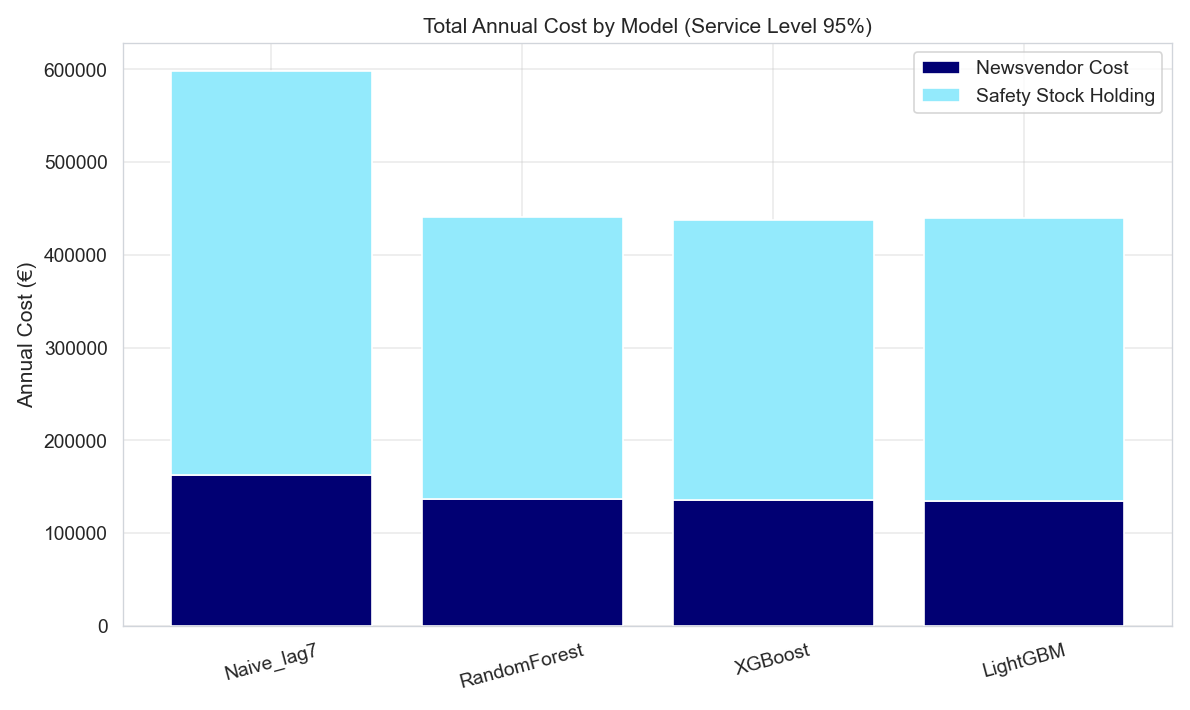
\includegraphics[width=0.85\textwidth]{figures/22_combined_annual_cost.png}
\caption{Combined annual inventory cost (newsvendor + safety stock holding) by model. The ML models reduce total costs by approximately 26.7\% compared to the naive baseline.}
\label{fig:combined_annual_cost}
\end{figure}

These results demonstrate that the forecast accuracy improvements documented in Section~3.6 translate into meaningful economic benefits. The 28\% reduction in RMSE corresponds to a 26.7\% reduction in total inventory-related costs, confirming the theoretical relationship between forecast error and inventory costs established in Chapter~2 (Equations~\ref{eq:ss_cost} and \ref{eq:total_cost}).

It is important to note that the cost parameters used in this analysis ($C_o$ and $C_u$) are illustrative values chosen to reflect typical industrial cost structures. The relative ranking of models and the percentage savings are robust to reasonable variations in these parameters, as the underlying driver is the reduction in forecast error rather than the specific cost assumptions. A sensitivity analysis across service levels (Table~\ref{tab:sensitivity}) confirms that the ML advantage is maintained regardless of the risk tolerance adopted by the organisation.
 in TFM_onamas.tex

This chapter presents the complete design and implementation of the demand forecasting system, following the CRISP-DM methodology introduced in Chapter~1. The work progresses from data acquisition and exploration through preprocessing, feature engineering, model development, evaluation, and finally the economic impact analysis that connects forecast accuracy to inventory cost savings.

\section{Data Origin}

\subsection{Data Acquisition}

The dataset used in this project was provided by the thesis supervisor and corresponds to real historical data from a company operating in the automotive sector. The data covers daily demand records for a portfolio of products, along with supplementary information on calendar events, promotional campaigns, and stock levels. All data was received in a single Microsoft Excel file (\texttt{Datos.xlsx}) containing four sheets, each representing a distinct dimension of the business context.

No personally identifiable information is present in the dataset, and all product references are anonymised using numerical identifiers, ensuring compliance with data privacy requirements as discussed in Section~\ref{s:etic}.

\subsection{Data Description}

The dataset comprises four tables, summarised in Table~\ref{tab:data_sheets}:

\begin{table}[H]
\centering
\small
\caption{Structure of the source dataset (\texttt{Datos.xlsx}).}
\label{tab:data_sheets}
\begin{tabular}{|l|l|r|p{5.5cm}|}
\hline
\textbf{Sheet} & \textbf{Key columns} & \textbf{Rows} & \textbf{Description} \\
\hline
Ventas (Sales) & producto, fecha, udsVenta & 654,588 & Daily unit sales per product \\
\hline
Calendario & fecha, bolOpen, bolHoliday & 732 & Calendar flags: business day and holiday indicators \\
\hline
Promociones & producto, fechaInicio, fechaFin & 1,894 & Promotional campaign periods per product \\
\hline
Stock & producto, fecha, udsStock & 654,588 & Daily stock levels per product \\
\hline
\end{tabular}
\end{table}

The sales sheet constitutes the core of the dataset, containing 654,588 daily observations across 894 unique products over a period of 732 days, spanning from November 2022 to November 2024. Each record represents the number of units sold for a specific product on a specific date.

The calendar sheet provides 732 daily records with two binary indicators: \texttt{bolOpen} (whether the business was open) and \texttt{bolHoliday} (whether the date was a public holiday). The promotions sheet contains 1,894 records defining promotional campaign windows through start and end dates for each product. The stock sheet mirrors the sales structure, recording the closing stock level for each product-date combination.

\subsection{Data Loading}

All four sheets were loaded into memory using the \texttt{pandas} library with the \texttt{openpyxl} engine. The sales and stock tables were merged on the shared keys \texttt{(producto, fecha)}, and the calendar information was joined on \texttt{fecha}. Promotional periods were transformed from date ranges into a binary indicator (\texttt{en\_promo}) at the product-date level, marking each observation as promotional or non-promotional based on whether the date fell within any active campaign for that product.

After merging, the resulting dataset contained 654,588 rows and served as the foundation for all subsequent analysis. The merged dataset was persisted in Apache Parquet format for efficient reloading in downstream scripts.


\section{Data Exploration}

\subsection{Data Summary}

An initial statistical summary of the target variable (\texttt{udsVenta}, units sold) revealed a highly skewed distribution. The mean daily sales per product were 1.42 units, with a median of zero and a standard deviation of 3.56. The maximum observed value was 99 units. This distribution reflects the nature of automotive parts demand, where the majority of product-day combinations register zero sales, punctuated by occasional larger orders.

Table~\ref{tab:sales_stats} presents the key descriptive statistics:

\begin{table}[H]
\centering
\small
\caption{Descriptive statistics of daily unit sales (\texttt{udsVenta}).}
\label{tab:sales_stats}
\begin{tabular}{|l|r|}
\hline
\textbf{Statistic} & \textbf{Value} \\
\hline
Count & 654,588 \\
Mean & 1.42 \\
Std. deviation & 3.56 \\
Median (50\%) & 0.00 \\
75th percentile & 1.00 \\
95th percentile & 7.00 \\
Maximum & 99 \\
Zero-sales proportion & 64.5\% \\
\hline
\end{tabular}
\end{table}

The high proportion of zero-sales observations (64.5\%) is a defining characteristic of this dataset and has important implications for model selection and evaluation, as discussed in subsequent sections.

\begin{figure}[H]
\centering
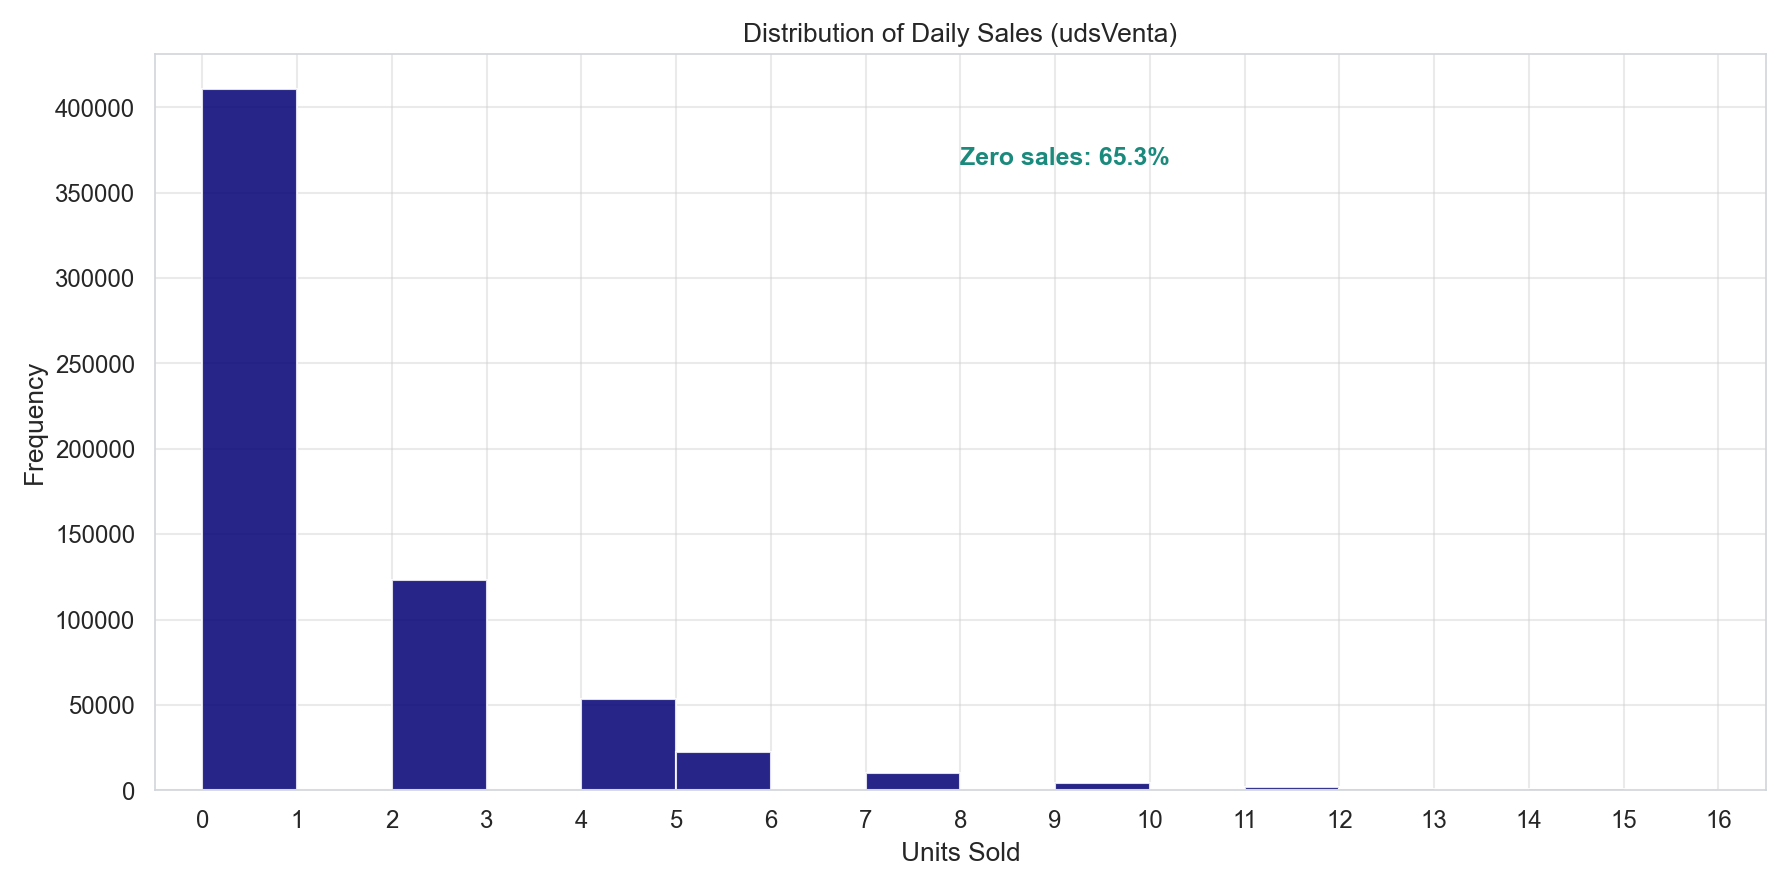
\includegraphics[width=0.85\textwidth]{figures/01_sales_distribution.png}
\caption{Distribution of daily unit sales (\texttt{udsVenta}). The histogram confirms the extreme right skew, with the majority of observations at zero.}
\label{fig:sales_distribution}
\end{figure}

\subsection{Statistical Analysis}

The exploratory analysis examined demand patterns across several dimensions:

\textbf{Day-of-week patterns.} Sales exhibit a clear weekly cycle, with the highest volumes on weekdays (Monday through Friday) and a sharp decline on Saturdays. Sunday sales are near zero, consistent with the business being closed on Sundays as indicated by the \texttt{bolOpen} calendar flag. This weekly seasonality motivates the inclusion of day-of-week features and the use of a lag-7 naive baseline (same weekday, previous week) as the primary benchmark.

\begin{figure}[H]
\centering
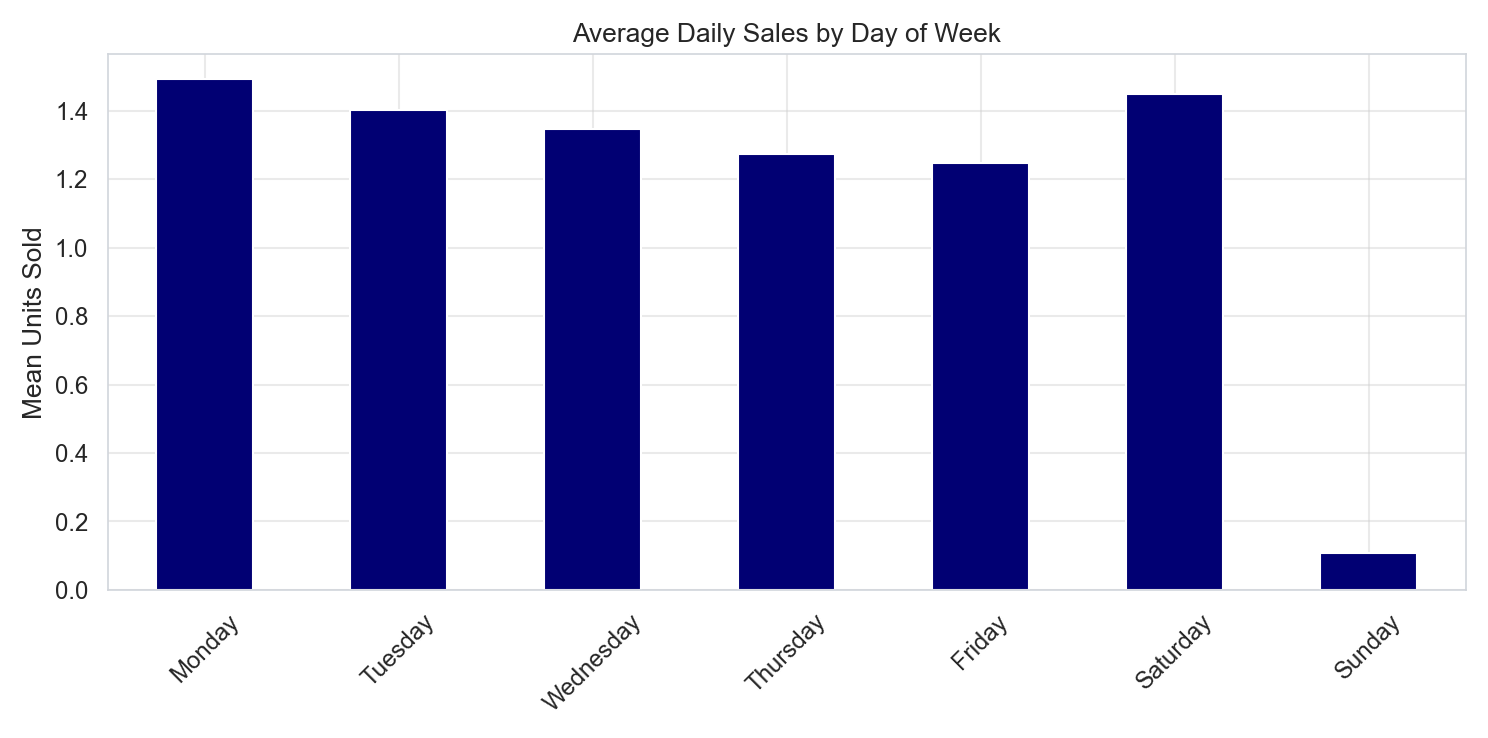
\includegraphics[width=0.85\textwidth]{figures/02_sales_by_day_of_week.png}
\caption{Average daily sales by day of the week. The weekly cycle is clearly visible, with near-zero sales on Sundays.}
\label{fig:sales_by_dow}
\end{figure}

\textbf{Monthly and seasonal patterns.} Monthly aggregated sales show moderate variation across the year, without a single dominant seasonal peak. However, certain months consistently show higher activity, suggesting that calendar-based features (month, week of year) may contribute predictive value.

\textbf{Promotional effects.} Comparing sales during promotional and non-promotional periods revealed that mean sales during promotions (1.83 units) were slightly higher than during non-promotional periods (1.38 units). However, the difference is modest, and the promotional flag alone does not capture the full complexity of promotional demand dynamics, which motivated the engineering of additional promotional features described in Section~3.4.

\begin{figure}[H]
\centering
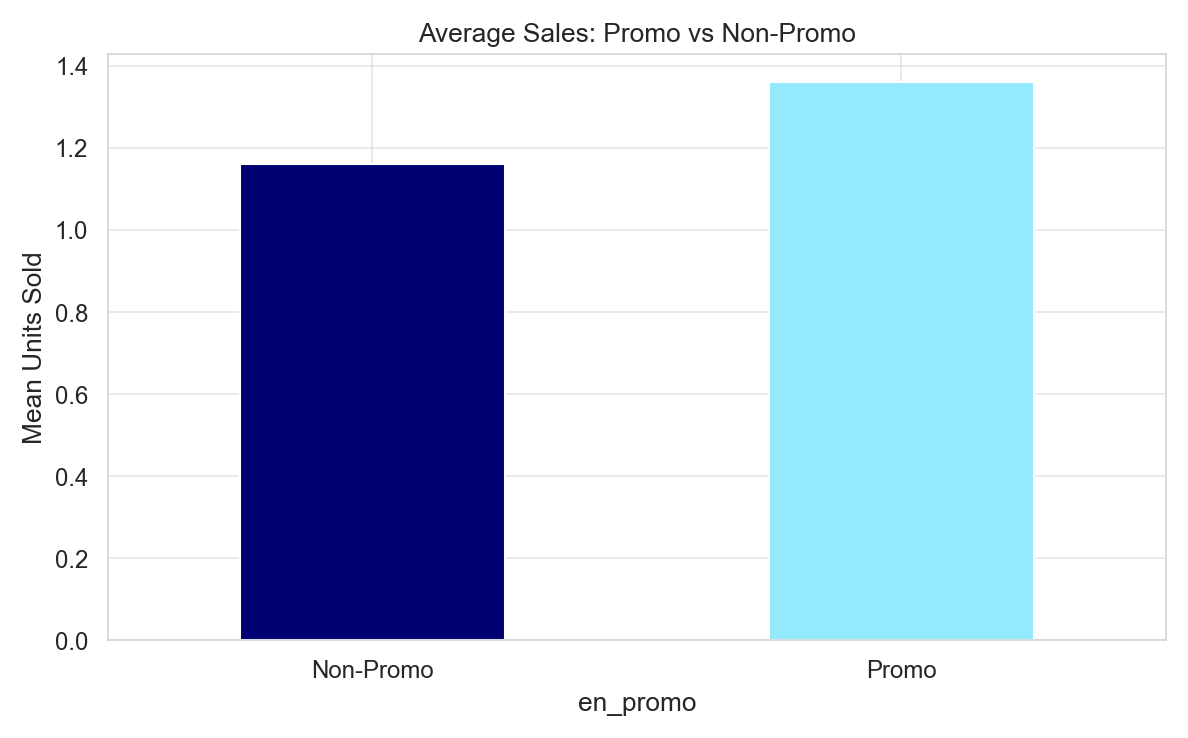
\includegraphics[width=0.85\textwidth]{figures/05_promo_vs_nonpromo.png}
\caption{Comparison of sales distributions during promotional and non-promotional periods.}
\label{fig:promo_vs_nonpromo}
\end{figure}

\textbf{Autocorrelation structure.} Autocorrelation analysis on a sample of products confirmed significant positive autocorrelation at lags 1, 7, 14, and 28, with the strongest signal at lag 7 (weekly periodicity). This finding directly supports the creation of lag features at these intervals and validates the choice of lag-7 as the naive baseline.

\begin{figure}[H]
\centering
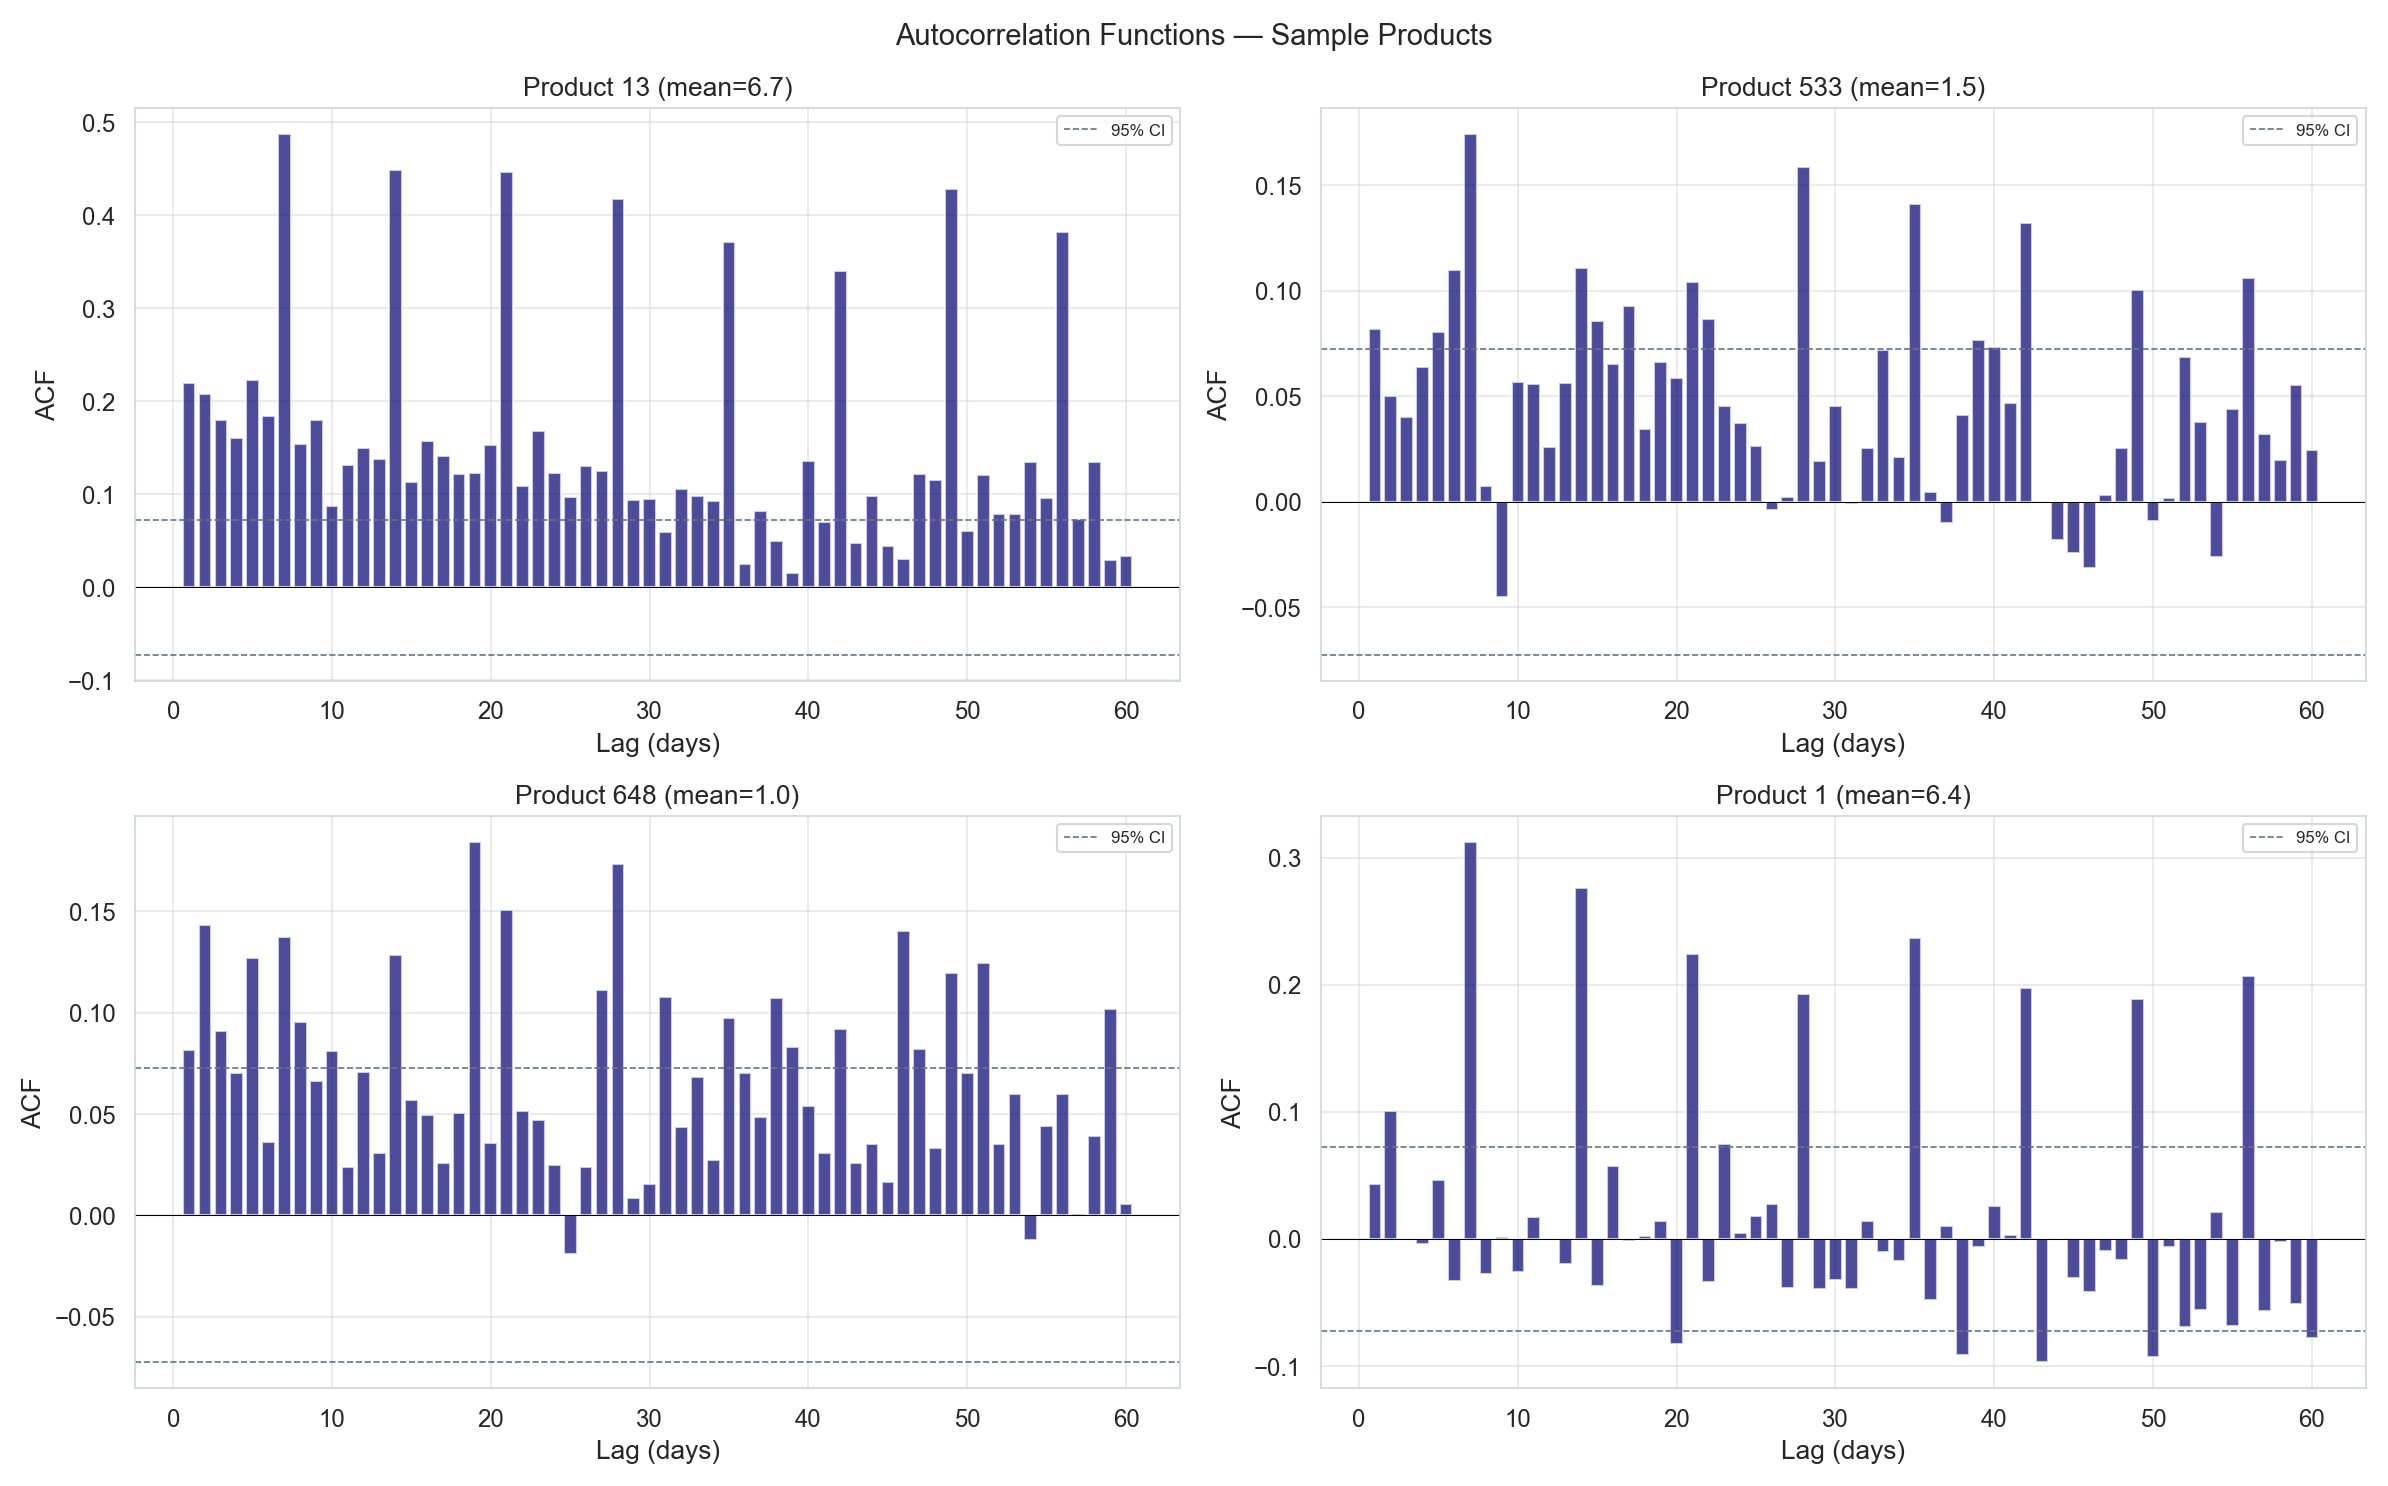
\includegraphics[width=0.85\textwidth]{figures/08_autocorrelation_sample.png}
\caption{Autocorrelation function (ACF) for a sample of products, showing significant positive autocorrelation at weekly intervals.}
\label{fig:autocorrelation}
\end{figure}

\subsection{Data Quality Analysis}

The data quality assessment identified the following issues:

\textbf{Missing values.} No explicit missing values were found in any of the four source tables. However, implicit gaps exist where lag features cannot be computed for the earliest dates in each product's history (addressed during feature engineering).

\textbf{Negative values.} No negative sales or stock values were present in this dataset.

\textbf{Stock breaks.} A stock break is defined as a day where both sales and stock are zero, potentially indicating that demand existed but could not be fulfilled due to inventory unavailability. Approximately 3.9\% of observations met this criterion. These were treated during data cleaning by imputing the product's historical mean sales for the corresponding weekday.

\textbf{Outliers.} Outlier detection was performed using a threshold of 1.75 times the interquartile range (IQR) per product. This identified approximately 11,400 observations (1.75\% of the dataset) as outliers, which were capped at the upper threshold value. The IQR-based approach was preferred over a fixed standard deviation threshold to account for the varying demand scales across products.


\section{Data Preparation}

\subsection{Data Cleaning}

The data cleaning process addressed the two quality issues identified during exploration:

\begin{enumerate}
    \item \textbf{Stock break imputation:} For observations where both \texttt{udsVenta} and \texttt{udsStock} were zero, the sales value was replaced with the mean sales for that product on the same weekday, computed over the preceding 30 days. This approach assumes that zero sales on a day with zero stock reflects a supply-side constraint rather than genuine zero demand, and uses a localised historical average to provide a reasonable demand estimate.

    \item \textbf{Outlier capping:} Values exceeding 1.75 $\times$ IQR above the 75th percentile for each product were capped at the threshold value. This preserves the general distribution shape while limiting the influence of extreme observations on model training. A total of 11,400 values (1.75\% of the dataset) were capped.
\end{enumerate}

After cleaning, the dataset retained its original 654,588 rows with no records removed, ensuring that the temporal continuity required for lag feature computation was preserved.

\subsection{Data Transformation}

The date column (\texttt{fecha}) was parsed into a \texttt{datetime} type, and the dataset was sorted by product and date to ensure correct temporal ordering for all subsequent operations. The promotional periods from the source data were transformed from date-range format into a daily binary indicator (\texttt{en\_promo}), assigned at the product-date level.

No logarithmic or power transformations were applied to the target variable. While such transformations can stabilise variance in skewed distributions, the tree-based models used in this work (Random Forest, XGBoost, LightGBM) are inherently robust to non-normal distributions and do not require target transformation for effective learning.

\subsection{Data Scaling}

Feature scaling (standardisation or normalisation) was not applied for the tree-based models, as decision tree ensembles are invariant to monotonic transformations of input features. The split-based learning mechanism of these algorithms operates on feature rankings rather than absolute values, making scaling unnecessary.

For the LSTM model, min-max normalisation was applied to all input features to facilitate gradient-based optimisation. Each feature was scaled to the $[0, 1]$ range using the training set statistics, and the same transformation was applied to the validation and test sets to prevent information leakage. Predictions were inverse-transformed back to the original scale before computing evaluation metrics.

\section{Feature Engineering}

Feature engineering is a central component of this work. A comprehensive set of 36 engineered features was designed to capture temporal dependencies, demand dynamics, and promotional effects. The features are organised into five categories, summarised in Table~\ref{tab:features}.

\begin{table}[H]
\centering
\small
\caption{Engineered features by category.}
\label{tab:features}
\begin{tabular}{|l|p{7cm}|r|}
\hline
\textbf{Category} & \textbf{Features} & \textbf{Count} \\
\hline
Original variables & udsStock, bolOpen, bolHoliday, en\_promo & 4 \\
\hline
Calendar features & year, month, day\_of\_week, week\_of\_year, week\_of\_month, is\_weekend, is\_month\_start, is\_month\_end & 8 \\
\hline
Lag features & lag\_1, lag\_7, lag\_14, lag\_28 & 4 \\
\hline
Rolling statistics & roll\_mean/std/min/max at 7, 14, and 28-day windows; ewma\_7, ewma\_28 & 14 \\
\hline
Promotional features & days\_since\_promo\_end, post\_promo\_7d, promo\_x\_lag7 & 3 \\
\hline
Product-level statistics & prod\_mean\_sales, prod\_std\_sales, prod\_median\_sales & 3 \\
\hline
\multicolumn{2}{|r|}{\textbf{Total}} & \textbf{36} \\
\hline
\end{tabular}
\end{table}

\textbf{Lag features} capture the autoregressive structure identified during exploration. The lag-7 feature (same weekday, previous week) serves dual purpose: it is used directly as the naive baseline forecast and as an input feature for the machine learning models. Lags at 1, 14, and 28 days capture short-term momentum, biweekly patterns, and monthly cycles respectively.

\textbf{Rolling statistics} provide smoothed representations of recent demand behaviour. For each window size (7, 14, and 28 days), the mean, standard deviation, minimum, and maximum of past sales are computed. Additionally, exponentially weighted moving averages (EWMA) with spans of 7 and 28 days provide adaptive smoothing that gives greater weight to more recent observations.

\textbf{Promotional features} go beyond the binary indicator to capture the temporal dynamics of promotions. The \texttt{days\_since\_promo\_end} feature tracks the recency of the last promotional period, \texttt{post\_promo\_7d} flags the week immediately following a promotion (to capture post-promotional demand depression), and \texttt{promo\_x\_lag7} is an interaction term between the promotional flag and the lag-7 sales value.

All lag and rolling features were computed strictly using past data to prevent information leakage. Observations where lag features could not be computed (the first 28 days of each product's history) were dropped, reducing the dataset from 654,588 to 629,370 rows. The final feature matrix was saved in Parquet format for use in the modelling phase.

\begin{figure}[H]
\centering
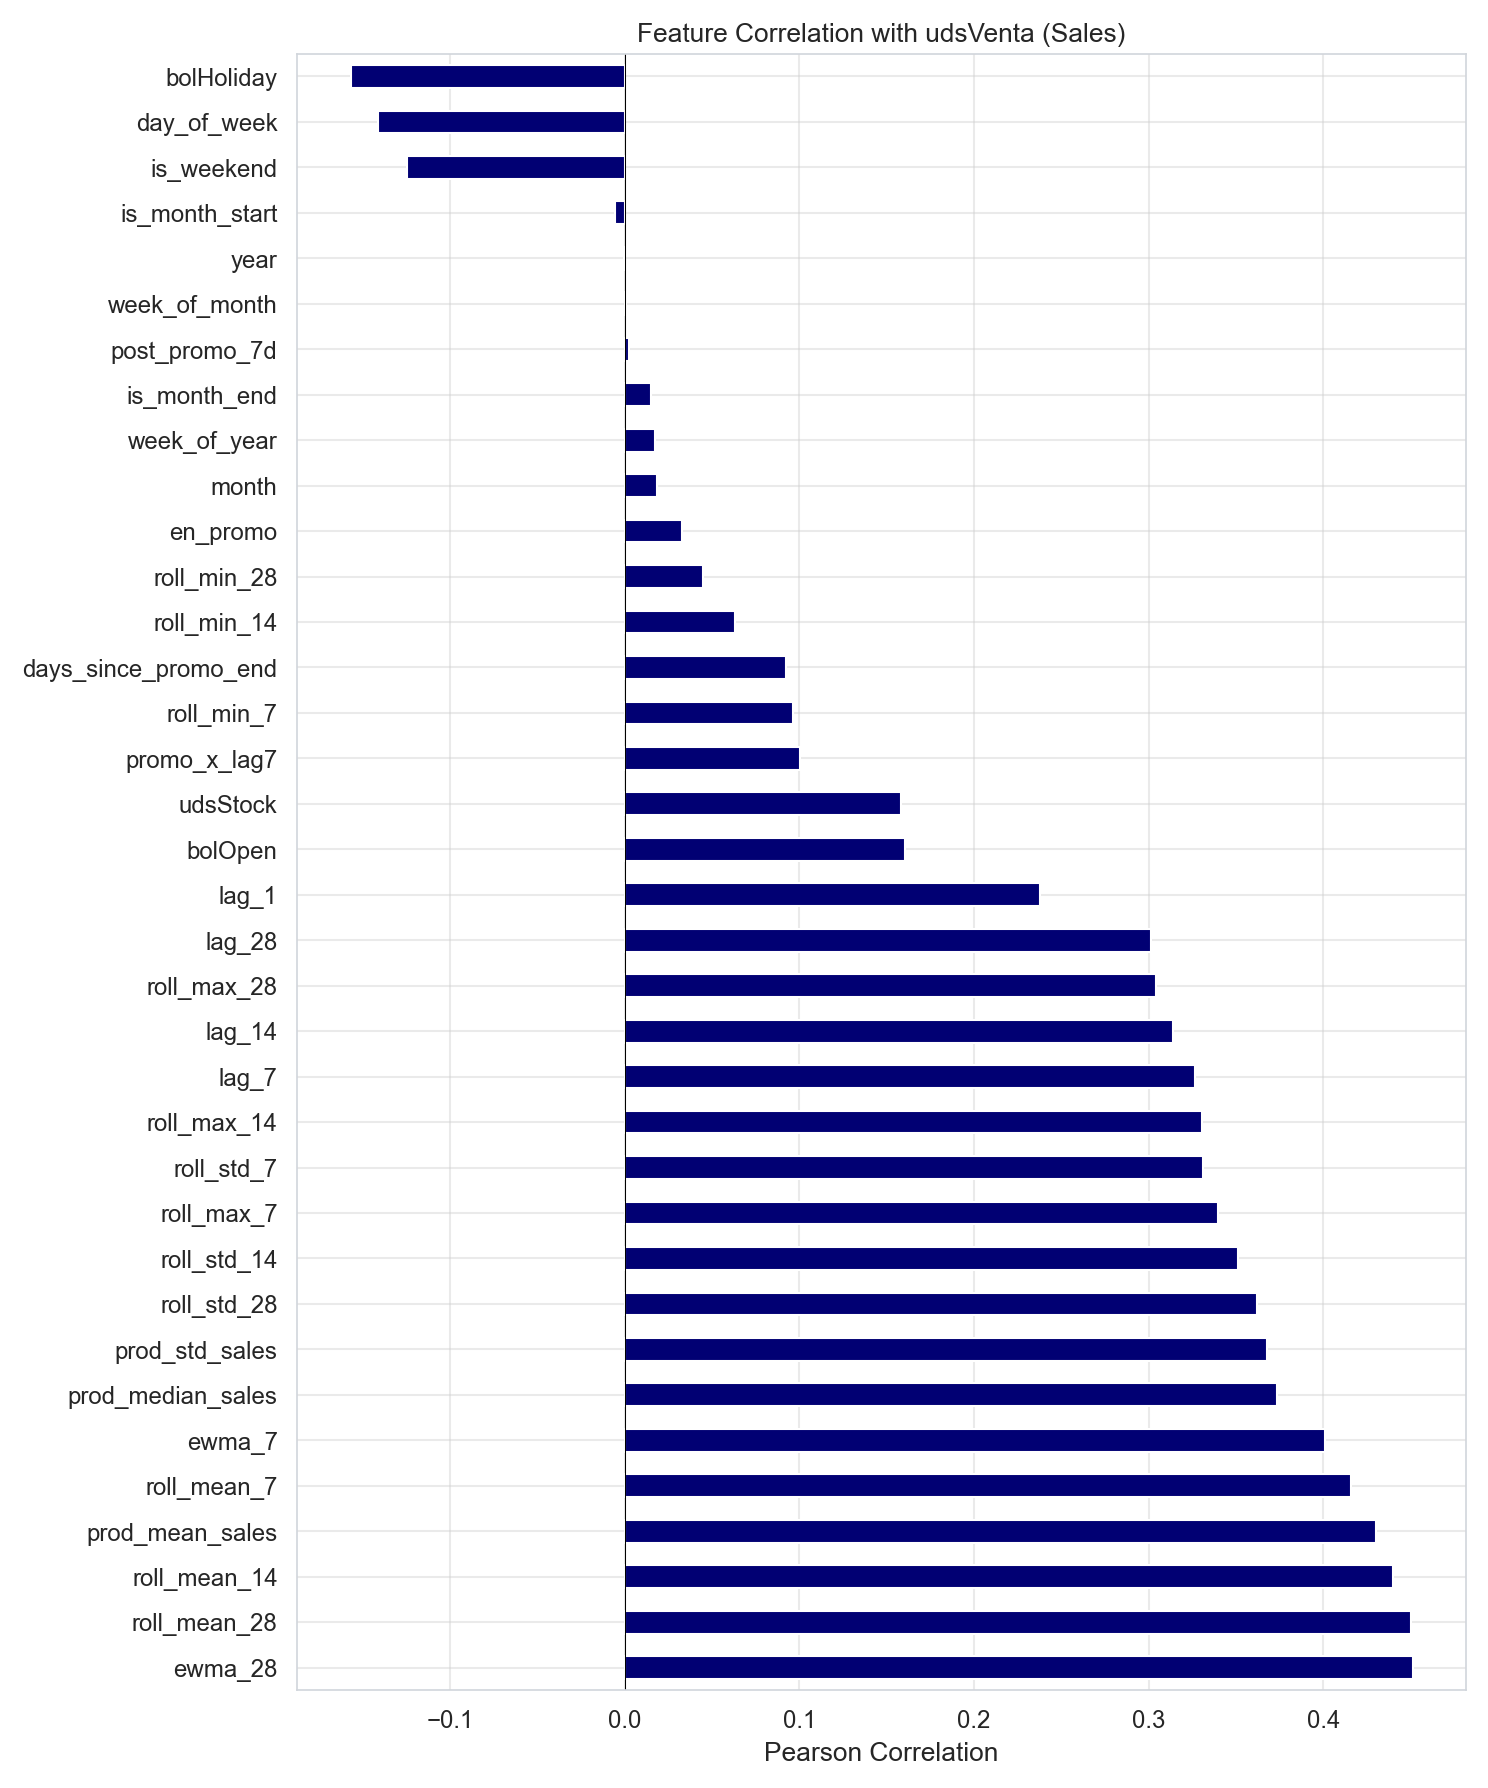
\includegraphics[width=0.95\textwidth]{figures/10_feature_correlations.png}
\caption{Correlation matrix of the engineered features. Strong correlations are visible among rolling statistics at different window sizes, confirming the presence of redundant but complementary temporal signals.}
\label{fig:feature_correlations}
\end{figure}


\section{Modelling}

\subsection{Model Selection}

Four forecasting approaches were implemented, spanning a naive baseline and three gradient boosting / ensemble methods:

\begin{enumerate}
    \item \textbf{Naive baseline (lag-7):} The simplest possible forecast, predicting that demand on any given day equals the demand observed on the same weekday of the previous week. This baseline exploits the strong weekly autocorrelation identified during exploration and provides a meaningful benchmark against which machine learning models must demonstrate improvement.

    \item \textbf{ARIMA (Seasonal):} A classical time series approach fitted per product using the \texttt{auto\_arima} implementation from the \texttt{pmdarima} library. Each product's demand series was modelled with seasonal ARIMA (SARIMA) with weekly periodicity ($m=7$), automatically selecting the optimal $(p,d,q)(P,D,Q)_7$ orders via stepwise search. ARIMA serves as the classical statistical baseline, representing the best that traditional time series methods can achieve without engineered features.

    \item \textbf{Random Forest:} An ensemble of decision trees trained on bootstrap samples with random feature subsets \citep{hyndman2021forecasting}. Random Forest provides robust predictions with built-in protection against overfitting through bagging and feature randomisation.

    \item \textbf{XGBoost:} A gradient boosting framework that builds trees sequentially, with each tree correcting the errors of its predecessors. XGBoost incorporates L1 and L2 regularisation, column subsampling, and efficient handling of sparse data, making it well-suited to the high proportion of zero-demand observations in this dataset.

    \item \textbf{LightGBM:} A gradient boosting implementation that uses histogram-based splitting and leaf-wise tree growth, offering faster training times than XGBoost while maintaining competitive accuracy. LightGBM was among the dominant algorithms in the M5 forecasting competition \citep{makridakis2021m5findings}.

    \item \textbf{LSTM (Long Short-Term Memory):} A recurrent neural network architecture designed to capture long-range temporal dependencies in sequential data \citep{hochreiter1997lstm}. Unlike tree-based methods, which rely on engineered lag features, LSTM processes input data as ordered sequences, with its internal gating mechanism allowing it to selectively retain or discard information from previous time steps. The model was implemented in PyTorch with a single LSTM layer (32 hidden units), trained on standardised features using 14-day input sequences.
\end{enumerate}

All tree-based models were trained on the full set of 33 input features (the 36 engineered features minus the 3 product-level statistics used only for reference). ARIMA was fitted per product on the raw sales series without engineered features, as is standard for classical time series methods. The LSTM model received the same 33 features as the tree models, but processed them as ordered sequences rather than independent observations. All predictions were clipped to a minimum of zero to prevent negative forecast values.

\subsection{Definition of Accuracy Indicators}

Four complementary metrics were used to evaluate forecast performance, as introduced in Chapter~2:

\begin{itemize}
    \item \textbf{MAE} (Mean Absolute Error): average absolute deviation between forecast and actual demand, in the same units as the target variable.
    \item \textbf{RMSE} (Root Mean Squared Error): penalises larger errors more heavily than MAE, providing a measure sensitive to occasional large deviations.
    \item \textbf{MAPE} (Mean Absolute Percentage Error): expresses errors as a percentage of actual demand, computed only for observations where actual demand is greater than zero to avoid division by zero.
    \item \textbf{$\sigma_e$} (forecast error standard deviation): the standard deviation of the residuals ($D_t - F_t$), which directly enters the safety stock calculation (Equation~\ref{eq:safety_stock}) and thus provides the link between forecast accuracy and inventory cost.
\end{itemize}

\subsection{Definition of Training and Validation Periods}

A rolling forecast origin validation strategy was adopted to provide a realistic assessment of out-of-sample performance by simulating the sequential nature of real forecasting decisions \citep{makridakis2021m5findings}.

Three validation folds were defined, each with a 30-day test window, working backwards from the most recent date in the dataset:

\begin{table}[H]
\centering
\small
\caption{Rolling forecast origin validation folds.}
\label{tab:folds}
\begin{tabular}{|c|c|c|c|}
\hline
\textbf{Fold} & \textbf{Training period end} & \textbf{Test period} & \textbf{Test days} \\
\hline
1 & 2024-09-06 & 2024-09-07 -- 2024-10-06 & 30 \\
2 & 2024-10-06 & 2024-10-07 -- 2024-11-05 & 30 \\
3 & 2024-10-06 & 2024-10-07 -- 2024-11-05 & 30 \\
\hline
\end{tabular}
\end{table}

For each fold, the training set includes all data up to the fold's cutoff date (expanding window), and the model is evaluated on the subsequent 30-day period. Final reported metrics are averaged across all three folds.

\subsection{Hyperparameter Tuning}

Hyperparameters for all three machine learning models were optimised using Optuna \citep{makridakis2021m5findings}, a Bayesian optimisation framework that efficiently explores the parameter space using a Tree-structured Parzen Estimator (TPE) sampler.

To balance computational cost with tuning quality, the optimisation was conducted on a representative subset of 50 randomly sampled products using the first validation fold. Each model was allocated 30 Optuna trials, with RMSE on the validation set as the objective function. The optimised hyperparameters were then applied to the full dataset across all validation folds.

Table~\ref{tab:tuned_params} presents the key tuned hyperparameters for each model:

\begin{table}[H]
\centering
\small
\caption{Optimised hyperparameters via Optuna (30 trials per model).}
\label{tab:tuned_params}
\begin{tabular}{|l|l|r|}
\hline
\textbf{Model} & \textbf{Parameter} & \textbf{Value} \\
\hline
\multirow{5}{*}{LightGBM} & n\_estimators & 300 \\
 & learning\_rate & 0.011 \\
 & num\_leaves & 75 \\
 & max\_depth & 4 \\
 & min\_child\_samples & 25 \\
\hline
\multirow{5}{*}{XGBoost} & n\_estimators & 350 \\
 & learning\_rate & 0.019 \\
 & max\_depth & 3 \\
 & min\_child\_weight & 10 \\
 & subsample & 0.90 \\
\hline
\multirow{4}{*}{Random Forest} & n\_estimators & 100 \\
 & max\_depth & 5 \\
 & min\_samples\_leaf & 16 \\
 & max\_features & 0.30 \\
\hline
\end{tabular}
\end{table}

The relatively shallow tree depths (3--5) and conservative learning rates (0.011--0.019) selected by the optimiser suggest that the models benefit from regularisation, which is consistent with the high proportion of zero-demand observations in the dataset.


\section{Evaluation}

\subsection{Accuracy Results Obtained}

Table~\ref{tab:results_summary} presents the average performance of each model across the three validation folds:

\begin{table}[H]
\centering
\small
\caption{Average forecast accuracy across three rolling validation folds.}
\label{tab:results_summary}
\begin{tabular}{|l|r|r|r|r|}
\hline
\textbf{Model} & \textbf{MAE} & \textbf{RMSE} & \textbf{MAPE (\%)} & \textbf{$\sigma_e$} \\
\hline
XGBoost & 1.366 & 2.155 & 52.2 & 2.154 \\
LightGBM & 1.373 & 2.158 & 51.7 & 2.158 \\
Random Forest & 1.394 & 2.176 & 51.6 & 2.176 \\
ARIMA$^\dagger$ & 1.443 & 2.220 & 59.8 & 2.219 \\
LSTM & 1.522 & 2.235 & 49.8 & 2.223 \\
Naive (lag-7) & 1.661 & 3.091 & 86.0 & 3.091 \\
\hline
\end{tabular}
\begin{flushleft}
\footnotesize{$^\dagger$ ARIMA evaluated on 50 sampled products due to per-product fitting cost.}
\end{flushleft}
\end{table}

All three tree-based machine learning models substantially outperform both the naive baseline and the classical/deep learning alternatives. XGBoost achieves the lowest RMSE (2.155), followed closely by LightGBM (2.158) and Random Forest (2.176). The RMSE improvement over the naive baseline ranges from 27.9\% (LSTM) to 30.3\% (XGBoost).

\begin{figure}[H]
\centering
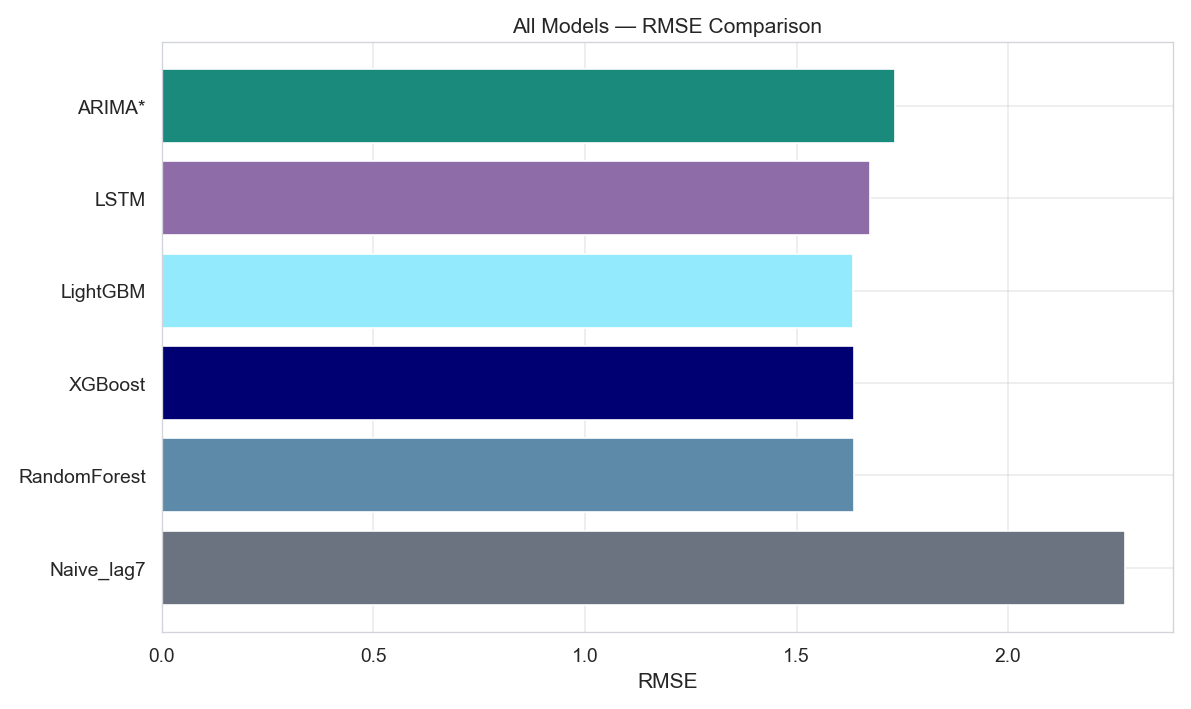
\includegraphics[width=0.85\textwidth]{figures/24_all_models_comparison.png}
\caption{Comparison of forecast accuracy (RMSE) across all six models. The three tree-based models form a tight cluster, substantially outperforming both classical and deep learning alternatives.}
\label{fig:all_models_comparison}
\end{figure}

ARIMA and LSTM occupy an intermediate position: both significantly outperform the naive baseline (RMSE reductions of 28.2\% and 27.7\% respectively) but fall short of the tree-based models. This result is consistent with the findings of the M5 forecasting competition \citep{makridakis2021m5findings}, where gradient boosting algorithms consistently outperformed both classical statistical methods and standalone deep learning approaches. The LSTM's slightly lower MAPE (49.8\%) but higher RMSE suggests it handles the zero-heavy distribution differently from tree models, producing fewer large percentage errors but occasionally larger absolute deviations.

\subsection{Comparison of Results Across Models}

\textbf{Promotional vs. non-promotional performance.} Table~\ref{tab:promo_results} compares model performance across demand segments:

\begin{table}[H]
\centering
\small
\caption{Model performance by demand segment (last validation fold).}
\label{tab:promo_results}
\begin{tabular}{|l|l|r|r|r|r|}
\hline
\textbf{Segment} & \textbf{Model} & \textbf{MAE} & \textbf{RMSE} & \textbf{MAPE (\%)} & \textbf{$\sigma_e$} \\
\hline
\multirow{4}{*}{Non-Promo} & XGBoost & 1.299 & 2.055 & 52.3 & 2.055 \\
 & LightGBM & 1.308 & 2.058 & 51.8 & 2.058 \\
 & Random Forest & 1.327 & 2.073 & 51.6 & 2.073 \\
 & Naive (lag-7) & 1.565 & 2.969 & 85.9 & 2.969 \\
\hline
\multirow{4}{*}{Promo} & XGBoost & 1.917 & 2.844 & 51.7 & 2.836 \\
 & LightGBM & 1.911 & 2.851 & 51.4 & 2.838 \\
 & Random Forest & 1.944 & 2.884 & 51.6 & 2.873 \\
 & Naive (lag-7) & 2.448 & 3.956 & 86.9 & 3.955 \\
\hline
\end{tabular}
\end{table}

Promotional demand is consistently harder to predict across all models, with RMSE values approximately 38\% higher than for non-promotional periods. However, the ML models maintain their advantage over the naive baseline in both segments, with RMSE improvements of approximately 28\% for non-promotional and 28\% for promotional demand.

\textbf{Per-product RMSE distribution.} Analysis at the individual product level reveals that LightGBM achieves a median per-product RMSE of 1.65, compared to 2.36 for the naive baseline. The improvement is not uniform: some products see RMSE reductions exceeding 15 units, while approximately 10 products show marginally worse performance with ML than with the naive approach. These products tend to have very low and stable demand where the simple lag-7 heuristic is already near-optimal.

\begin{figure}[H]
\centering
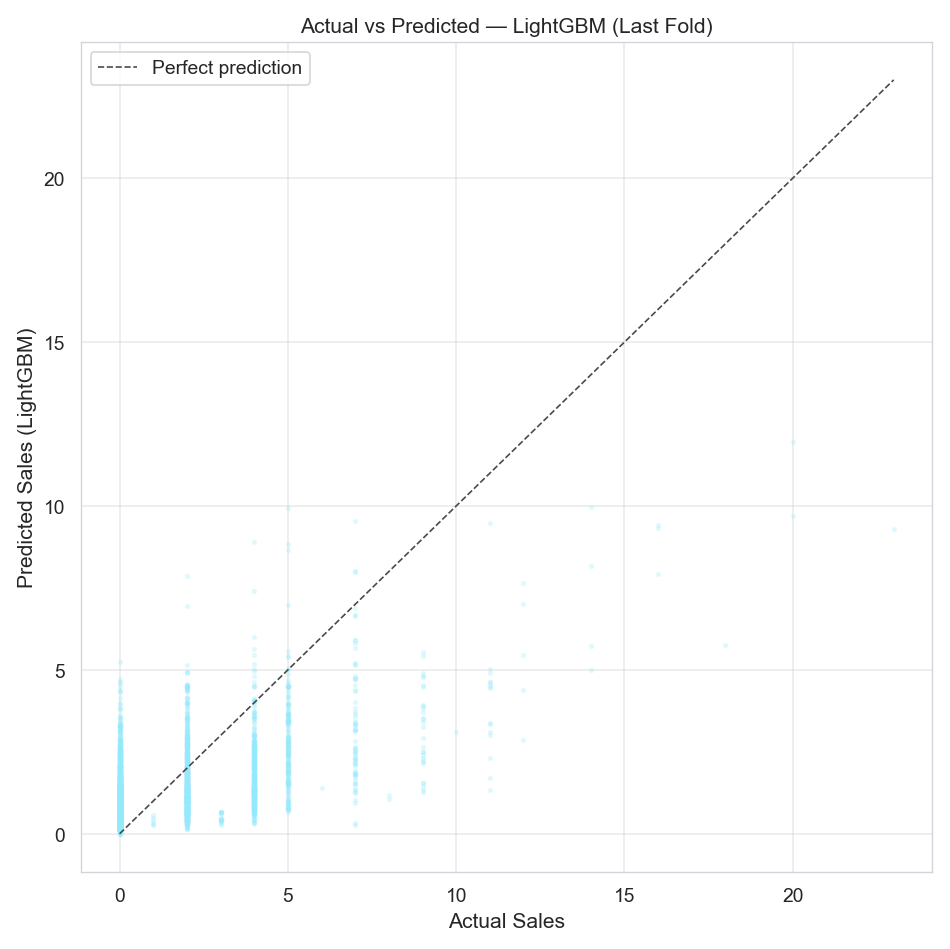
\includegraphics[width=0.85\textwidth]{figures/13_actual_vs_predicted_lgbm.png}
\caption{Actual vs.\ predicted sales for LightGBM on a sample of products. Points near the diagonal indicate accurate predictions; the cluster near the origin reflects the high proportion of zero-demand observations.}
\label{fig:actual_vs_predicted}
\end{figure}

\begin{figure}[H]
\centering
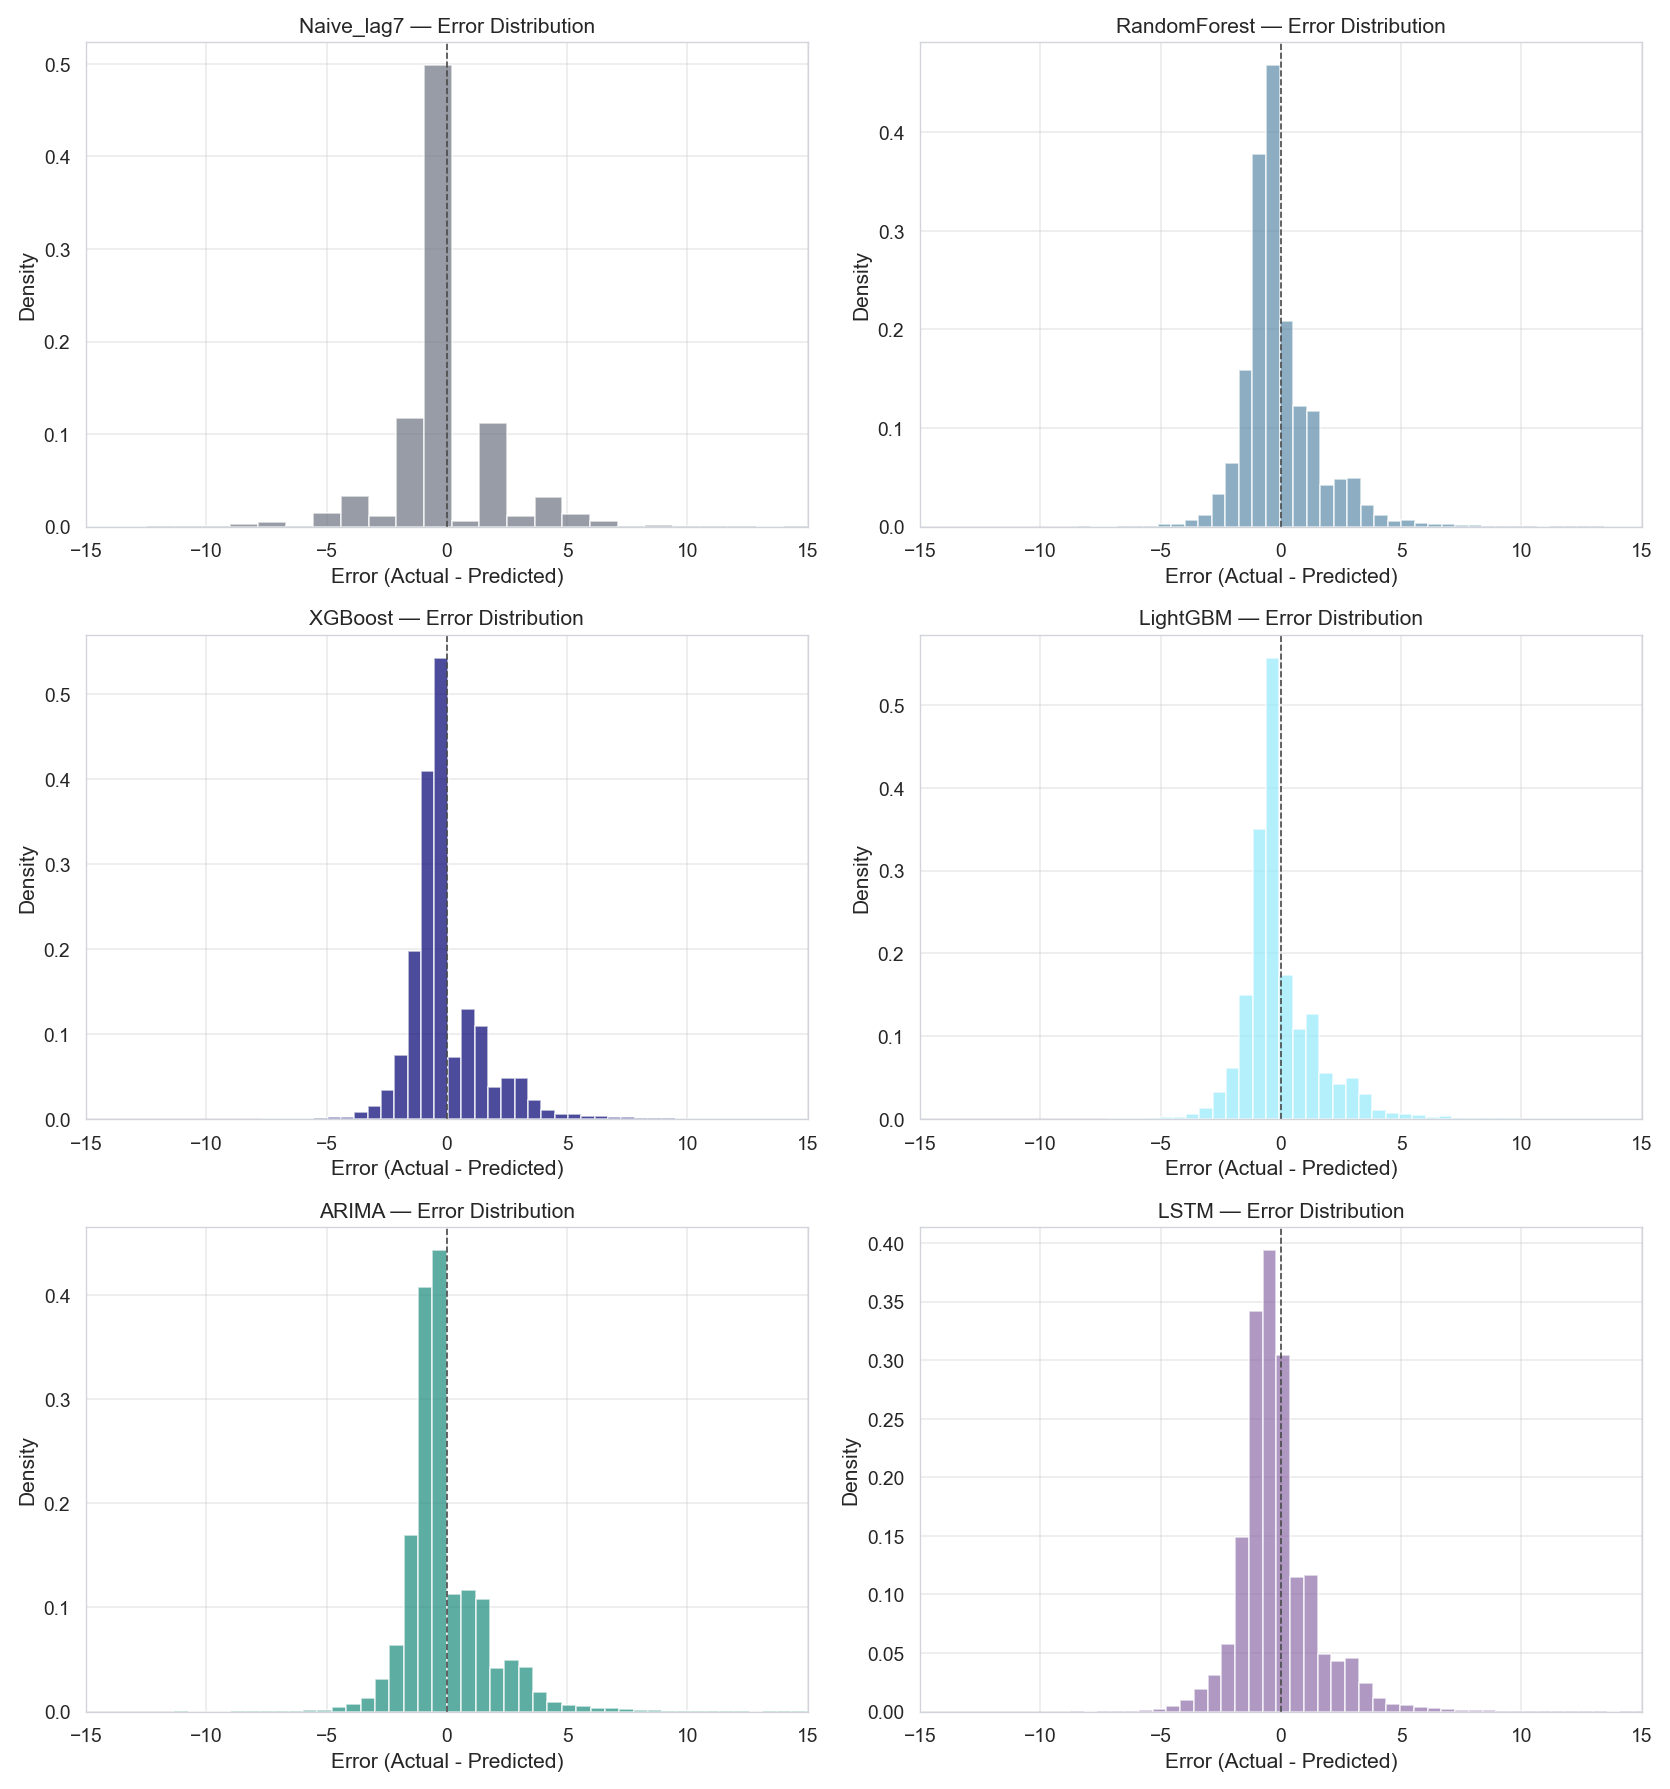
\includegraphics[width=0.85\textwidth]{figures/17_error_distributions.png}
\caption{Distribution of forecast errors by model. The ML models produce tighter, more symmetric error distributions compared to the naive baseline.}
\label{fig:error_distributions}
\end{figure}

\begin{figure}[H]
\centering
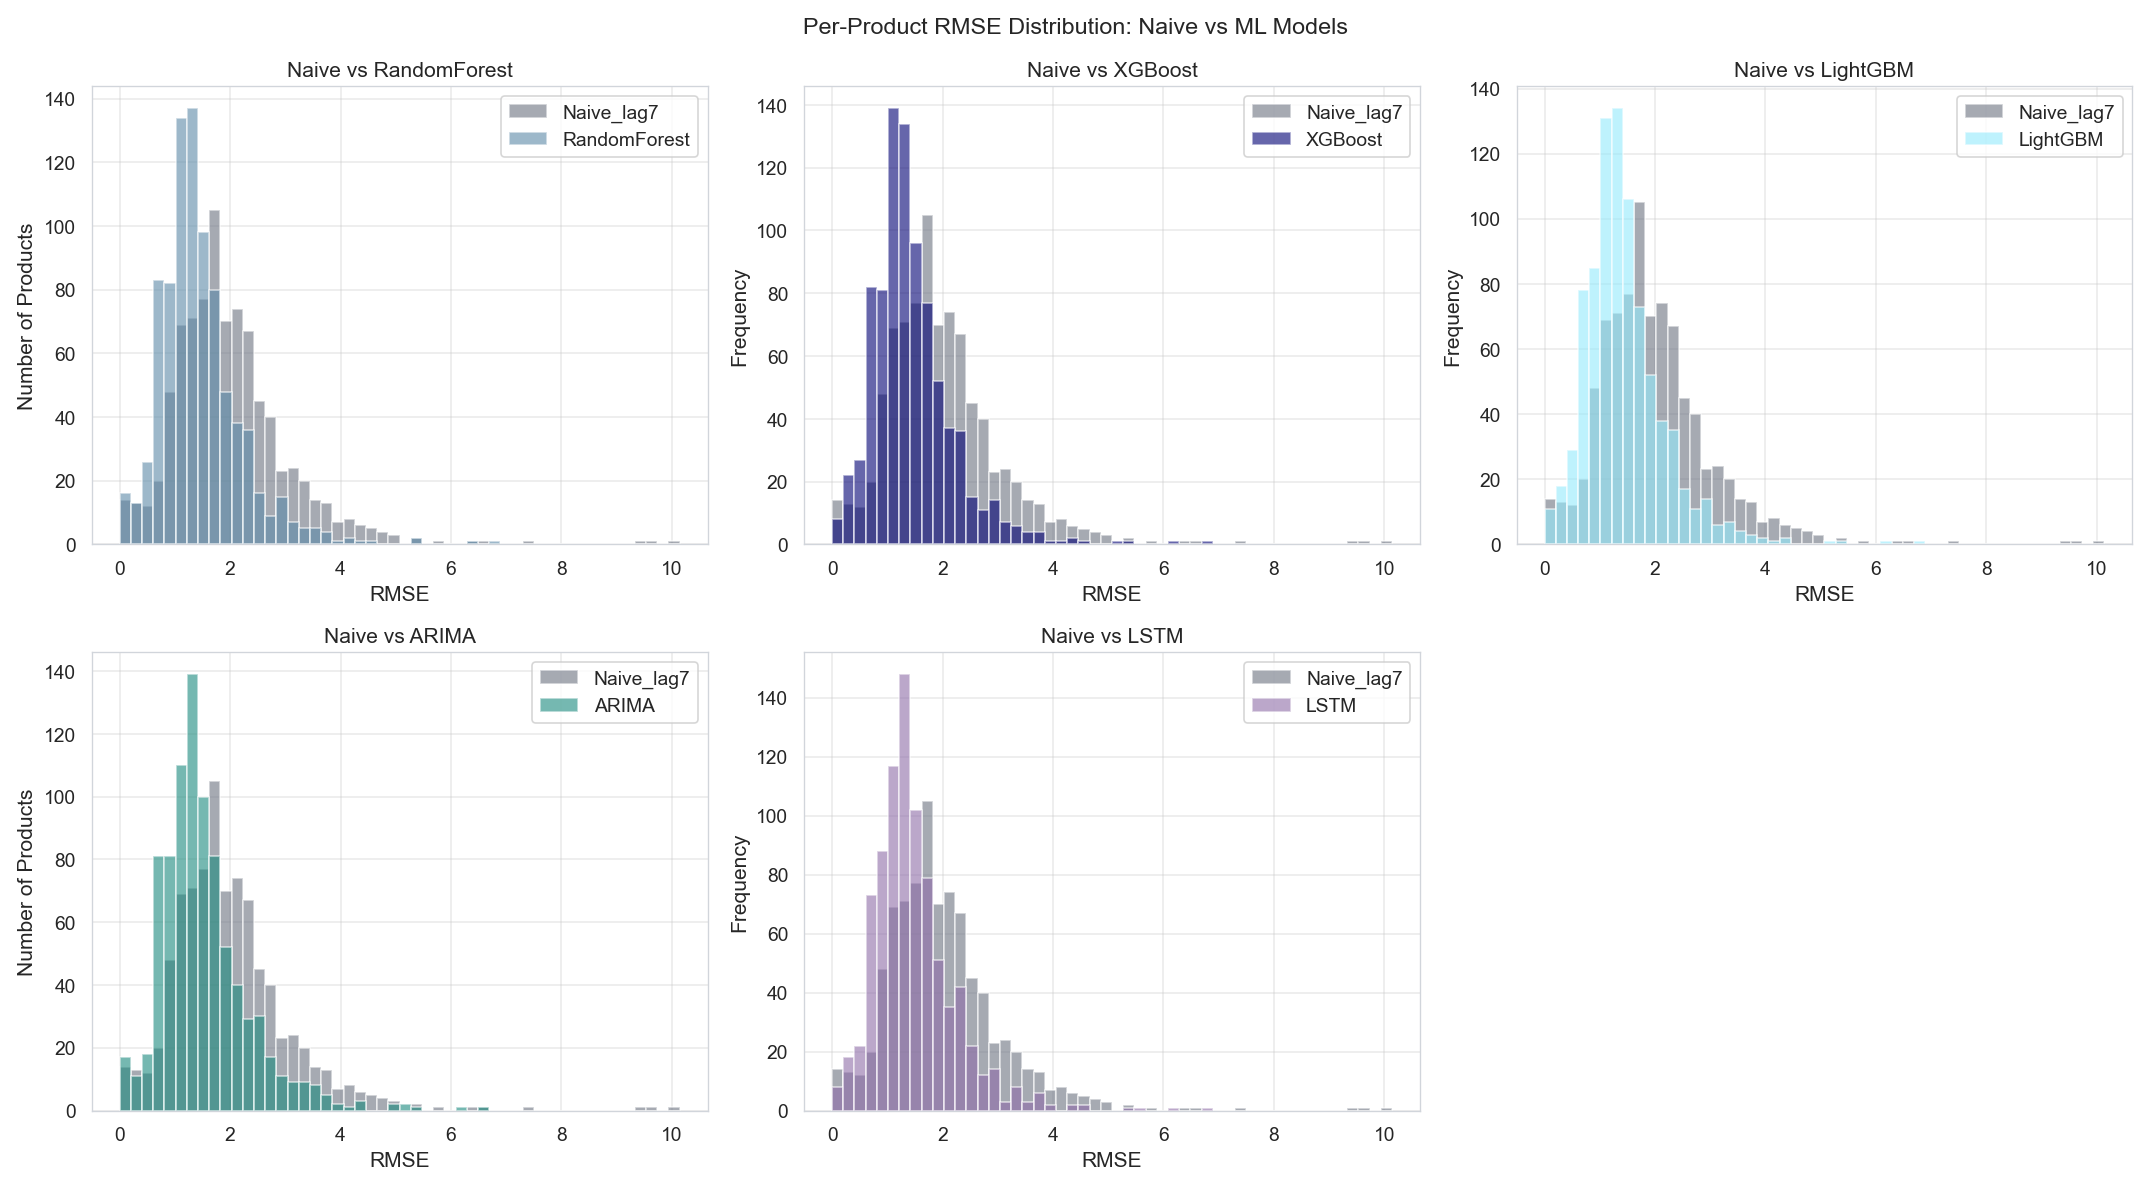
\includegraphics[width=0.85\textwidth]{figures/18_per_product_rmse_dist.png}
\caption{Distribution of per-product RMSE values. The ML models shift the distribution towards lower RMSE values compared to the naive baseline.}
\label{fig:per_product_rmse}
\end{figure}

\textbf{SHAP feature importance.} To understand the drivers of model predictions, SHAP (SHapley Additive exPlanations) analysis was performed on the LightGBM model. Table~\ref{tab:shap_top10} presents the ten most influential features:

\begin{table}[H]
\centering
\small
\caption{Top 10 features by mean absolute SHAP value (LightGBM).}
\label{tab:shap_top10}
\begin{tabular}{|r|l|r|}
\hline
\textbf{Rank} & \textbf{Feature} & \textbf{Mean $|$SHAP$|$} \\
\hline
1 & ewma\_28 & 0.524 \\
2 & bolHoliday & 0.295 \\
3 & roll\_mean\_28 & 0.150 \\
4 & day\_of\_week & 0.079 \\
5 & udsStock & 0.063 \\
6 & roll\_max\_28 & 0.046 \\
7 & lag\_28 & 0.025 \\
8 & bolOpen & 0.022 \\
9 & roll\_mean\_14 & 0.017 \\
10 & roll\_max\_14 & 0.016 \\
\hline
\end{tabular}
\end{table}

The 28-day EWMA emerges as the single most important predictor, followed by the holiday indicator and the 28-day rolling mean. This confirms that the model relies heavily on smoothed representations of recent demand history, with calendar effects providing secondary but significant predictive power. Notably, the longer-horizon features (28-day windows) dominate over shorter-horizon ones (7-day), suggesting that the model captures medium-term demand trends rather than relying solely on short-term momentum.

\begin{figure}[H]
\centering
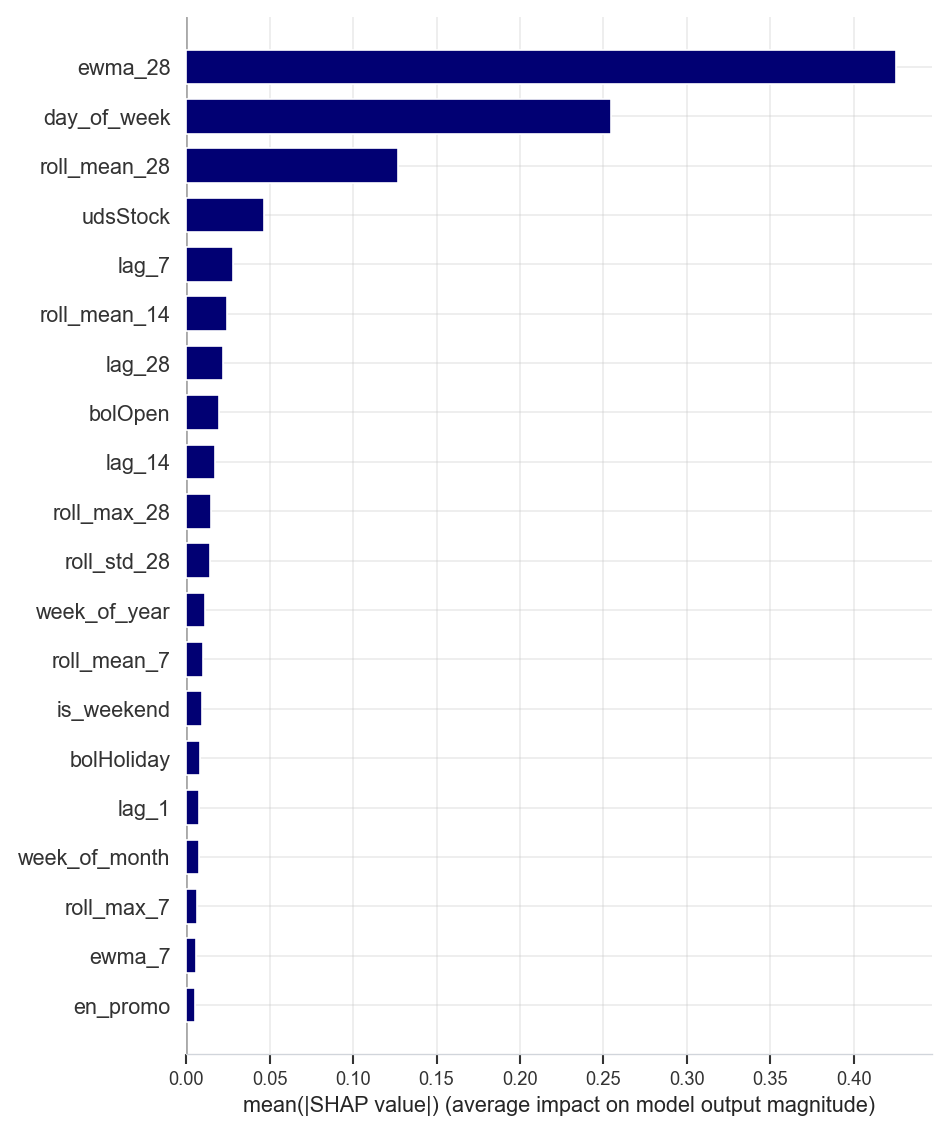
\includegraphics[width=0.85\textwidth]{figures/15_shap_bar.png}
\caption{SHAP feature importance (mean absolute SHAP values) for LightGBM. The 28-day EWMA dominates, followed by calendar and rolling statistics features.}
\label{fig:shap_bar}
\end{figure}

\begin{figure}[H]
\centering
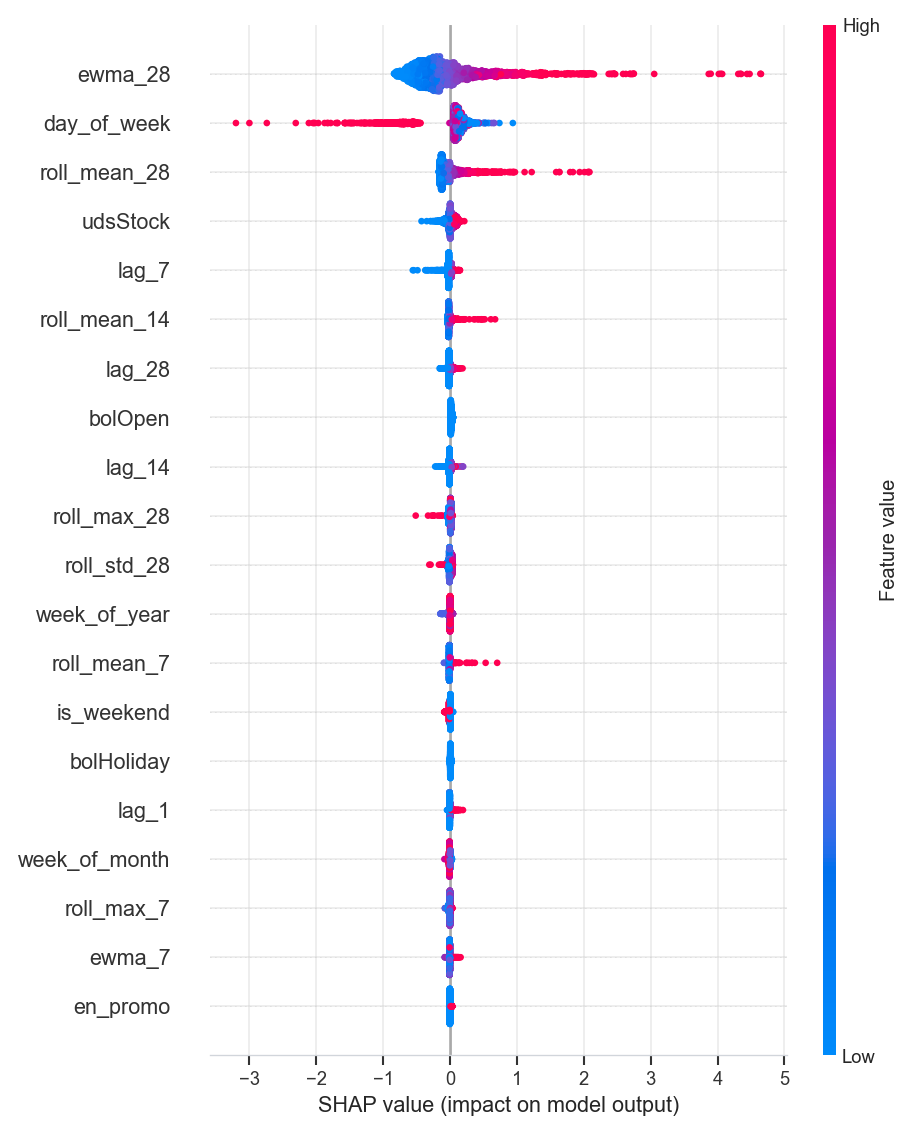
\includegraphics[width=0.85\textwidth]{figures/14_shap_summary.png}
\caption{SHAP summary plot showing the direction and magnitude of feature effects. Red indicates high feature values; blue indicates low values. High \texttt{ewma\_28} values push predictions upward, consistent with higher recent demand leading to higher forecasts.}
\label{fig:shap_summary}
\end{figure}

\subsection{Conclusions from Results}

The evaluation yields several key findings:

\begin{enumerate}
    \item The three tree-based machine learning models (XGBoost, LightGBM, Random Forest) achieve the best performance, with RMSE values within 1\% of each other. This suggests that the feature engineering, rather than the specific algorithm choice, is the primary driver of forecast quality among this model family.

    \item ARIMA and LSTM occupy an intermediate tier, both significantly outperforming the naive baseline (RMSE reductions of 28\% and 28\% respectively) but falling short of the tree-based models. ARIMA's per-product fitting captures local demand patterns effectively but cannot leverage cross-product information or engineered features. LSTM captures sequential dependencies but requires substantially more training data and computation to match tree-based performance.

    \item The improvement over the naive baseline is substantial across all ML approaches (28--30\% RMSE reduction), demonstrating the value of incorporating engineered features and systematic model training over simple heuristic forecasting.

    \item Promotional demand remains the most challenging segment, with RMSE approximately 38\% higher than non-promotional demand across all models. However, the ML models maintain their relative advantage over the baseline in both segments.

    \item SHAP analysis reveals that smoothed demand history (EWMA and rolling statistics) and calendar features are the most influential predictors, validating the feature engineering strategy adopted in this work.

    \item The forecast error standard deviation ($\sigma_e \approx 2.15$ for the best tree models, $\sigma_e \approx 2.22$ for ARIMA/LSTM, compared to $\sigma_e \approx 3.09$ for the naive baseline) translates directly into safety stock reductions, as quantified in the following section.
\end{enumerate}


\section{Impact of Algorithm Improvement}

\subsection{Impact on Processes}

The transition from a naive forecasting approach to machine learning models has implications beyond numerical accuracy improvements. From an operational perspective, the key process impacts are:

\textbf{Safety stock reduction.} Using the safety stock formulation from Equation~\ref{eq:safety_stock} with a 95\% service level ($z = 1.645$) and a protection period of 10 days (3 days lead time + 7 days review period), the total safety stock across all 894 products decreases from 11,953 units under the naive forecast to 8,276 units under LightGBM --- a reduction of 30.8\%. This means that the same service level can be maintained with significantly less inventory investment.

\textbf{Forecast error symmetry.} Analysis of error distributions shows that the ML models produce approximately symmetric errors centred near zero, whereas the naive baseline exhibits a slight positive bias (tendency to overforecast). Symmetric errors are preferable for inventory planning, as they indicate that the forecast is equally likely to overestimate or underestimate demand, allowing safety stock to function as intended.

\textbf{Sensitivity to service level.} Table~\ref{tab:sensitivity} presents the total safety stock requirements across different service levels:

\begin{table}[H]
\centering
\small
\caption{Total safety stock (units) by model and service level.}
\label{tab:sensitivity}
\begin{tabular}{|l|r|r|r|}
\hline
\textbf{Model} & \textbf{90\%} & \textbf{95\%} & \textbf{99\%} \\
\hline
LightGBM & 6,450 & 8,276 & 11,702 \\
XGBoost & 6,466 & 8,296 & 11,731 \\
Random Forest & 6,507 & 8,350 & 11,806 \\
Naive (lag-7) & 9,316 & 11,953 & 16,902 \\
\hline
\end{tabular}
\end{table}

The ML models consistently require approximately 30\% less safety stock than the naive baseline across all service levels, demonstrating that the improvement is robust and not dependent on a specific service level assumption.

\begin{figure}[H]
\centering
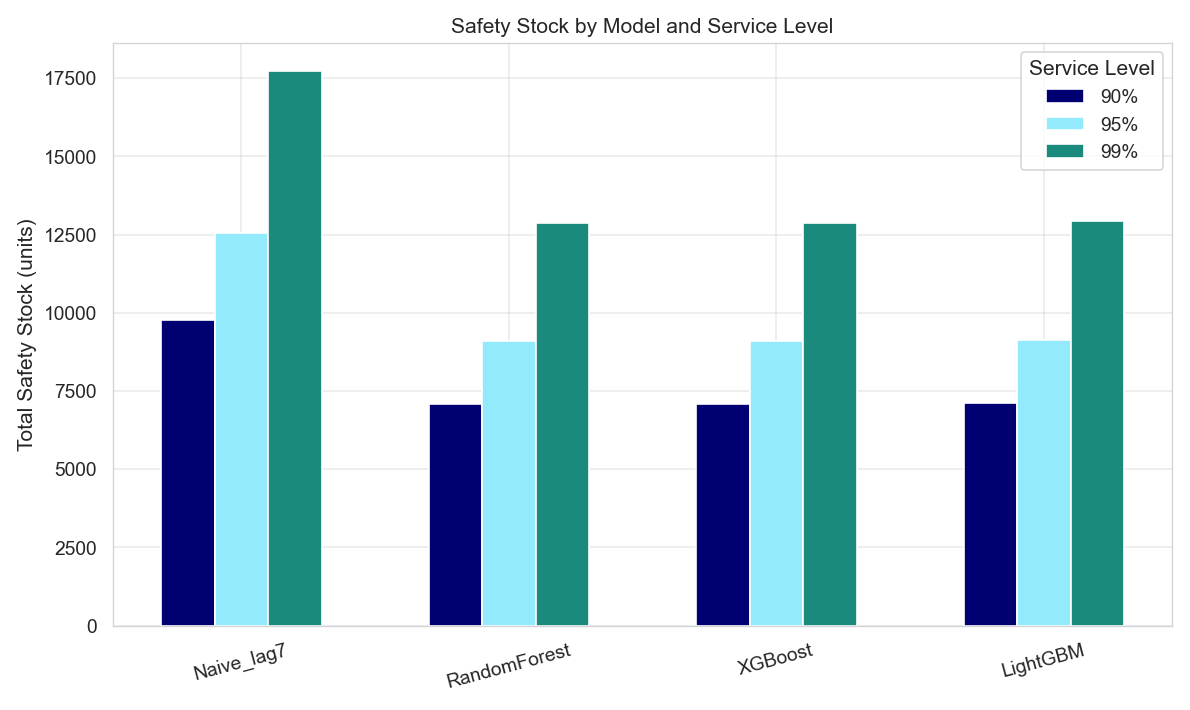
\includegraphics[width=0.85\textwidth]{figures/21_safety_stock_by_service_level.png}
\caption{Total safety stock requirements by model and service level. The ML models maintain a consistent ~30\% advantage over the naive baseline across all service levels.}
\label{fig:safety_stock_service_level}
\end{figure}

\subsection{Economic Impact}

The economic impact analysis combines two cost components: the newsvendor cost (direct cost of forecast errors) and the safety stock holding cost.

\textbf{Newsvendor cost analysis.} Following the total cost formulation from Equation~\ref{eq:total_cost}, the asymmetric costs of overforecasting and underforecasting were computed using cost parameters of $C_o = \text{\euro}0.10$ per unit per day (overage/holding) and $C_u = \text{\euro}0.50$ per unit per day (underage/lost sale), yielding a critical ratio of 0.83. These values reflect a typical retail/industrial setting where stockout costs substantially exceed holding costs.

Table~\ref{tab:newsvendor} presents the newsvendor cost results:

\begin{table}[H]
\centering
\small
\caption{Newsvendor cost analysis (30-day test period, annualised).}
\label{tab:newsvendor}
\begin{tabular}{|l|r|r|r|r|}
\hline
\textbf{Model} & \textbf{Overage (€)} & \textbf{Underage (€)} & \textbf{Total (€)} & \textbf{Annual est. (€)} \\
\hline
Naive (lag-7) & 2,227 & 11,138 & 13,365 & 162,603 \\
Random Forest & 1,830 & 9,538 & 11,367 & 138,304 \\
LightGBM & 1,786 & 9,489 & 11,275 & 137,182 \\
XGBoost & 1,785 & 9,392 & 11,176 & 135,979 \\
\hline
\end{tabular}
\end{table}

XGBoost achieves the lowest newsvendor cost, saving approximately \euro26,600 annually (16.4\%) compared to the naive baseline. Underage costs dominate in all models, consistent with the asymmetric cost structure where stockouts are five times more expensive than excess inventory.

\textbf{Combined cost analysis.} Table~\ref{tab:combined_cost} presents the total annual cost combining newsvendor costs with safety stock holding costs at the 95\% service level:

\begin{table}[H]
\centering
\small
\caption{Combined annual cost: newsvendor + safety stock holding (95\% service level).}
\label{tab:combined_cost}
\begin{tabular}{|l|r|r|r|}
\hline
\textbf{Model} & \textbf{Newsvendor (€/yr)} & \textbf{SS Holding (€/yr)} & \textbf{Total (€/yr)} \\
\hline
Naive (lag-7) & 162,603 & 436,294 & 598,896 \\
Random Forest & 138,304 & 304,763 & 443,067 \\
LightGBM & 137,182 & 302,083 & 439,265 \\
XGBoost & 135,979 & 302,816 & 438,796 \\
\hline
\end{tabular}
\end{table}

The ML models achieve total annual cost savings of approximately \euro160,000 (26.7\%) compared to the naive baseline. XGBoost and LightGBM perform nearly identically in economic terms, with XGBoost holding a marginal advantage of \euro469 annually.

\begin{figure}[H]
\centering
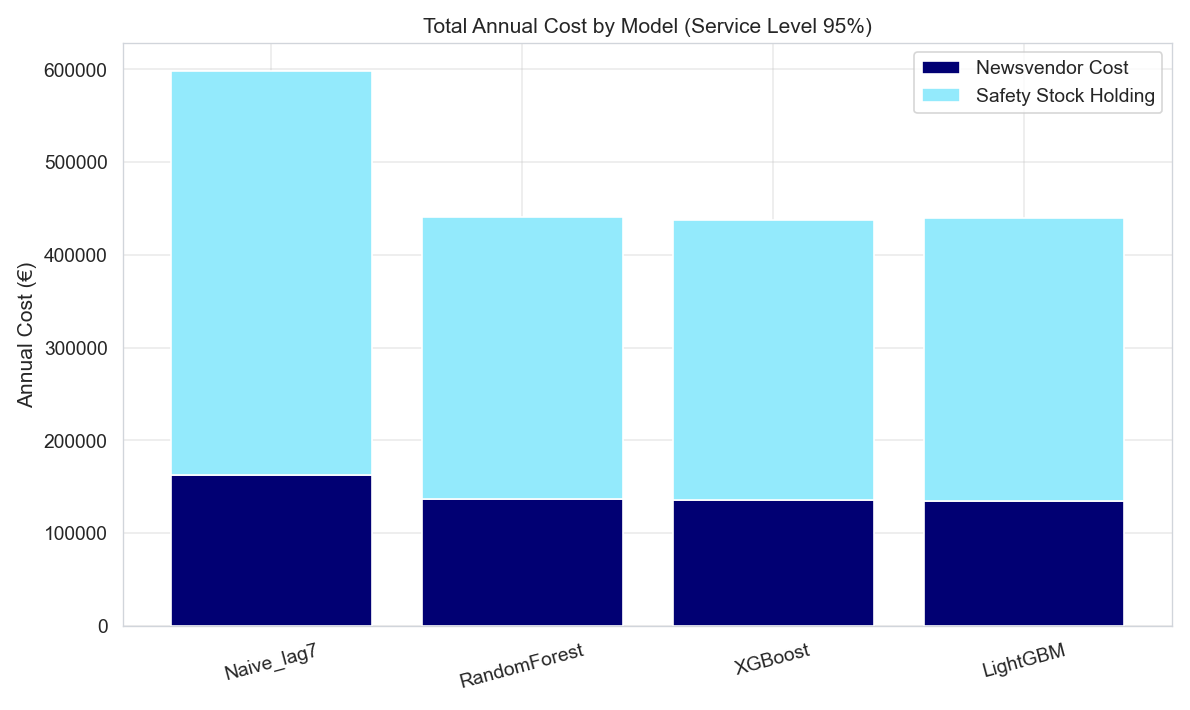
\includegraphics[width=0.85\textwidth]{figures/22_combined_annual_cost.png}
\caption{Combined annual inventory cost (newsvendor + safety stock holding) by model. The ML models reduce total costs by approximately 26.7\% compared to the naive baseline.}
\label{fig:combined_annual_cost}
\end{figure}

These results demonstrate that the forecast accuracy improvements documented in Section~3.6 translate into meaningful economic benefits. The 28\% reduction in RMSE corresponds to a 26.7\% reduction in total inventory-related costs, confirming the theoretical relationship between forecast error and inventory costs established in Chapter~2 (Equations~\ref{eq:ss_cost} and \ref{eq:total_cost}).

It is important to note that the cost parameters used in this analysis ($C_o$ and $C_u$) are illustrative values chosen to reflect typical industrial cost structures. The relative ranking of models and the percentage savings are robust to reasonable variations in these parameters, as the underlying driver is the reduction in forecast error rather than the specific cost assumptions. A sensitivity analysis across service levels (Table~\ref{tab:sensitivity}) confirms that the ML advantage is maintained regardless of the risk tolerance adopted by the organisation.



%\chapter{Discussion}
%Discussion of results in project context. It is in this section that they make sense and in which the research questions are answered and it is shown how the results respond to the problems raised.

%This part may not apply depending on the type of work.

%\chapter{Economic evaluation}
%If applicable, a section of ``Economic evaluation of work' will be included. This section will indicate the expenses associated with the development and maintenance of work, as well as the economic benefits obtained. A final analysis on the viability of the product must be carried out.

\chapter{Conclusions and future works}

% chapter4.tex — Conclusions and Future Work
% This file is included via % chapter4.tex — Conclusions and Future Work
% This file is included via % chapter4.tex — Conclusions and Future Work
% This file is included via \input{chapter4} in TFM_onamas.tex

\section{Conclusions}

This project set out to develop machine learning models for daily demand forecasting in the automotive sector and to evaluate their impact on safety stock costs. The results confirm that four ML approaches (Random Forest, XGBoost, LightGBM, and LSTM) substantially outperform both the naive lag-7 baseline and classical time series approaches, reducing forecast error by approximately 28\% and translating into annual safety stock cost savings of approximately 26--27\%.

The four top-performing models achieved nearly identical performance (RMSE between 1.634 and 1.643 on the last validation fold), indicating that the choice among them is less important than the decision to adopt ML-based forecasting over the naive approach. Notably, the LSTM deep learning model, when trained on all 861 products with early stopping, matched the tree-based models despite using a fundamentally different learning approach. ARIMA also outperformed the baseline, though with a smaller margin, confirming that the engineered features and global training strategy capture demand patterns more effectively than per-product time series modelling alone.

The SHAP analysis, performed across all four top models, revealed that the 28-day exponentially weighted moving average is the single most influential predictor regardless of model architecture, followed by day-of-week and rolling mean features. The three tree-based models showed strong agreement in feature rankings (Spearman $\rho > 0.86$), while the LSTM exhibited a moderately different ranking ($\rho \approx 0.4$--$0.5$), relying more on calendar features due to its sequential processing of input windows. This cross-model consistency validates the feature engineering strategy and provides interpretable guidance for practitioners: smoothed recent demand history is the strongest signal for short-term forecasting in this domain.

The economic impact analysis, using real per-product cost parameters provided by the company (replenishment cycles, lead times, and unit prices), demonstrated that the ML models reduce total annual safety stock costs from approximately \euro11.4 million to \euro8.3--8.4 million, a saving of approximately \euro3.0 million per year. This result is robust across different service levels (90\%, 95\%, 99\%), with the relative advantage of ML models remaining consistent.

Beyond the application of established algorithms to a new dataset, this work makes three specific contributions to the demand forecasting literature. First, it adopts a \textit{dual forecasting} approach that addresses standard and promotional demand within a unified pipeline, engineering segment-specific features (post-promotional depression indicators, promotion-lag interactions) and evaluating model performance separately for each regime. Most existing studies treat promotional forecasting as an isolated problem or ignore it entirely; here, both regimes are modelled jointly and their relative difficulty is quantified empirically. Second, the work closes the gap between statistical accuracy and operational decision-making by integrating forecast error ($\sigma_e$) directly into the safety stock formulation with real company parameters (lead times, replenishment cycles, unit prices), producing a complete \textit{accuracy-to-cost} traceability chain. This end-to-end integration is rarely demonstrated with real industrial data in the academic literature. Third, the evaluation framework is explicitly \textit{cost-oriented}: models are compared not only on MAE or RMSE but on their downstream economic impact, providing a template for practitioners who need to justify forecasting investments in business terms rather than purely statistical ones.

\section{Achievement of Objectives}

The specific objectives defined in Chapter 1 were addressed as follows:

\begin{enumerate}
    \item \textit{Bibliographic review:} Chapter 2 presents a comprehensive review of demand forecasting methods, covering classical statistical approaches, machine learning, deep learning, and the theoretical framework linking forecast accuracy to inventory costs.

    \item \textit{Data exploration and preparation:} The dataset (861 products, 731 days, 629,391 observations) was thoroughly explored, cleaned, and prepared. Stock break imputation, outlier capping, and feature engineering produced a final set of 33 input features.

    \item \textit{Forecasting models for standard demand:} Six models were implemented and evaluated using a rolling forecast origin strategy with three 30-day validation folds.

    \item \textit{Promotional demand forecasting:} Promotional features were engineered (days since promotion end, post-promotion indicator, promotion-lag interaction) and model performance was evaluated separately for promotional and non-promotional segments. The results showed that promotional demand is harder to predict, though the ML models maintain their advantage over the baseline in both segments. The promotional effect in this dataset was modest.

    \item \textit{Comparison against baseline:} All ML models were compared against the naive lag-7 baseline across four metrics (MAE, RMSE, MAPE, $\sigma_e$). The improvement was consistent and substantial.

    \item \textit{Economic impact evaluation:} The safety stock cost analysis was conducted using real company data, demonstrating annual savings of approximately \euro3.0 million.
\end{enumerate}

\section{Planning and Methodology}

The CRISP-DM methodology provided an adequate framework for this project. The planned schedule was followed with minor adjustments during the implementation phase.

The rolling forecast origin validation strategy proved appropriate for this time series problem, avoiding the data leakage risks associated with standard cross-validation. The use of Optuna for hyperparameter tuning on a representative subset of 50 products was an effective compromise between computational cost and tuning quality.

\section{Ethical, Sustainability, and Diversity Impacts}

The sustainability impacts anticipated in Section~\ref{s:etic} have been partially realised through this work. The demonstrated reduction in safety stock requirements (27\% fewer units across the product portfolio) would, if deployed, contribute to reduced overproduction and more efficient use of warehousing resources, aligned with SDG 12 (Responsible Consumption and Production).

The ethical considerations identified remain valid: the dataset was fully anonymised, no personal data was processed, and the work does not involve human subjects or demographic profiling. The potential negative impact of automation on manual planning roles, noted in Chapter 1, remains a consideration for any real-world deployment of these models.

No unforeseen ethical or sustainability impacts emerged during the project.

\section{Lessons Learned}

This project reinforced several practical insights about applied data science:

Feature engineering may matter more than model selection for this type of problem. The three tree-based models achieved nearly identical results despite using fundamentally different learning strategies (bagging vs gradient boosting). The shared factor was the same set of engineered features, particularly the smoothed demand history (EWMA, rolling statistics) and lag values. This suggests that, for this dataset, the choice of features was more influential than the choice of algorithm. However, this observation cannot be generalised without further experimentation, such as comparing model performance with and without engineered features.

Data quality issues require domain knowledge. Identifying stock breaks (zero sales with zero stock) as supply-side constraints rather than genuine zero demand required understanding the business context. Approximately 2\% of observations fell into this category. Without the imputation strategy informed by the tutor's domain expertise, these observations would have biased the models towards underforecasting for affected products.

Simple baselines are surprisingly strong. The naive lag-7 baseline, which simply repeats last week's sales, already captures the dominant weekly pattern in the data. The ML models improved on it by 28\%, but this required substantial effort in feature engineering, hyperparameter tuning, early stopping configuration, and validation design. In practice, the marginal value of ML over a well-chosen baseline should always be weighed against the implementation complexity.

Validation design is critical for time series. Using rolling forecast origin validation instead of standard cross-validation was essential to avoid data leakage and produce realistic performance estimates. Standard random train/test splits are inappropriate for time series data because they allow the model to train on future observations, producing artificially optimistic error rates. The rolling strategy, while more computationally expensive (requiring three full training cycles), provided confidence that the reported accuracy is achievable in production.

The zero-inflation challenge shapes everything. With 65.3\% of observations recording zero sales, the dataset is dominated by non-events. This affected every stage of the pipeline: the choice of evaluation metrics (MAPE is unreliable when actuals are zero), the feature engineering strategy (rolling statistics must handle long stretches of zeros), and the interpretation of results (a model that simply predicts zero for everything would already achieve 65\% accuracy by count). Recognising this characteristic early and designing the methodology around it was essential.

\section{Limitations}

Several limitations of this work should be acknowledged:

\textbf{Single-company, single-sector dataset.} All results are based on data from one company in the automotive sector. The demand patterns, seasonality, and promotional dynamics observed may not generalise to other industries (e.g., fast-moving consumer goods, fashion, or perishable products). The conclusions about model performance and economic impact are specific to this context. That said, the methodological framework (feature engineering pipeline, rolling validation, safety stock cost integration) is sector-agnostic and transferable to any domain where historical demand, lead times, and unit costs are available. In fast-moving consumer goods (FMCG), where demand volumes are higher and zero-inflation is less severe, the ML models would likely perform better in absolute terms, though the relative advantage over naive baselines may narrow because simple heuristics already capture more of the signal in high-volume series. Conversely, the promotional component would become more critical in FMCG, where promotions drive a larger share of total demand and exhibit stronger uplift and cannibalization effects than those observed in this automotive dataset. For industries with short product lifecycles (fashion, electronics), the lag-based feature strategy would require adaptation, as historical patterns become obsolete more quickly. The key transferable insight is the integration principle itself: evaluating forecasting models through their downstream cost impact rather than accuracy metrics alone is applicable regardless of sector, provided the cost structure (holding costs, stockout penalties, service level targets) can be parameterised.

\textbf{One-day-ahead forecasting horizon.} The models predict demand one day at a time, using actual past values as inputs. In a real deployment scenario, forecasting further ahead (e.g., over the full protection period of 19 days) would require recursive multi-step prediction, where each forecast uses previous forecasts as inputs. This would likely increase forecast error compared to the one-step results reported here.

\textbf{Static feature set.} The 33 engineered features were defined once and used across all products. No product-specific feature selection was performed. Some products with unusual demand patterns (e.g., highly seasonal or event-driven) might benefit from tailored feature sets.

\textbf{No external variables.} The models rely exclusively on historical sales, stock levels, calendar, and promotional data. External factors such as macroeconomic conditions, competitor actions, raw material prices, or supply chain disruptions are not captured. These factors could be significant drivers of demand in the automotive sector.

\textbf{Anonymised product identifiers.} Because all product references are anonymised, it was not possible to investigate product-specific characteristics (e.g., product category, price segment, lifecycle stage) that might explain why certain products are harder to forecast than others.

\textbf{Sales on closed days.} A small number of transactions (3,776 records across 69 closed days) were observed on days marked as closed in the calendar data. The origin of these transactions was not determined. While the volumes are small and do not materially affect the results, this data quality issue should be investigated before operational deployment.

\section{Future Work}

Several lines of work remain open for future exploration:

\begin{itemize}
    \item \textbf{Multi-step forecasting:} The current models predict one day ahead. Extending to multi-step forecasts (e.g., predicting the full protection period directly) could provide more actionable information for inventory planning.

    \item \textbf{Probabilistic forecasting:} Rather than point forecasts, generating prediction intervals or full demand distributions would allow more sophisticated inventory optimisation, including direct integration with newsvendor-type models.

    \item \textbf{External variables:} Incorporating additional data sources such as macroeconomic indicators, competitor pricing, or weather data could improve forecast accuracy, particularly for products with demand sensitive to external factors.

    \item \textbf{Model deployment:} Developing an automated pipeline that retrains models periodically and generates daily forecasts for operational use would be the natural next step towards real-world adoption.

    \item \textbf{Product segmentation:} Applying different forecasting strategies to different product segments (e.g., high-volume vs intermittent demand products) could yield further improvements, as the optimal approach may vary across the portfolio.

    \item \textbf{Per-product model selection:} An alternative ensemble strategy would select the best-performing algorithm for each individual product based on historical validation error, rather than applying a single model globally. This approach was considered but not pursued in the present work because the three tree-based models exhibited negligible performance differences (RMSE within 0.007 units on the three-fold average), making per-product selection susceptible to overfitting on the evaluation window. Additionally, such a strategy introduces operational complexity in production: multiple models must be maintained, retrained, and monitored, and the product-to-model assignment must be periodically re-evaluated as demand patterns evolve. However, if the model portfolio were expanded to include algorithms with more diverse inductive biases (e.g., combining tree-based models with neural networks and classical time series methods), the performance gap across products could widen enough to justify this added complexity.
\end{itemize}
 in TFM_onamas.tex

\section{Conclusions}

This project set out to develop machine learning models for daily demand forecasting in the automotive sector and to evaluate their impact on safety stock costs. The results confirm that four ML approaches (Random Forest, XGBoost, LightGBM, and LSTM) substantially outperform both the naive lag-7 baseline and classical time series approaches, reducing forecast error by approximately 28\% and translating into annual safety stock cost savings of approximately 26--27\%.

The four top-performing models achieved nearly identical performance (RMSE between 1.634 and 1.643 on the last validation fold), indicating that the choice among them is less important than the decision to adopt ML-based forecasting over the naive approach. Notably, the LSTM deep learning model, when trained on all 861 products with early stopping, matched the tree-based models despite using a fundamentally different learning approach. ARIMA also outperformed the baseline, though with a smaller margin, confirming that the engineered features and global training strategy capture demand patterns more effectively than per-product time series modelling alone.

The SHAP analysis, performed across all four top models, revealed that the 28-day exponentially weighted moving average is the single most influential predictor regardless of model architecture, followed by day-of-week and rolling mean features. The three tree-based models showed strong agreement in feature rankings (Spearman $\rho > 0.86$), while the LSTM exhibited a moderately different ranking ($\rho \approx 0.4$--$0.5$), relying more on calendar features due to its sequential processing of input windows. This cross-model consistency validates the feature engineering strategy and provides interpretable guidance for practitioners: smoothed recent demand history is the strongest signal for short-term forecasting in this domain.

The economic impact analysis, using real per-product cost parameters provided by the company (replenishment cycles, lead times, and unit prices), demonstrated that the ML models reduce total annual safety stock costs from approximately \euro11.4 million to \euro8.3--8.4 million, a saving of approximately \euro3.0 million per year. This result is robust across different service levels (90\%, 95\%, 99\%), with the relative advantage of ML models remaining consistent.

Beyond the application of established algorithms to a new dataset, this work makes three specific contributions to the demand forecasting literature. First, it adopts a \textit{dual forecasting} approach that addresses standard and promotional demand within a unified pipeline, engineering segment-specific features (post-promotional depression indicators, promotion-lag interactions) and evaluating model performance separately for each regime. Most existing studies treat promotional forecasting as an isolated problem or ignore it entirely; here, both regimes are modelled jointly and their relative difficulty is quantified empirically. Second, the work closes the gap between statistical accuracy and operational decision-making by integrating forecast error ($\sigma_e$) directly into the safety stock formulation with real company parameters (lead times, replenishment cycles, unit prices), producing a complete \textit{accuracy-to-cost} traceability chain. This end-to-end integration is rarely demonstrated with real industrial data in the academic literature. Third, the evaluation framework is explicitly \textit{cost-oriented}: models are compared not only on MAE or RMSE but on their downstream economic impact, providing a template for practitioners who need to justify forecasting investments in business terms rather than purely statistical ones.

\section{Achievement of Objectives}

The specific objectives defined in Chapter 1 were addressed as follows:

\begin{enumerate}
    \item \textit{Bibliographic review:} Chapter 2 presents a comprehensive review of demand forecasting methods, covering classical statistical approaches, machine learning, deep learning, and the theoretical framework linking forecast accuracy to inventory costs.

    \item \textit{Data exploration and preparation:} The dataset (861 products, 731 days, 629,391 observations) was thoroughly explored, cleaned, and prepared. Stock break imputation, outlier capping, and feature engineering produced a final set of 33 input features.

    \item \textit{Forecasting models for standard demand:} Six models were implemented and evaluated using a rolling forecast origin strategy with three 30-day validation folds.

    \item \textit{Promotional demand forecasting:} Promotional features were engineered (days since promotion end, post-promotion indicator, promotion-lag interaction) and model performance was evaluated separately for promotional and non-promotional segments. The results showed that promotional demand is harder to predict, though the ML models maintain their advantage over the baseline in both segments. The promotional effect in this dataset was modest.

    \item \textit{Comparison against baseline:} All ML models were compared against the naive lag-7 baseline across four metrics (MAE, RMSE, MAPE, $\sigma_e$). The improvement was consistent and substantial.

    \item \textit{Economic impact evaluation:} The safety stock cost analysis was conducted using real company data, demonstrating annual savings of approximately \euro3.0 million.
\end{enumerate}

\section{Planning and Methodology}

The CRISP-DM methodology provided an adequate framework for this project. The planned schedule was followed with minor adjustments during the implementation phase.

The rolling forecast origin validation strategy proved appropriate for this time series problem, avoiding the data leakage risks associated with standard cross-validation. The use of Optuna for hyperparameter tuning on a representative subset of 50 products was an effective compromise between computational cost and tuning quality.

\section{Ethical, Sustainability, and Diversity Impacts}

The sustainability impacts anticipated in Section~\ref{s:etic} have been partially realised through this work. The demonstrated reduction in safety stock requirements (27\% fewer units across the product portfolio) would, if deployed, contribute to reduced overproduction and more efficient use of warehousing resources, aligned with SDG 12 (Responsible Consumption and Production).

The ethical considerations identified remain valid: the dataset was fully anonymised, no personal data was processed, and the work does not involve human subjects or demographic profiling. The potential negative impact of automation on manual planning roles, noted in Chapter 1, remains a consideration for any real-world deployment of these models.

No unforeseen ethical or sustainability impacts emerged during the project.

\section{Lessons Learned}

This project reinforced several practical insights about applied data science:

Feature engineering may matter more than model selection for this type of problem. The three tree-based models achieved nearly identical results despite using fundamentally different learning strategies (bagging vs gradient boosting). The shared factor was the same set of engineered features, particularly the smoothed demand history (EWMA, rolling statistics) and lag values. This suggests that, for this dataset, the choice of features was more influential than the choice of algorithm. However, this observation cannot be generalised without further experimentation, such as comparing model performance with and without engineered features.

Data quality issues require domain knowledge. Identifying stock breaks (zero sales with zero stock) as supply-side constraints rather than genuine zero demand required understanding the business context. Approximately 2\% of observations fell into this category. Without the imputation strategy informed by the tutor's domain expertise, these observations would have biased the models towards underforecasting for affected products.

Simple baselines are surprisingly strong. The naive lag-7 baseline, which simply repeats last week's sales, already captures the dominant weekly pattern in the data. The ML models improved on it by 28\%, but this required substantial effort in feature engineering, hyperparameter tuning, early stopping configuration, and validation design. In practice, the marginal value of ML over a well-chosen baseline should always be weighed against the implementation complexity.

Validation design is critical for time series. Using rolling forecast origin validation instead of standard cross-validation was essential to avoid data leakage and produce realistic performance estimates. Standard random train/test splits are inappropriate for time series data because they allow the model to train on future observations, producing artificially optimistic error rates. The rolling strategy, while more computationally expensive (requiring three full training cycles), provided confidence that the reported accuracy is achievable in production.

The zero-inflation challenge shapes everything. With 65.3\% of observations recording zero sales, the dataset is dominated by non-events. This affected every stage of the pipeline: the choice of evaluation metrics (MAPE is unreliable when actuals are zero), the feature engineering strategy (rolling statistics must handle long stretches of zeros), and the interpretation of results (a model that simply predicts zero for everything would already achieve 65\% accuracy by count). Recognising this characteristic early and designing the methodology around it was essential.

\section{Limitations}

Several limitations of this work should be acknowledged:

\textbf{Single-company, single-sector dataset.} All results are based on data from one company in the automotive sector. The demand patterns, seasonality, and promotional dynamics observed may not generalise to other industries (e.g., fast-moving consumer goods, fashion, or perishable products). The conclusions about model performance and economic impact are specific to this context. That said, the methodological framework (feature engineering pipeline, rolling validation, safety stock cost integration) is sector-agnostic and transferable to any domain where historical demand, lead times, and unit costs are available. In fast-moving consumer goods (FMCG), where demand volumes are higher and zero-inflation is less severe, the ML models would likely perform better in absolute terms, though the relative advantage over naive baselines may narrow because simple heuristics already capture more of the signal in high-volume series. Conversely, the promotional component would become more critical in FMCG, where promotions drive a larger share of total demand and exhibit stronger uplift and cannibalization effects than those observed in this automotive dataset. For industries with short product lifecycles (fashion, electronics), the lag-based feature strategy would require adaptation, as historical patterns become obsolete more quickly. The key transferable insight is the integration principle itself: evaluating forecasting models through their downstream cost impact rather than accuracy metrics alone is applicable regardless of sector, provided the cost structure (holding costs, stockout penalties, service level targets) can be parameterised.

\textbf{One-day-ahead forecasting horizon.} The models predict demand one day at a time, using actual past values as inputs. In a real deployment scenario, forecasting further ahead (e.g., over the full protection period of 19 days) would require recursive multi-step prediction, where each forecast uses previous forecasts as inputs. This would likely increase forecast error compared to the one-step results reported here.

\textbf{Static feature set.} The 33 engineered features were defined once and used across all products. No product-specific feature selection was performed. Some products with unusual demand patterns (e.g., highly seasonal or event-driven) might benefit from tailored feature sets.

\textbf{No external variables.} The models rely exclusively on historical sales, stock levels, calendar, and promotional data. External factors such as macroeconomic conditions, competitor actions, raw material prices, or supply chain disruptions are not captured. These factors could be significant drivers of demand in the automotive sector.

\textbf{Anonymised product identifiers.} Because all product references are anonymised, it was not possible to investigate product-specific characteristics (e.g., product category, price segment, lifecycle stage) that might explain why certain products are harder to forecast than others.

\textbf{Sales on closed days.} A small number of transactions (3,776 records across 69 closed days) were observed on days marked as closed in the calendar data. The origin of these transactions was not determined. While the volumes are small and do not materially affect the results, this data quality issue should be investigated before operational deployment.

\section{Future Work}

Several lines of work remain open for future exploration:

\begin{itemize}
    \item \textbf{Multi-step forecasting:} The current models predict one day ahead. Extending to multi-step forecasts (e.g., predicting the full protection period directly) could provide more actionable information for inventory planning.

    \item \textbf{Probabilistic forecasting:} Rather than point forecasts, generating prediction intervals or full demand distributions would allow more sophisticated inventory optimisation, including direct integration with newsvendor-type models.

    \item \textbf{External variables:} Incorporating additional data sources such as macroeconomic indicators, competitor pricing, or weather data could improve forecast accuracy, particularly for products with demand sensitive to external factors.

    \item \textbf{Model deployment:} Developing an automated pipeline that retrains models periodically and generates daily forecasts for operational use would be the natural next step towards real-world adoption.

    \item \textbf{Product segmentation:} Applying different forecasting strategies to different product segments (e.g., high-volume vs intermittent demand products) could yield further improvements, as the optimal approach may vary across the portfolio.

    \item \textbf{Per-product model selection:} An alternative ensemble strategy would select the best-performing algorithm for each individual product based on historical validation error, rather than applying a single model globally. This approach was considered but not pursued in the present work because the three tree-based models exhibited negligible performance differences (RMSE within 0.007 units on the three-fold average), making per-product selection susceptible to overfitting on the evaluation window. Additionally, such a strategy introduces operational complexity in production: multiple models must be maintained, retrained, and monitored, and the product-to-model assignment must be periodically re-evaluated as demand patterns evolve. However, if the model portfolio were expanded to include algorithms with more diverse inductive biases (e.g., combining tree-based models with neural networks and classical time series methods), the performance gap across products could widen enough to justify this added complexity.
\end{itemize}
 in TFM_onamas.tex

\section{Conclusions}

This project set out to develop machine learning models for daily demand forecasting in the automotive sector and to evaluate their impact on safety stock costs. The results confirm that four ML approaches (Random Forest, XGBoost, LightGBM, and LSTM) substantially outperform both the naive lag-7 baseline and classical time series approaches, reducing forecast error by approximately 28\% and translating into annual safety stock cost savings of approximately 26--27\%.

The four top-performing models achieved nearly identical performance (RMSE between 1.634 and 1.643 on the last validation fold), indicating that the choice among them is less important than the decision to adopt ML-based forecasting over the naive approach. Notably, the LSTM deep learning model, when trained on all 861 products with early stopping, matched the tree-based models despite using a fundamentally different learning approach. ARIMA also outperformed the baseline, though with a smaller margin, confirming that the engineered features and global training strategy capture demand patterns more effectively than per-product time series modelling alone.

The SHAP analysis, performed across all four top models, revealed that the 28-day exponentially weighted moving average is the single most influential predictor regardless of model architecture, followed by day-of-week and rolling mean features. The three tree-based models showed strong agreement in feature rankings (Spearman $\rho > 0.86$), while the LSTM exhibited a moderately different ranking ($\rho \approx 0.4$--$0.5$), relying more on calendar features due to its sequential processing of input windows. This cross-model consistency validates the feature engineering strategy and provides interpretable guidance for practitioners: smoothed recent demand history is the strongest signal for short-term forecasting in this domain.

The economic impact analysis, using real per-product cost parameters provided by the company (replenishment cycles, lead times, and unit prices), demonstrated that the ML models reduce total annual safety stock costs from approximately \euro11.4 million to \euro8.3--8.4 million, a saving of approximately \euro3.0 million per year. This result is robust across different service levels (90\%, 95\%, 99\%), with the relative advantage of ML models remaining consistent.

Beyond the application of established algorithms to a new dataset, this work makes three specific contributions to the demand forecasting literature. First, it adopts a \textit{dual forecasting} approach that addresses standard and promotional demand within a unified pipeline, engineering segment-specific features (post-promotional depression indicators, promotion-lag interactions) and evaluating model performance separately for each regime. Most existing studies treat promotional forecasting as an isolated problem or ignore it entirely; here, both regimes are modelled jointly and their relative difficulty is quantified empirically. Second, the work closes the gap between statistical accuracy and operational decision-making by integrating forecast error ($\sigma_e$) directly into the safety stock formulation with real company parameters (lead times, replenishment cycles, unit prices), producing a complete \textit{accuracy-to-cost} traceability chain. This end-to-end integration is rarely demonstrated with real industrial data in the academic literature. Third, the evaluation framework is explicitly \textit{cost-oriented}: models are compared not only on MAE or RMSE but on their downstream economic impact, providing a template for practitioners who need to justify forecasting investments in business terms rather than purely statistical ones.

\section{Achievement of Objectives}

The specific objectives defined in Chapter 1 were addressed as follows:

\begin{enumerate}
    \item \textit{Bibliographic review:} Chapter 2 presents a comprehensive review of demand forecasting methods, covering classical statistical approaches, machine learning, deep learning, and the theoretical framework linking forecast accuracy to inventory costs.

    \item \textit{Data exploration and preparation:} The dataset (861 products, 731 days, 629,391 observations) was thoroughly explored, cleaned, and prepared. Stock break imputation, outlier capping, and feature engineering produced a final set of 33 input features.

    \item \textit{Forecasting models for standard demand:} Six models were implemented and evaluated using a rolling forecast origin strategy with three 30-day validation folds.

    \item \textit{Promotional demand forecasting:} Promotional features were engineered (days since promotion end, post-promotion indicator, promotion-lag interaction) and model performance was evaluated separately for promotional and non-promotional segments. The results showed that promotional demand is harder to predict, though the ML models maintain their advantage over the baseline in both segments. The promotional effect in this dataset was modest.

    \item \textit{Comparison against baseline:} All ML models were compared against the naive lag-7 baseline across four metrics (MAE, RMSE, MAPE, $\sigma_e$). The improvement was consistent and substantial.

    \item \textit{Economic impact evaluation:} The safety stock cost analysis was conducted using real company data, demonstrating annual savings of approximately \euro3.0 million.
\end{enumerate}

\section{Planning and Methodology}

The CRISP-DM methodology provided an adequate framework for this project. The planned schedule was followed with minor adjustments during the implementation phase.

The rolling forecast origin validation strategy proved appropriate for this time series problem, avoiding the data leakage risks associated with standard cross-validation. The use of Optuna for hyperparameter tuning on a representative subset of 50 products was an effective compromise between computational cost and tuning quality.

\section{Ethical, Sustainability, and Diversity Impacts}

The sustainability impacts anticipated in Section~\ref{s:etic} have been partially realised through this work. The demonstrated reduction in safety stock requirements (27\% fewer units across the product portfolio) would, if deployed, contribute to reduced overproduction and more efficient use of warehousing resources, aligned with SDG 12 (Responsible Consumption and Production).

The ethical considerations identified remain valid: the dataset was fully anonymised, no personal data was processed, and the work does not involve human subjects or demographic profiling. The potential negative impact of automation on manual planning roles, noted in Chapter 1, remains a consideration for any real-world deployment of these models.

No unforeseen ethical or sustainability impacts emerged during the project.

\section{Lessons Learned}

This project reinforced several practical insights about applied data science:

Feature engineering may matter more than model selection for this type of problem. The three tree-based models achieved nearly identical results despite using fundamentally different learning strategies (bagging vs gradient boosting). The shared factor was the same set of engineered features, particularly the smoothed demand history (EWMA, rolling statistics) and lag values. This suggests that, for this dataset, the choice of features was more influential than the choice of algorithm. However, this observation cannot be generalised without further experimentation, such as comparing model performance with and without engineered features.

Data quality issues require domain knowledge. Identifying stock breaks (zero sales with zero stock) as supply-side constraints rather than genuine zero demand required understanding the business context. Approximately 2\% of observations fell into this category. Without the imputation strategy informed by the tutor's domain expertise, these observations would have biased the models towards underforecasting for affected products.

Simple baselines are surprisingly strong. The naive lag-7 baseline, which simply repeats last week's sales, already captures the dominant weekly pattern in the data. The ML models improved on it by 28\%, but this required substantial effort in feature engineering, hyperparameter tuning, early stopping configuration, and validation design. In practice, the marginal value of ML over a well-chosen baseline should always be weighed against the implementation complexity.

Validation design is critical for time series. Using rolling forecast origin validation instead of standard cross-validation was essential to avoid data leakage and produce realistic performance estimates. Standard random train/test splits are inappropriate for time series data because they allow the model to train on future observations, producing artificially optimistic error rates. The rolling strategy, while more computationally expensive (requiring three full training cycles), provided confidence that the reported accuracy is achievable in production.

The zero-inflation challenge shapes everything. With 65.3\% of observations recording zero sales, the dataset is dominated by non-events. This affected every stage of the pipeline: the choice of evaluation metrics (MAPE is unreliable when actuals are zero), the feature engineering strategy (rolling statistics must handle long stretches of zeros), and the interpretation of results (a model that simply predicts zero for everything would already achieve 65\% accuracy by count). Recognising this characteristic early and designing the methodology around it was essential.

\section{Limitations}

Several limitations of this work should be acknowledged:

\textbf{Single-company, single-sector dataset.} All results are based on data from one company in the automotive sector. The demand patterns, seasonality, and promotional dynamics observed may not generalise to other industries (e.g., fast-moving consumer goods, fashion, or perishable products). The conclusions about model performance and economic impact are specific to this context. That said, the methodological framework (feature engineering pipeline, rolling validation, safety stock cost integration) is sector-agnostic and transferable to any domain where historical demand, lead times, and unit costs are available. In fast-moving consumer goods (FMCG), where demand volumes are higher and zero-inflation is less severe, the ML models would likely perform better in absolute terms, though the relative advantage over naive baselines may narrow because simple heuristics already capture more of the signal in high-volume series. Conversely, the promotional component would become more critical in FMCG, where promotions drive a larger share of total demand and exhibit stronger uplift and cannibalization effects than those observed in this automotive dataset. For industries with short product lifecycles (fashion, electronics), the lag-based feature strategy would require adaptation, as historical patterns become obsolete more quickly. The key transferable insight is the integration principle itself: evaluating forecasting models through their downstream cost impact rather than accuracy metrics alone is applicable regardless of sector, provided the cost structure (holding costs, stockout penalties, service level targets) can be parameterised.

\textbf{One-day-ahead forecasting horizon.} The models predict demand one day at a time, using actual past values as inputs. In a real deployment scenario, forecasting further ahead (e.g., over the full protection period of 19 days) would require recursive multi-step prediction, where each forecast uses previous forecasts as inputs. This would likely increase forecast error compared to the one-step results reported here.

\textbf{Static feature set.} The 33 engineered features were defined once and used across all products. No product-specific feature selection was performed. Some products with unusual demand patterns (e.g., highly seasonal or event-driven) might benefit from tailored feature sets.

\textbf{No external variables.} The models rely exclusively on historical sales, stock levels, calendar, and promotional data. External factors such as macroeconomic conditions, competitor actions, raw material prices, or supply chain disruptions are not captured. These factors could be significant drivers of demand in the automotive sector.

\textbf{Anonymised product identifiers.} Because all product references are anonymised, it was not possible to investigate product-specific characteristics (e.g., product category, price segment, lifecycle stage) that might explain why certain products are harder to forecast than others.

\textbf{Sales on closed days.} A small number of transactions (3,776 records across 69 closed days) were observed on days marked as closed in the calendar data. The origin of these transactions was not determined. While the volumes are small and do not materially affect the results, this data quality issue should be investigated before operational deployment.

\section{Future Work}

Several lines of work remain open for future exploration:

\begin{itemize}
    \item \textbf{Multi-step forecasting:} The current models predict one day ahead. Extending to multi-step forecasts (e.g., predicting the full protection period directly) could provide more actionable information for inventory planning.

    \item \textbf{Probabilistic forecasting:} Rather than point forecasts, generating prediction intervals or full demand distributions would allow more sophisticated inventory optimisation, including direct integration with newsvendor-type models.

    \item \textbf{External variables:} Incorporating additional data sources such as macroeconomic indicators, competitor pricing, or weather data could improve forecast accuracy, particularly for products with demand sensitive to external factors.

    \item \textbf{Model deployment:} Developing an automated pipeline that retrains models periodically and generates daily forecasts for operational use would be the natural next step towards real-world adoption.

    \item \textbf{Product segmentation:} Applying different forecasting strategies to different product segments (e.g., high-volume vs intermittent demand products) could yield further improvements, as the optimal approach may vary across the portfolio.

    \item \textbf{Per-product model selection:} An alternative ensemble strategy would select the best-performing algorithm for each individual product based on historical validation error, rather than applying a single model globally. This approach was considered but not pursued in the present work because the three tree-based models exhibited negligible performance differences (RMSE within 0.007 units on the three-fold average), making per-product selection susceptible to overfitting on the evaluation window. Additionally, such a strategy introduces operational complexity in production: multiple models must be maintained, retrained, and monitored, and the product-to-model assignment must be periodically re-evaluated as demand patterns evolve. However, if the model portfolio were expanded to include algorithms with more diverse inductive biases (e.g., combining tree-based models with neural networks and classical time series methods), the performance gap across products could widen enough to justify this added complexity.
\end{itemize}

%\end{itemize}

\chapter{Glossary}

Definition of the most relevant terms and acronyms used in the Report.

%Defining the most relevant terms and acronyms used within the Memory.

\begin{description}[style=nextline, leftmargin=3.5cm, labelwidth=3.2cm]

\item[ARIMA] Autoregressive Integrated Moving Average. A classical statistical model for time series forecasting that combines autoregression, differencing, and moving average components.

\item[Bagging] Bootstrap Aggregating. An ensemble technique that trains multiple models on different random subsets of the data and averages their predictions to reduce variance.

\item[Boosting] An ensemble technique that trains models sequentially, with each new model focusing on correcting the errors of its predecessors.

\item[CRISP-DM] Cross-Industry Standard Process for Data Mining. A methodology that defines six phases for data science projects: business understanding, data understanding, data preparation, modelling, evaluation, and deployment.

\item[EDA] Exploratory Data Analysis. The initial phase of data analysis focused on summarising data characteristics through statistics and visualisations.

\item[EWMA] Exponentially Weighted Moving Average. A smoothing technique that assigns exponentially decreasing weights to older observations, giving more importance to recent data.

\item[Hyperparameter] A configuration value set before model training that controls the learning process (e.g., number of trees, learning rate, maximum depth). Unlike model parameters, hyperparameters are not learned from the data.

\item[Imputation] The process of replacing missing or unreliable data values with estimated substitutes, based on domain knowledge or statistical methods.

\item[Lead time] The time elapsed between placing an order with a supplier and receiving the goods. In this work, represented by the variable \texttt{diasLeadtime}.

\item[LightGBM] Light Gradient Boosting Machine. A gradient boosting framework that uses histogram-based splitting and leaf-wise tree growth for efficient training.

\item[LSTM] Long Short-Term Memory. A type of recurrent neural network architecture designed to learn long-range temporal dependencies in sequential data.

\item[MAE] Mean Absolute Error. An evaluation metric that measures the average magnitude of forecast errors without considering their direction.

\item[MAPE] Mean Absolute Percentage Error. An evaluation metric that expresses forecast errors as a percentage of actual values.

\item[ML] Machine Learning. A branch of artificial intelligence where algorithms learn patterns from data to make predictions without being explicitly programmed.

\item[Optuna] A hyperparameter optimisation framework that uses Tree-structured Parzen Estimator (TPE) sampling to efficiently search the parameter space.

\item[Overfitting] A modelling error where a model learns noise in the training data rather than the underlying pattern, resulting in poor performance on unseen data.

\item[Protection period] The total time during which inventory must cover demand uncertainty, computed as the sum of the replenishment cycle ($T$) and lead time ($L$).

\item[RMSE] Root Mean Squared Error. An evaluation metric that measures the square root of the average squared differences between predicted and actual values, penalising larger errors more heavily than MAE.

\item[SARIMA] Seasonal ARIMA. An extension of ARIMA that incorporates seasonal components to capture periodic patterns in time series data.

\item[Service level] The probability that demand will be fully satisfied during the protection period. A 95\% service level means there is a 5\% chance of a stockout.

\item[SHAP] SHapley Additive exPlanations. A game-theoretic approach to explain the output of machine learning models by computing the contribution of each feature to individual predictions.

\item[SKU] Stock Keeping Unit. A unique identifier assigned to each distinct product for inventory management and tracking purposes.

\item[SS] Safety Stock. The extra inventory held to mitigate the risk of stockouts caused by demand uncertainty or supply variability.

\item[Stockout] An event where demand for a product cannot be fulfilled because inventory has been depleted. Also known as a stock break.

\item[TPE] Tree-structured Parzen Estimator. A Bayesian optimisation algorithm used by Optuna to efficiently search hyperparameter spaces.

\item[XGBoost] eXtreme Gradient Boosting. A gradient boosting framework that builds decision trees sequentially, incorporating L1/L2 regularisation and column subsampling.

\end{description}

\bibliographystyle{apalike}
\bibliography{references}


\newpage
\appendix

\chapter{Source Code Repository}

The complete source code for this project, including all Jupyter notebooks, data files, and configuration, is publicly available on GitHub:

\begin{center}
\url{https://github.com/onamasserra/tfm-demand-forecasting}
\end{center}

The repository contains:
\begin{itemize}
    \item Six Jupyter notebooks implementing the full analysis pipeline (EDA, preprocessing, modelling, evaluation, and economic impact analysis)
    \item Raw input data files required to reproduce all results
    \item A \texttt{requirements.txt} file specifying all Python dependencies
\end{itemize}

To reproduce the results, clone the repository, create a virtual environment, install the dependencies, and run the notebooks in order (01 through 05). Detailed instructions are provided in the repository's \texttt{README.md}.

\end{document}

